\documentclass[12pt]{amsart}

% Page layout and typography
\usepackage[margin=1in]{geometry}
\usepackage{amssymb}
\usepackage{microtype}
\usepackage{subdepth}

% Figures, tables, and color
\usepackage{float}
\usepackage{graphicx}
\usepackage{ytableau}
\usepackage[dvipsnames]{xcolor}
\usepackage{tabularx}
\usepackage{booktabs}

% Diagrams and theorem declarations
\usepackage{tikz}
\usepackage{tikz-cd}
\usetikzlibrary{decorations.pathmorphing}
\usepackage{thmtools}

\usepackage[
  backend=biber,
  style=alphabetic,
  sorting=anyt,
  maxalphanames=4,
  maxnames=99,
  doi=true,
  url=false,
  isbn=false,
  backref=true
]{biblatex}

\addbibresource{references.bib}

% Treat MathSciNet numbers as MR eprints.
\DeclareSourcemap{
  \maps[datatype=bibtex]{
    \map{
      \step[fieldsource=mrnumber, fieldtarget=eprint]
      \step[fieldset=eprinttype, fieldvalue=mr]
    }
  }
}

\DeclareFieldFormat{eprint:mr}{%
  MR\href{https://mathscinet.ams.org/mathscinet-getitem?mr=#1}{#1}%
}

% Preserve the existing bibliography output: MR number followed by DOI.
\renewbibmacro*{doi+eprint+url}{
  \usebibmacro{eprint}
  \newunit\newblock
  \printfield{doi}
}

\DefineBibliographyStrings{english}{
  backrefpage  = {$\uparrow$},
  backrefpages = {$\uparrow$}
}


% Hyperref is loaded after packages that install cross-reference hooks.
\usepackage{hyperref}
\hypersetup{
  pdftitle={Notes},
  pdfauthor={Qiutong Wang},
  colorlinks=true,
  linkcolor=LinkColor,
  citecolor=CitationColor,
  urlcolor=URLColor,
  pdfborder={0 0 0}
}

\declaretheoremstyle[
  headfont=\bfseries,
  bodyfont=\itshape,
  headpunct={.},
  postheadspace={0.5em},
  spaceabove=8pt,
  spacebelow=8pt
]{thmstyle}

\declaretheoremstyle[
  headfont=\bfseries,
  bodyfont=\normalfont,
  headpunct={.},
  postheadspace={0.5em},
  spaceabove=8pt,
  spacebelow=8pt
]{defstyle}

\declaretheorem[style=thmstyle, name=Theorem, numberwithin=section]{thm}
\declaretheorem[style=thmstyle, name=Corollary, sibling=thm]{cor}
\declaretheorem[style=thmstyle, name=Proposition, sibling=thm]{prop}
\declaretheorem[style=thmstyle, name=Lemma, sibling=thm]{lem}
\declaretheorem[style=thmstyle, name=Conjecture, sibling=thm]{conj}
\declaretheorem[style=thmstyle, name=Assumption, sibling=thm]{assump}

\declaretheorem[style=defstyle, name=Definition, sibling=thm]{defn}
\declaretheorem[style=defstyle, name=Remark, sibling=thm]{rk}
\declaretheorem[style=defstyle, name=Question, sibling=thm]{question}
\declaretheorem[style=defstyle, name=Construction, sibling=thm]{con}
\declaretheorem[style=defstyle, name=Example, sibling=thm]{examp}
\declaretheorem[style=defstyle, name=Notation, sibling=thm]{notn}
\declaretheorem[style=defstyle, name=Exercise, sibling=thm]{exer}

% The counter resets by section, so PDF destinations need the section number too.
\renewcommand*{\theHthm}{\thesection.\arabic{thm}}
\renewcommand*{\theHcor}{\thesection.\arabic{thm}}
\renewcommand*{\theHprop}{\thesection.\arabic{thm}}
\renewcommand*{\theHlem}{\thesection.\arabic{thm}}
\renewcommand*{\theHconj}{\thesection.\arabic{thm}}
\renewcommand*{\theHassump}{\thesection.\arabic{thm}}
\renewcommand*{\theHdefn}{\thesection.\arabic{thm}}
\renewcommand*{\theHrk}{\thesection.\arabic{thm}}
\renewcommand*{\theHquestion}{\thesection.\arabic{thm}}
\renewcommand*{\theHcon}{\thesection.\arabic{thm}}
\renewcommand*{\theHexamp}{\thesection.\arabic{thm}}
\renewcommand*{\theHnotn}{\thesection.\arabic{thm}}
\renewcommand*{\theHexer}{\thesection.\arabic{thm}}

% Blackboard bold
\newcommand{\BA}{{\mathbb{A}}} \newcommand{\BB}{{\mathbb{B}}} \newcommand{\BC}{{\mathbb{C}}}
\newcommand{\BD}{{\mathbb{D}}} \newcommand{\BE}{{\mathbb{E}}} \newcommand{\BF}{{\mathbb{F}}}
\newcommand{\BG}{{\mathbb{G}}} \newcommand{\BH}{{\mathbb{H}}} \newcommand{\BI}{{\mathbb{I}}}
\newcommand{\BJ}{{\mathbb{J}}} \newcommand{\BK}{{\mathbb{K}}} \newcommand{\BL}{{\mathbb{L}}}
\newcommand{\BM}{{\mathbb{M}}} \newcommand{\BN}{{\mathbb{N}}} \newcommand{\BO}{{\mathbb{O}}}
\newcommand{\BP}{{\mathbb{P}}} \newcommand{\BQ}{{\mathbb{Q}}} \newcommand{\BR}{{\mathbb{R}}}
\newcommand{\BS}{{\mathbb{S}}} \newcommand{\BT}{{\mathbb{T}}} \newcommand{\BU}{{\mathbb{U}}}
\newcommand{\BV}{{\mathbb{V}}} \newcommand{\BW}{{\mathbb{W}}} \newcommand{\BX}{{\mathbb{X}}}
\newcommand{\BY}{{\mathbb{Y}}} \newcommand{\BZ}{{\mathbb{Z}}} \newcommand{\bi}{{\mathbf{i}}}

% Calligraphic
\newcommand{\CA}{{\mathcal{A}}} \newcommand{\CB}{{\mathcal{B}}} \newcommand{\CC}{{\mathcal{C}}}
\newcommand{\CE}{{\mathcal{E}}} \newcommand{\CF}{{\mathcal{F}}} \newcommand{\CG}{{\mathcal{G}}}
\newcommand{\CH}{{\mathcal{H}}} \newcommand{\CI}{{\mathcal{I}}} \newcommand{\CJ}{{\mathcal{J}}}
\newcommand{\CK}{{\mathcal{K}}} \newcommand{\CL}{{\mathcal{L}}} \newcommand{\CM}{{\mathcal{M}}}
\newcommand{\CN}{{\mathcal{N}}} \newcommand{\CO}{{\mathcal{O}}} \newcommand{\CP}{{\mathcal{P}}}
\newcommand{\CQ}{{\mathcal{Q}}} \newcommand{\CR}{{\mathcal{R}}} \newcommand{\CS}{{\mathcal{S}}}
\newcommand{\CT}{{\mathcal{T}}} \newcommand{\CU}{{\mathcal{U}}} \newcommand{\CV}{{\mathcal{V}}}
\newcommand{\CW}{{\mathcal{W}}} \newcommand{\CX}{{\mathcal{X}}} \newcommand{\CY}{{\mathcal{Y}}}
\newcommand{\CZ}{{\mathcal{Z}}}

% Upright roman
\newcommand{\RA}{{\mathrm{A}}} \newcommand{\RB}{{\mathrm{B}}} \newcommand{\RC}{{\mathrm{C}}}
\newcommand{\RD}{{\mathrm{D}}} \newcommand{\RE}{{\mathrm{E}}} \newcommand{\RF}{{\mathrm{F}}}
\newcommand{\RG}{{\mathrm{G}}} \newcommand{\RH}{{\mathrm{H}}} \newcommand{\RI}{{\mathrm{I}}}
\newcommand{\RJ}{{\mathrm{J}}} \newcommand{\RK}{{\mathrm{K}}} \newcommand{\RL}{{\mathrm{L}}}
\newcommand{\RM}{{\mathrm{M}}} \renewcommand{\RN}{{\mathrm{N}}} \newcommand{\RO}{{\mathrm{O}}}
\newcommand{\RP}{{\mathrm{P}}} \newcommand{\RQ}{{\mathrm{Q}}} \newcommand{\RR}{{\mathrm{R}}}
\newcommand{\RS}{{\mathrm{S}}} \newcommand{\RT}{{\mathrm{T}}} \newcommand{\RU}{{\mathrm{U}}}
\newcommand{\RV}{{\mathrm{V}}} \newcommand{\RW}{{\mathrm{W}}} \newcommand{\RX}{{\mathrm{X}}}
\newcommand{\RY}{{\mathrm{Y}}} \newcommand{\RZ}{{\mathrm{Z}}}
\renewcommand{\Re}{{\mathrm{Re}}}
\newcommand{\Ri}{{\mathrm{i}}}
\newcommand{\Ann}{{\mathrm{Ann}}}

% Lie algebras
\newcommand{\fa}{\mathfrak{a}} \newcommand{\fb}{\mathfrak{b}} \newcommand{\fc}{\mathfrak{c}}
\newcommand{\fg}{\mathfrak{g}} \newcommand{\fh}{\mathfrak{h}} \newcommand{\fk}{\mathfrak{k}}
\newcommand{\fl}{\mathfrak{l}} \newcommand{\fm}{\mathfrak{m}} \newcommand{\fn}{\mathfrak{n}}
\newcommand{\fo}{\mathfrak{o}} \newcommand{\fp}{\mathfrak{p}} \newcommand{\fq}{\mathfrak{q}}
\newcommand{\fr}{\mathfrak{r}} \newcommand{\fs}{\mathfrak{s}} \newcommand{\ft}{\mathfrak{t}}
\newcommand{\fu}{\mathfrak{u}} \newcommand{\fv}{\mathfrak{v}} \newcommand{\fy}{\mathfrak{y}}
\newcommand{\fz}{\mathfrak{z}}
\newcommand{\fgl}{{\mathfrak{gl}}} \newcommand{\fsl}{{\mathfrak{sl}}} \newcommand{\fso}{{\mathfrak{so}}}
\newcommand{\fsp}{{\mathfrak{sp}}} \newcommand{\fsu}{{\mathfrak{su}}}

% Algebraic groups and common operators
\newcommand{\GL}{{\mathrm{GL}}} \newcommand{\SL}{{\mathrm{SL}}} \newcommand{\SU}{{\mathrm{SU}}}
\newcommand{\GU}{{\mathrm{GU}}} \newcommand{\SO}{{\mathrm{SO}}} \newcommand{\GO}{{\mathrm{GO}}}
\newcommand{\Sp}{{\mathrm{Sp}}} \newcommand{\GSp}{{\mathrm{GSp}}}

\newcommand{\Hom}{{\mathrm{Hom}}}
\newcommand{\Id}{{\mathrm{Id}}} \newcommand{\id}{{\mathrm{id}}}
\newcommand{\Ind}{{\mathrm{Ind}}} \newcommand{\Irr}{{\mathrm{Irr}}}
\newcommand{\End}{{\mathrm{End}}} \newcommand{\Aut}{{\mathrm{Aut}}}
\newcommand{\Inn}{{\mathrm{Inn}}} \newcommand{\Out}{{\mathrm{Out}}}
\newcommand{\Ad}{{\mathrm{Ad}}} \newcommand{\ad}{{\mathrm{ad}}}
\newcommand{\Der}{{\mathrm{Der}}} \newcommand{\Lie}{{\mathrm{Lie}}}
\newcommand{\Mat}{{\mathrm{Mat}}} \newcommand{\sgn}{{\mathrm{sgn}}}
\newcommand{\Rep}{{\mathrm{Rep}}} \newcommand{\Tr}{{\mathrm{Tr}}}
\newcommand{\gr}{{\mathrm{gr}}} \newcommand{\Sym}{{\mathrm{Sym}}}
\newcommand{\diag}{\mathrm{diag}} \newcommand{\dd}{\mathrm{d}}
\newcommand{\Spec}{\mathrm{Spec}}
\newcommand{\codim}{\mathrm{codim}}
\newcommand{\protimes}{\widehat{\otimes}}
\newcommand{\Gal}[1]{\Gamma_{#1}}

\providecommand{\cprime}{\textquotesingle}

% Keep note dates visually separate from section titles and out of the contents.
\makeatletter
\newcommand{\notesection}[2]{%
  \section{#2}%
  \par\nobreak
  \vspace{-0.65\baselineskip}%
  \noindent\hfill{\small\sffamily\color{NoteColor}#1}\par\nobreak
  \vspace{0.2\baselineskip}%
  \@afterheading
}
\makeatother

% Delimiters and frequently used structures
\newcommand{\norm}[1]{\lVert#1\rVert}
\newcommand{\abs}[1]{\lvert#1\rvert}
\newcommand{\bil}[2]{\left\langle#1,#2\right\rangle}
\newcommand{\bra}[1]{\left(#1\right)}
\newcommand{\sqbra}[1]{\left[#1\right]}
\newcommand{\Bra}[1]{\left\{#1\right\}}
\newcommand{\lanbra}[1]{\left\langle#1\right\rangle}
\newcommand{\set}[2]{\{#1\,|\,#2\}}
\newcommand{\bigset}[2]{\Biggl\{#1\,\bigg\lvert\,#2\Biggr\}}
\newcommand{\shortexact}[5]{#1\rightarrow #2\rightarrow #3\rightarrow #4\rightarrow #5}

\newcommand{\defmap}[5]{
  \begin{equation*}
    \begin{aligned}
      #1 \colon\quad & #2 &\longrightarrow&\quad #3 \\
                      & #4 &\longmapsto&\quad #5
    \end{aligned}
  \end{equation*}
}

\newcommand{\aiblock}[1]{
  \begin{quote}
    {\color{AIColor}\sffamily\small #1}
  \end{quote}
}


\allowdisplaybreaks
\pagestyle{headings}
\numberwithin{equation}{section}

% amsart has no chapter level: section=1, subsection=2, subsubsection=3.
\setcounter{secnumdepth}{3}
\setcounter{tocdepth}{1}



% current.tex defines \CurrentYearOnly for a fast build of the active year.
% Compiling main.tex directly (e.g. CI) produces the complete public document.
\ifdefined\CurrentYearOnly
\includeonly{chapters/2026}
\fi


\title[Notes]{Notes}
\author{Qiutong Wang}








\begin{document}



\begin{titlepage}
  \centering

  \vspace*{0.08\textheight}

  {\Huge\bfseries Notes\par}

  \vspace{1.2em}

  {\large Qiutong Wang\par}

  \vspace{3em}

  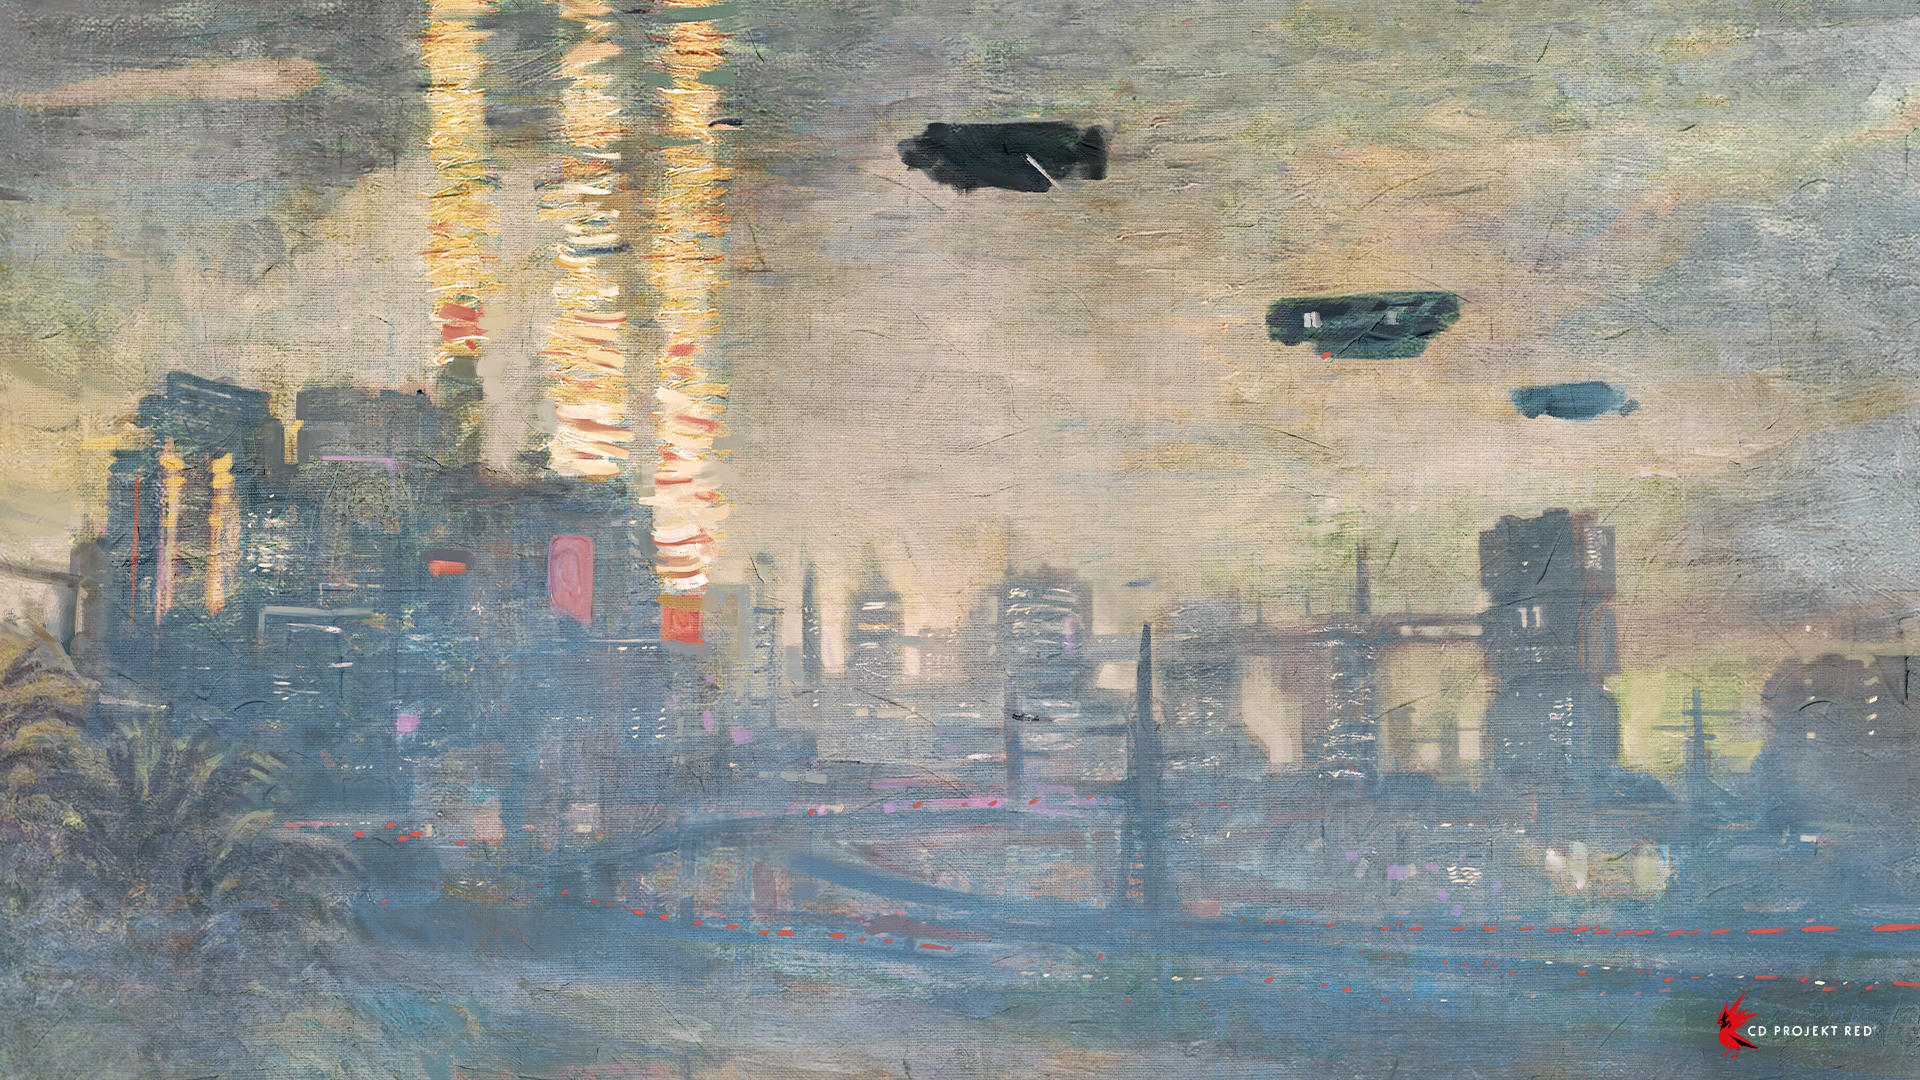
\includegraphics[width=0.88\textwidth]{figures/cover-night-city.jpg}\par

  \vfill

  \begin{minipage}{0.74\textwidth}
    \small\itshape
    The bad news is that we have still a long way to go.\\
    The good news is that we have still a long way to go.

    \medskip
    \normalfont\raggedleft --- Alain Fournier, 1998
  \end{minipage}

  \vspace*{0.07\textheight}
\end{titlepage}


\ytableausetup{centertableaux}






\newpage



\tableofcontents
\newpage


\notesection{2023-12-22}{Tori, Pinnings, and Coherent Continuation}\label{1}

\subsection{Identification of co-character groups with Lie algebras}
Settings: $G$ complex connected reductive algebraic group. $Q \subseteq P \subseteq \fh^*$ are root lattice and weight group, respectively. $\check{Q} \subseteq \check{P} \subseteq \fh$ are coroot lattice and coweight group, respectively. $H$ is a maximal torus of $G$, $\fh$ is its Lie algebra.


There are identifications 
\defmap{I}{X_*(H)\otimes \BC}{\fh}{\phi}{\dd\phi\bra{1}}

\defmap{J}{X^*(H)\otimes \BC}{\fh ^*}{\varphi}{\dd \varphi}



Under these identifications we have

\begin{align*}
  P_* &= \bigset{\check{\lambda} \in \fh}{\bil{\alpha}{\check{\lambda}} \in \BZ, \textrm{for all $\alpha \in Q$}}\\
  & = \bigset{\check{\lambda} \in \fh}{\exp(2\pi\sqrt{-1}\bil{\alpha}{\check{\lambda}}) = 1, \textrm{for all $\alpha \in Q$}}\\
  & = \bigset{\check{\lambda} \in \fh}{\alpha(\exp(2\pi\sqrt{-1}\check{\lambda})) = 1, \textrm{for all $\alpha \in Q$}}\\
  & = \bigset{\check{\lambda} \in \fh}{\exp(2\pi\sqrt{-1}\check{\lambda}) \in Z(G)}.
\end{align*}
And
\begin{align*}
  X_{*}(H) & = \bigset{\check{\lambda} \in \fh}{\bil{\phi}{\check{\lambda}} \in \BZ, \textrm{for all $\phi \in X^*(H)$}}\\
  & = \bigset{\check{\lambda} \in \fh}{\exp(2\pi\sqrt{-1}\bil{\phi}{\check{\lambda}}) = 1, \textrm{for all $\phi \in X^*(H)$}}\\
  & = \bigset{\check{\lambda} \in \fh}{\phi(\exp(2\pi\sqrt{-1}\check{\lambda})) = 1, \textrm{for all $\phi \in X^*(H)$}}\\
  & = \bigset{\check{\lambda} \in \fh}{\exp(2\pi\sqrt{-1}\check{\lambda}) = 1}.
\end{align*} 

Similarly
$$P^* = \bigset{\lambda \in \fh^*}{\exp(2 \pi \sqrt{-1} \lambda) \in Z(\check{G})}. $$

$$X^*(H) = \bigset{\lambda \in \fh^*}{\exp(2 \ pi \sqrt{-1} \lambda ) = 1}.$$


Define $e: \fh \to H$ by $e(X) = \exp(2\pi\sqrt{-1}X)$, then $\ker(e) = X_*(H)$.

\[
\begin{tikzcd}
  \fh \arrow[r,"e"] & H \\
  P_* \arrow[r, "e"] \arrow[u,hook ] & Z(G) \arrow[u,hook]
\end{tikzcd}
\]

$Z(G) \simeq P_*/X_*(H)$.




\subsection{Pinnings of algebraic groups}

\begin{thm}[see \cite{AdC09}]
  Inner automorphism group $\mathrm{Inn(G)}$ of $G$ is equal to $\mathrm{G/Z(G)}$,
  $\mathrm{Inn(G)}$ acts freely and transitively on the set of pinnings.
\end{thm}


I know that there is an analogy in compact connected groups, and it has been proved.

\begin{thm}
  If $\RG$ is a compact connected group, then its inner automorphism group $\mathrm{Inn(G)} = \mathrm{G/Z(G)}$
  acts freely and transitively on the set of pinnings.
  (where pinnings for it is a bit different from the complex case, that $(T, B_\BC,\mathcal{X})$
  is a pinning if $T$ is a maximal torus, $B_\BC$ a Borel of $G_\BC$ containing $T$, $\mathcal{X}$
  is a set of real rays in simple root space.)
\end{thm}

\begin{proof}
  Here's proof from mathoverflow \href{https://mathoverflow.net/questions/377981/classification-of-not-necessarily-connected-compact-lie-groups/378141#378141}{Lspise's answer}:
  \begin{figure}[H]
    \centering
    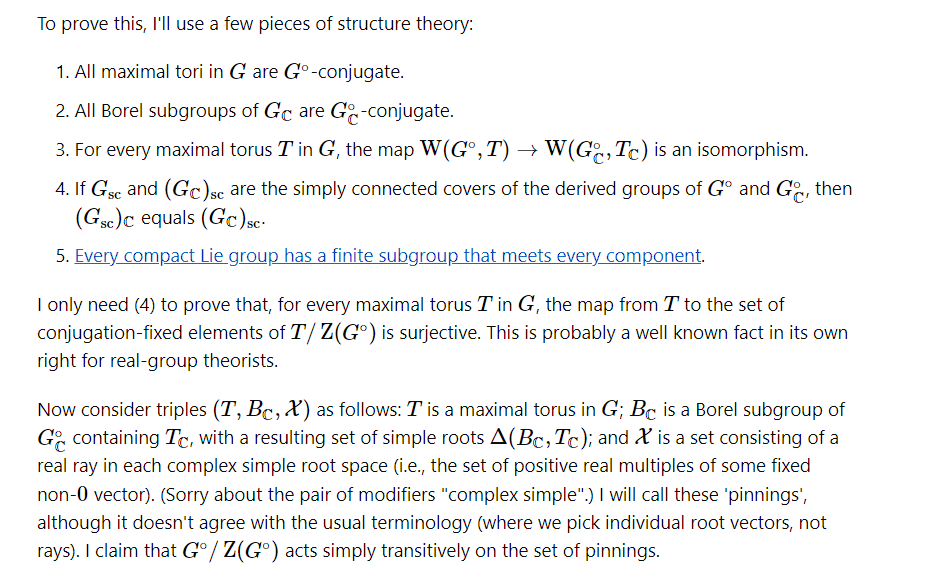
\includegraphics[width=1.0\linewidth]{1.png}
  \end{figure}

  \begin{figure}[H]
    \centering
    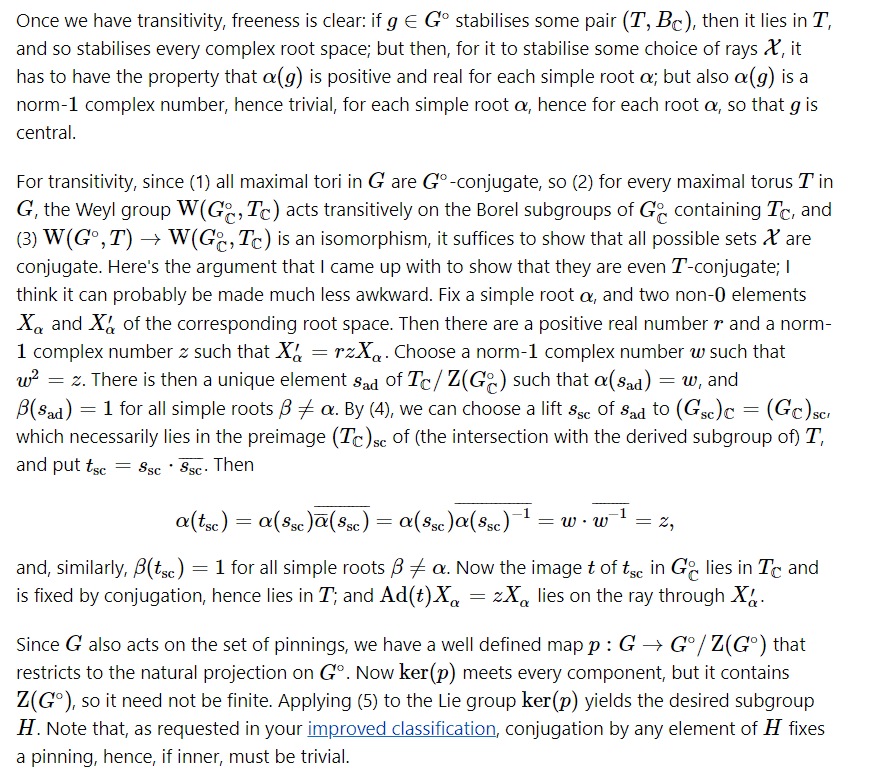
\includegraphics[width=1.0\linewidth]{2.png}
  \end{figure}
\end{proof}



\begin{rk}
  The pinnings show that split reductive algebraic groups look like butterflies!
\end{rk}

\begin{figure}[H]
  \centering
  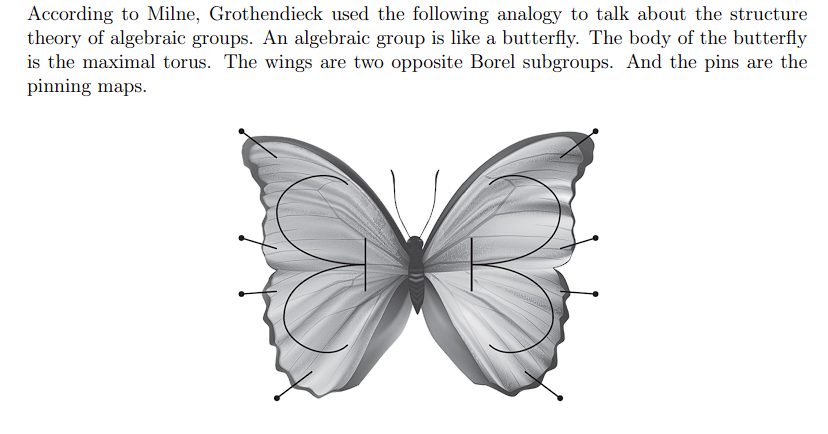
\includegraphics[width=1.0\linewidth]{3.png}
  \caption{Pinning of butterfly}
\end{figure}



\subsection{Coherent continuation representations}

Until the end of today, $G$ denotes a real reductive group in Harish-Chandra class.

Let's recall some basic definitions of coherent continuation representations, in order
for me to do calculations in the case of real classical groups.


Fix a connected reductive complex Lie group $G_\BC$, together with a Lie group homomorphism
$\iota: G \to  G_\BC$ such that its differential $\mathrm{d\iota} : \mathrm{Lie(G)} \to \mathrm{Lie(G_\BC)}$
has the following two properties:
\begin{enumerate}
  \item the kernel of $\mathrm{d\iota}$ is contained in the center of $\mathrm{Lie(G)}$;
  \item the image of $\mathrm{d\iota}$ is a real form of $\mathrm{Lie(G)}$.
\end{enumerate}

The analytical weight lattice of $\mathrm{G_\BC}$ is identified with a subgroup of $^{a}\fh^*$ via $\mathrm{d\iota}$.
We write $Q_\iota \subset \  ^{a}\fh^*$ for this subgroup. Denote root lattice by $Q_\fg$,
weight lattice by $Q^\fg$, then $$Q_\fg \subset Q_\iota \subset Q^\fg.$$
They are all $W$ stable subgroups.
And we have some categories:
\begin{enumerate}
  \item $\mathrm{Rep}(\fg,Q_\iota)$ the category of all finite-dimensional representations of $\fg$ whose weight are contained in $Q_\fg$, \textcolor{AttentionColor}{it can be identified with $\mathrm{Rep(Lie(G_\BC),Q_\iota)}$ and hence $\mathrm{Rep_{finite}(G_\BC)}$};
  \item $\mathrm{Rep(G)}$ the category of all Casselman-Wallach representations of $G$, and its full subcategories $\mathrm{Rep_\mu(G)}$, $\mathrm{Rep_S(G)}$.
\end{enumerate}
To denote their Grothendieck groups, we replace $\mathrm{Rep}$ by $\mathcal{K}$.


Fix a $Q_\iota$-coset $\Lambda = \lambda + Q_\iota \subset \  ^{a}\fh^*$.


\begin{defn}[coherent family]
  A $\mathcal{K}(G)$-valued $\Lambda$ coherent family is a map
  $$\varPhi : \Lambda \to \mathcal{K}(G)$$
  satisfies the following two conditions:
  \begin{enumerate}
    \item for all $\nu \in \Lambda$, $\varPhi(\nu) \in \mathcal{K}_{\nu}(G)$;
    \item for all representations $F \mathrm{ \in Rep}(\fg,Q_\iota)$ and all $\nu \in \Lambda$,
          $$F \cdot (\varPhi(\nu)) = \sum\limits_{\mu} \varPhi(\nu + \mu),$$
          where $\mu$ runs over all weights of $\mathrm{F}$, counted with multiplicities.
  \end{enumerate}
  The set of coherent families is denoted by $\mathrm{Coh}_\Lambda(\mathcal{K}(G))$
\end{defn}
We have the integral Weyl group $W_{\Lambda} = \set{w \in W}{w\lambda - \lambda \in Q_\iota}$
there is a representation of $W_\Lambda$ on $\mathrm{Coh}_\Lambda(\mathcal{K}(G))$ by
$$(w \cdot \varPhi)(\nu) = \varPhi (w^{-1}\nu).$$
This is called a coherent continuation representation.




\notesection{2023-12-23}{Regular Parameters and Outer Automorphisms}\label{2}

\subsection{Review of regular parameter}

Following yesterday's discussion of coherent continuation representations, we define two basis
for it, use Langland classification, follow \cite{BMSZ22}.

Suppose $H$ is a Cartan subgroup of $G$, by which we mean a subgroup that is the centralizer of
a Cartan subalgebra of $\Lie(G)$ \textcolor{ClarificationColor}{(In the case of linear groups, it's just a
  real algebraic torus.)}. $H$ has a unique maximal compact subgroup (since $G$ is in Harish-Chandra's
class, adjoint representation of $H$ is trivial, $H_0$ lies in the center of $H$, as we know, all
maximal subgroups of Lie groups are conjugate to each other, use Cartan decomposition of $H$, we win. In fact,
$H$ has a unique maximal compact torus and a unique maximal split torus)
We denote by $\Delta_{\fh} \subset \fh^*$ the root system of $\fg$. A root is called imaginary
if $\check{\alpha } \in \ft$ (i.e. roots which take pure imaginary values on $\Lie(H)$), an imaginary root $\alpha$ is
called compact if $\fg_{\alpha}$ and $\fg_{-\alpha}$ is contained in the complexified Lie algebra of a common compact subgroup of $G$.(this is equivalent to $\fg_\alpha $ belong to a Lie subalgebra of a compact subgroup, since $\fg_\alpha $ lies in a Lie subalgebra of maximal compact subgroup is equivalent to $\fg_{-\alpha }$ Lies in the same subgroup)


There are two important facts about the representation theory of $H$:
\begin{enumerate}
  \item Every Casselman-Wallach representation of $H$ is finite-dimensional, it follows directly from that $H$ is an extension of an abelian group and a finite group;
  \item For every $\Gamma \in \mathrm{Irr(H)}$ differential of $\Gamma$ is a direct sum of one-dimensional representations attached to a unique $\mathrm{d\Gamma \in \fh^*}$.
        (it is true because $H$ is in Harish-Chandra's class).
\end{enumerate}


For every Borel subalgebra $\fb$ of $\fg$ containing $\fh$, write 
$$\xi_{\fb}: \fh \to \ ^{a}\fh,$$
for the linear isomorphism attached to $\fb$ defined by 
$$\fh \hookrightarrow  \fb \to \fb / \sqbra{\fb,\fb} = \ {^{a}\fh}.$$
The transpose inverse of this map is still denoted by $\xi_{\fb}: \ ^{a}\fh^* \to \fh^*$.\\


Write $$W\bra{^{a}\fh^*,\fh^*} :=  \set{\xi_{\fb}: \ ^{a}\fh^* \to \fh^*}{\fb \ \textrm{is a Borel subalgebra containing} \ \fh}.$$

\begin{defn}
  For every element $\xi \in W\bra{^{a}\fh^*,\fh^*}$, put
  $$\delta(\xi) := \frac{1}{2} \cdot \sum\limits_{\alpha  \ \textrm{is an imaginary root in} \ \xi\Delta^+}\alpha - \sum\limits_{\beta \ \textrm{is an compact imaginary root in} \ \xi\Delta^+}\beta \in \fh^* .$$
  Write $\mathcal{P} _{\Lambda}(G)$ for the set of all triples $\gamma = (H,\xi,\Gamma)$, where
  $H$ is a Cartan subgroup of $G$, $\xi \in W\bra{^{a}\fh^*,\fh^*}$, and
  \defmap{\Gamma}{\Lambda}{\Irr(H)}{\nu}{\Gamma_{\nu}}
  is a map with the following properties:
  \begin{enumerate}
    \item $\Gamma_{\nu+\beta} = \Gamma_{\nu} \otimes \xi(\beta)$ for all $\beta \in Q_{\iota}$ and $\nu \in \Lambda$;
    \item $\mathrm{d\Gamma_{\nu}} = \xi(\nu) + \delta(\xi)$ for all $\nu \in \Lambda$.\textcolor{NoteColor}{(note that Cartan subgroups not always have irr repn with this differential!)}
  \end{enumerate}
  Here $\xi(\beta)$ is naturally viewed as a character of $H$ by using the homomorphism
  $\iota : H \to H_{\BC}$, and $H_{\BC}$ is a Cartan subgroup of $G_{\BC}$ containing $\iota(H)$.
\end{defn}



\subsection{Outer automorphism of algebraic groups}

\begin{lem}[a simple discover of abstract algebra]
  $G$ an abstract group, $H$ a normal subgroup of $G$, if $G$ acts
  transitively on a set $X$ such that the restriction of this action
  to $H$ is free and transitive, then the short exact sequence of groups
  $$\shortexact{1}{H}{G}{G/H}{1}$$
\end{lem}

\begin{proof}
  Actually choose an element $x \in X$, we have
  $$ G \simeq \mathrm{Stab}_{G}(x) \ltimes H.$$
\end{proof}


Using this lemma, we can see that for a complex connected reductive
algebraic group $G$, $\Aut(G)$ acts on the set of pinnings transitively,
with its normal subgroup the $\Inn(G)$ acts freely and transitively,
so every pinning gives us a split of the short exact sequence
$$\shortexact{1}{\Inn(G)}{\Aut(G)}{\Out(G)}{1}.$$


Some facts about split connected reductive algebraic groups over arbitrary field $k$:
\begin{enumerate}
  \item $\{ \textrm{split connected reductive algebraic groups} \}/_\backsim \ = \{ \textrm{root datums}\} /_\backsim $;
  \item For any two automorphisms of $G$, if they induce the same automorphism of root datum, then they differ by an inner automorphism;
  \item Fix a pinning, we get an isomorphism $\Out(G) \simeq \Aut(D_b)$.
\end{enumerate}



\section{2024.2.27 Young diagrams}\label{4}
Some code examples of Young diagrams and tableaux using the \texttt{ytableau} package:

\begin{ytableau}
  \none[2] &  &  & \none \\
  \none[1]  &  &  &  \\
  \none & \none[1] & \none[2] & \none[3]
\end{ytableau}

\ydiagram{1,2,1}



\[
  \begin{ytableau}
    \none &  & \cdots &\\
    ~ & \none & \none & \none \\
    ~ & \none & \none & \none \\
    \vdots & \none & \none & \none \\
    x & \none & \none & \none
  \end{ytableau}
  ~+~
  \begin{ytableau}
    ~ & \none & \none & \none & \none\\
    ~ & \none & \none & \none & \none\\
    \vdots & \none & \none & \none & \none\\
    x &  &  & \cdots &
  \end{ytableau}
  ~=~
  \begin{ytableau}
    ~ & \none & \none & \none & \none\\
    ~ & \none & \none & \none & \none\\
    \vdots & \none & \none & \none & \none\\
    x & \none & \none & \none & \none\\
    ~ &  &  & \cdots &
  \end{ytableau}
\]


% 综合示例
\[
\begin{ytableau}
*(blue) a & *(yellow) b & *(green) c \\ 
*(red) 1 & 2 \\
3
\end{ytableau}
\]

% 水平对齐
\[
\begin{ytableau}
~ & ~ & ~ \\ 
~ & ~ \\
~
\end{ytableau}
\hspace{3em}
\begin{ytableau}
~ & ~ \\
~ & ~ \\
~ 
\end{ytableau}
\]

% 垂直对齐
\[
\begin{array}{c}
\begin{ytableau}
~ & ~ & ~ \\ 
~ & ~ \\
~
\end{ytableau} \\[3em]
\begin{ytableau}
~ & ~ \\
~ & ~ \\
~ 
\end{ytableau}
\end{array}
\]

% 基线对齐
ce est chinois
$\vcenter{\hbox{\begin{ytableau}
~ & ~ \\ 
~
\end{ytableau}}}$
english

\[
a = \vcenter{\hbox{\begin{ytableau}
~ & ~ \\ 
~
\end{ytableau}}} + b
\]

% 综合示例
\[
\begin{array}{cc}
\text{youngdiagram1: } & \vcenter{\hbox{\begin{ytableau}
~ & ~ & ~ \\ 
~ & ~ \\
~
\end{ytableau}}} \\[3em]
\text{young2: } & \vcenter{\hbox{\begin{ytableau}
~ & ~ \\
~
\end{ytableau}}}
\end{array}
\]

For a compact connected Lie group $G$, choose a maximal torus $T$, there is a canonical 1-1 correspondence:

$$X^*(T)/W \longleftrightarrow (X^*(T)+\rho)/W \longleftrightarrow \mathrm{Irr}(G)$$

Moreover, if we choose a positive system $\Psi^+$, and then $\rho_{\Psi^+}$, the above sets also canonically isomorphic to the set of dominant analytically integral weights:
$$\set{\lambda \in X^*(T)}{ \langle\lambda, \alpha \rangle \geq 0, \text{for all} \ \alpha \in \Psi^+ }$$

This can be generalized to parameter of discrete series representations for connected semisimple Lie groups $G$ with compact Cartan subgroup $T$ :

$$ (X^*(T) + \rho)^{reg}/W_c$$

If a discrete series representation $V$ has minimal $K$ type which has maximal weight $\nu$, then it's parameter is $\lambda = \nu -\rho + 2\rho_c $.\textcolor{AttentionColor}{(not sure)}

Note that for a fixed infinitesimal character, there are exactly $|W/W_c|$ different discrete series representations.



\section{2024.2.28 Continuous complex characters}\label{5}
Some facts about continuous complex characters of some common abelian topological groups:

\begin{tabular}{|c|c|c|}
  \hline
  field            & character group & correspondence                                \\
  \hline
  $(\BR^\times_+,\times)$        & $\BC$           & $\xi \mapsto (t \mapsto t^\xi)$ \\
  \hline
  $(\BC^\times,\times) $ &    $\BC \times \BZ$             & $(\xi,n) \mapsto (z \mapsto |z|^\xi (\frac{z}{|z|})^n)$                                              \\
  \hline
  $(\BS^1,\times)$          &  $\BZ$               & $n \mapsto (z \mapsto z^n)$                                              \\
  \hline
  $(\BQ_p,+)$          & $\BQ_p$                 &  $\xi \mapsto (x \mapsto \mathrm{exp}(2\pi i \xi \{ x \}_p))$                                             \\
  \hline
\end{tabular}

\begin{rk}
  Note that all continuous characters of $\BQ_p$ are automatically locally constant (smooth), which is consistent with the case of real lie groups. 
\end{rk}



\section{2024.10.22 Associated variety of irreducible Casselman-Wallach representations}

\begin{lem}
  The associated variety of an irreducible Casselman-Wallach representation of a real reductive group in Harish-Chandra class is the closure of a nilpotent orbit in $\fg^*$.
\end{lem}

\begin{proof}
  By the work of Borho, Brylinski \cite{BB82}, and Joseph \cite{Jos85}, the associated variety of any primitive ideal (annihilator of an irreducible $\fg$-module) is the closure of a single nilpotent orbit. So we only need to prove that $\mathrm{gr}(\mathrm{Ann_{\CU(\fg)}(V)})$ is a primitive ideal.

  Since the $K$-finite part $V_K$ is dense in $V$, $\Ann_{\CU(\fg)}(V) = \Ann_{\CU(\fg)}(V_K)$, we only need to consider the annihilator of the irreducible $(\fg,K)$-module $V_K$.

  If $G$ is connected, then $K$ is also connected, so $V_K$ is irreducible as $\CU(\fg)$-module, in this case, $\Ann_{\CU(\fg)}(V)$ is a primitive ideal.

  If $G$ is not connected, let $G_0$ be the identity component of $G$, $K_0 = G_0 \cap K$ is a maximal compact subgroup of $G_0$, then $V_K|_{G_0}$ is a finite length $(\fg,K_0)$-module, it has an irreducible quotient $V_K \to V_0$, then according to the theory of induction of $(\fg,K)$-modules \cite[Chapter 2]{KV95} we have an injective morphism of $(\fg,K_0)$-modules:
  \begin{equation}
     V_K|_{K_0} \hookrightarrow  (\mathrm{induced}_{K_0}^{K}(V_0))|_{K_0} \cong \bigoplus_{\textrm{double cosets} \ K_0 k K_0} kV_0,
  \end{equation}
  where $kV_0$ be the $(\fg,K_0)$-module whose underlying space is $V_0$, whose action by $X \in \fg$ is the usual action by $\Ad(k)X$, whose action by $g \in K_0$ is the usual action by $k^{-1}gk$, it has the same annihilator in $\CU(\fg)$ as $V_0$ since $G$ is in Harish-Chandra's class, and hence the annihilator of $V_K$ is the same as the annihilator of $V_0$, which is a primitive ideal.

\end{proof}



\section{2024.11.28 Split reductive algebraic groups over arbitrary field}
Any split connected reductive group over arbitrary field can be uniquely defined and split over $\BZ$. (Chevalley group)

Classification of split reductive group is the same over arbitrary non-empty schemes, which is equivalent to the classification of root data.(cf. \cite{SGA3})




\section{2024.12.17 Geometric Pre-quantization}

\textbf{Geometric Pre-quantization}

Let $X$ be a smooth manifold. There are natural maps
\[
    \mathrm{Pic}(X) \longrightarrow  \mathrm{H}^{2}_{\text{dR}}(X;\BR) \simeq  \mathrm{H}^{2}_{\text{\v{C}ech}}(X;\BR).
\]
Construction of the first map:
For a (complex) line bundle $\BL \in \mathrm{Pic}^{h}(X)$, let $\langle , \rangle$ be a Hermitian metric on it and $\nabla$ be a unitary connection. (Every line bundle $\BL \in \mathrm{Pic}(X)$ has a Hermitian metric and a unitary connection on it.) 
\begin{itemize}
  \item choose a locally trivialization $\{U_{\alpha}\}$ of $\BL$, such that all $U_{\alpha}$ and $U_{\alpha} \cap U_{\beta}$ are contractible;
  \item choose Unitary local frames $\{s_{\alpha}\}$ for $\BL$ on each $U_{\alpha}$, then $s \leftrightarrow (f_\alpha)$ and $\nabla \leftrightarrow (\theta_\alpha)$ (unitary implies that $\theta_\alpha$ are pure imaginary);
  \item define $\Omega := \mathrm{d}\theta_\alpha$, and $c_1(\BL) := [\frac{1}{2\pi i}\Omega] \in \mathrm{H}^{2}_{dR}(X;\BR)$ ($\Omega = \mathrm{curv}\nabla$).
\end{itemize}
$c_1(\BL)$ is independent of the choice of $\langle,\rangle$ and $\nabla$ by Chern-Weil theory.
And we can see that $\theta_\alpha - \theta_\beta = \frac{\mathrm{d}g_{\alpha,\beta}}{g_{\alpha,\beta}} = \mathrm{d}\mathrm{log}(g_{\alpha,\beta})$ on $U_\alpha \cap U_\beta$, where $g_{\alpha,\beta}$ is the translation function ($s_\beta = g_{\alpha,\beta}s_\alpha$).

Construction of the second map (classical de-Rham isomorphism), choose a 2-form $\omega \in \mathrm{H}^{2}_{dR}(X;\BR)$
\begin{itemize}
  \item choose a cover $\{U_{\alpha}\}$ of $\BL$, such that all $U_{\alpha}$ and $U_{\alpha} \cap U_{\beta}$ are contractible;
  \item on each $U_\alpha$, choose a 1-form $\theta_\alpha$ such that $\mathrm{d}\theta_\alpha = \omega|_{U_\alpha}$;
  \item since $\mathrm{d}\theta_\alpha = \mathrm{d}\theta_\beta$ on $U_\alpha \cap U_\beta$, we can choose smooth function $c_{\alpha,\beta}$ such that $\mathrm{d}c_{\alpha,\beta} = \theta_\alpha - \theta_\beta$;
  \item let $c_{\alpha,\beta,\gamma} = c_{\alpha,\beta} + c_{\beta,\gamma} + c_{\gamma,\alpha}$, which is a constant, and we get the corresponding 2-cocycle $(c_{\alpha,\beta,\gamma}) \in \mathrm{H}^{2}_{\text{\v{C}ech}}(X;\BR)$.
\end{itemize}

If $\omega$ come from the first map, we can choose $c_{\alpha,\beta} = \frac{1}{2\pi i}\mathrm{log}g_{\alpha,\beta}$, and hence $c_{\alpha,\beta,\gamma} = \frac{1}{2\pi i}(\mathrm{log}g_{\alpha,\beta} +\mathrm{log}g_{\beta,\gamma} +\mathrm{log}g_{\gamma,\alpha} ) \in \BZ$. So the morphism is in fact

\[
    \mathrm{Pic}(X) \longrightarrow  \mathrm{H}^{2}_{dR}(X;\BZ) \simeq  \mathrm{H}^{2}_{\text{\v{C}ech}}(X;\BZ).
\]

In fact the first map is also an isomorphism. (cf. \href{http://staff.ustc.edu.cn/~wangzuoq/Courses/15S-Symp/SympGeom.html}{prequantization})
For a 2-form $\omega$, choose $\theta_\alpha$ and $c_{\alpha,\beta}$ as above, let $g_{\alpha,\beta} = \exp(2\pi i c_{\alpha,\beta})$, these are transition functions of a complex line bundle $\BL$.

\begin{cor}
  Assume that $G$ is a connected Lie group. The following are equivalent:
  \begin{itemize}
    \item $\Omega \subseteq \fg^*$ is integral ($[\sigma_{\Omega}] \in \mathrm{H}^2(X;\BZ)$);
    \item there exists a $G$-equivariant complex line bundle over $\Omega$ with a $G$-invariant Hermitian connection $\nabla$ such that $$\frac{1}{2\pi i}\mathrm{curv}\bra{\nabla} = \sigma_{\Omega}.$$
  \end{itemize}
\end{cor}

\begin{figure}[H]
  \centering
  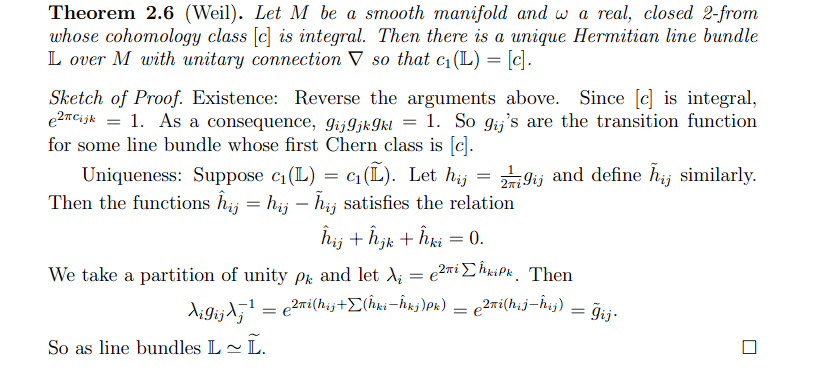
\includegraphics[width=1.0\linewidth]{4.png}
  \caption{Proof}
\end{figure}



\notesection{2025-08-14}{\texorpdfstring{Tianyuan Problems \protect\footnote{This section is organized by Ryan Ang and Qiutong Wang at Tianyuan Mathematics Research Centre.}}{Tianyuan Problems}}


Let $G$ be a finite central extension of an open subgroup of $\mathbb{R}$-points of a connected reductive algebraic group (reductive Nash group \cite{Sun15}) with Lie algebra $\mathfrak{g}$. Fix an invariant nondegenerate bilinear form $B(-,-)$ on $\mathfrak{g}$.


For an irreducible Casselman-Wallach representation $\pi$ of $G$, let $\mathrm{Wh}_\mathcal{O}(\pi)$ be the space of generalized Whittaker models of $\pi$ associated to the nilpotent orbit $\mathcal{O}$. Let
\[\mathrm{WO}(\pi):= \set{\mathcal{O}}{\textrm{$\mathcal{O}$ is a nilpotent orbit such that $\mathrm{Wh_{\mathcal{O}}(\pi) \neq 0}$}},\]
and the \textit{Whittaker support} $\mathrm{WS}(\pi)$ of $\pi$ be the set of all maximal orbits in $\mathrm{WO}(\pi)$ with respect to closure inclusion:
\[\mathrm{WS}(\pi) := \set{\mathcal{O}}{\textrm{$\mathcal{O}$ is a maximal orbit in $\mathrm{WO}(\pi)$} }.\]




Another nilpotent invariant is the wavefront cycle:
\[\mathcal{WF}(\pi) = \sum_{i}m_i [\mathcal{O}_i].\]
With the corresponding wavefront set :
\[\mathrm{WF}(\pi) = \bigcup\limits_{m_i \neq 0} \overline{\mathcal{O}_i}. \]



M{\oe}glin-Waldspurger \cite{MW87} proved that $\mathrm{WF}(\pi)=\mathrm{WS}(\pi)$ when $F$ is a $p$-adic field. We want to test this conjecture for arbitrary reductive almost linear Nash groups.
\begin{conj}[Main conjecture] For any reductive almost linear Nash group $G$ and any irreducible Casselman-Wallach representation $\pi$:
      \[\mathrm{WF}(\pi)=\mathrm{WS}(\pi).\]
\end{conj}

Take a nilpotent orbit $\mathcal{O} \subseteq \mathfrak{g}$ (or $\mathfrak{sl_2}$-triple $\gamma = \{Y,H,X\}$ in $\mathfrak{g}$). $\mathfrak{g}/\mathfrak{g}^{Y}$ is a symplectic space with symplectic form $\left \langle -,- \right \rangle := B(Y,[-,-])$. Set $G^{Y} := \Stab_{G}(Y)$, there is a natural homomorphism $G^{Y} \to \Sp(\mathfrak{g}/\mathfrak{g}^{Y},\left\langle -,- \right\rangle)$. Let $\widetilde{G^{Y}}$ be the double cover of $G^{Y}$ induced by the metaplectic double cover of $\Sp(\mathfrak{g}/\mathfrak{g}^{Y},\left\langle -,- \right\rangle)$.
\begin{defn}
   The nilpotent $\mathcal{O}$ is called admissible if the double cover $\widetilde{G^Y}$ is split over the identity component of $(G^Y)_0$. It is called quasi-admissible if $\widetilde{G^Y}$ has a finite-dimensional genuine representation.
\end{defn}

Result of \cite{GGS21} says that $\mathrm{WS}(\pi)$ consists of quasi-admissible orbits. But they do not know whether the non-admissible quasi-admissible orbits appear in Whittaker supports of representations. We may ask the same question for the wavefront set:

\textbf{Problem 1}: Are all the nilpotent orbits in the wavefront cycle admissible?

\medskip

For the case when $G$ is general linear, it is well known that the wavefront set $\mathrm{WF}(\pi)$ of an irreducible Casselman-Wallach representation $\pi$ of $G$ consists of a single nilpotent adjoint orbit. Together with some counting results, it maybe possible to construct all irreducible representations of general linear group via theta correspondence and coherent continuation.

\textbf{Problem 2}: Can we construct all irreducible representations via theta correspondence, coherent continuation, and twist of characters?

Assuming the construction steps above are done, it then remains to study the Whittaker support $\mathrm{WS}(\pi)$ of $\pi$. We focus on two types of interactions with Whittaker models - theta correspondence and coherent continuation.



On one hand, Gomez-Zhu \cite{GZ14} proved for type I reductive (symplectic-orthogonal) dual pairs in the stable range that the big theta lift preserves the structure of Whittaker models:
\[\mathrm{Wh}_{\Theta(\mathcal{O})}\left(\Theta(\pi)\right)=\mathrm{Wh}_\mathcal{O}(\pi^\vee).\]
Noting that $(G,G')=(\GL_n(F),\GL_m(F))$ is a (reductive) dual pair for any $n,m\in\mathbb{N}$, one observes that if one can prove an analogue of Gomez-Zhu's result for type II dual pairs, one can use it to infer properties of the structure of the Whittaker support $\mathrm{WS}(\pi)$. Hence we propose the following subconjecture:
\begin{conj}
    If $(G,G')=(\GL_n(F),\GL_m(F))$ is a type II reductive dual pair over $F$ in the stable range (with $n\leq m$), and $\pi$ is a genuine Casselman-Wallach representation of $G$, then
    \[\mathrm{Wh}_{\Theta(\mathcal{O})}\left(\Theta(\pi)\right)=\mathrm{Wh}_\mathcal{O}(\pi^\vee),\]
    where $\pi^\vee$ denotes the smooth contragredient of $\pi$. Furthermore, the above will imply that
    \[\mathrm{WS}\left(\Theta(\pi)\right)=\mathrm{WS}(\pi^\vee).\]
\end{conj}

On the other hand, Barbash-Vogan \cite{BV80} proved that under coherent continuation, the multiplicity of wavefront cycle changes in the form of a Goldie rank polynomial, i.e.
\[
    \mathcal{WF}(\pi(\lambda)) = p(\lambda) \cdot (\sum\limits_{i} c_i [\mathcal{O}_i]),
\]
where $p(\lambda)$ is the goldie rank polynomial, $\lambda$ is dominant. We expect some similar result for the multiplicity of the generalized Whittaker model.

\textbf{Problem 3}: For a fixed nilpotent orbit $\mathcal{O}$, does there exist a constant $c_{\mathcal{O}}$ such that $\dim \mathrm{Wh}_{\mathcal{O}}(\pi(\lambda)) = c_{\mathcal{O}} \cdot p(\lambda)$?





\notesection{2025-10-01}{Orbit Method and Wavefront Sets}

Orbit method for nilpotent Lie groups.

Let $G$ be a connected, simply connected nilpotent Lie group with Lie algebra $\fg$. Let $\fg^*$ be the dual space of $\fg$.

We have Fourier transform:
\[
    \mathcal{F} : \mathcal{S}(\fg)\dd X \to \mathcal{S}(\sqrt{-1}\fg^*), \quad f\dd X \mapsto \widehat{f\dd X}, \quad \widehat{f\dd X}(l) = \int_{\fg} f(X) e^{\langle l,X\rangle} \dd X.
\]

Take its dual:
\[
    \mathcal{S}'(\sqrt{-1}\fg^*) \to (\mathcal{S}(\fg)\dd X)', \quad T \mapsto \check{T}, \quad \langle \check{T}, f\dd X \rangle = \langle T, \widehat{f\dd X} \rangle.
\]

For any irreducible unitary representation $\pi$ of $G$, we have its character $\Theta_\pi \in C^{-\infty}(G)$ defined by
\[\Theta_\pi(f) = \Tr\bra{\pi\bra{f\mathrm{dg}}}, \quad f\mathrm{dg} \in C_c^\infty(G)\mathrm{dg}.\]
Using the exponential map $\exp : \fg \to G$ (isomorphism in this case), we can view $\Theta_\pi$ as a distribution on $\fg$:
\[\theta_\pi(f\mathrm{dX}) = \Theta_\pi(f \circ \exp), \quad f\mathrm{dX} \in C_{c}^{\infty}(\fg)\mathrm{dX}.\]
In fact, $\theta_{\pi}$ is a tempered generalized function on $\fg$ (it can continuously extends to $\mathcal{S}(\fg)\mathrm{dX}$).
By the work of Howe, Kirillov, and others, we have the following theorem:
\begin{thm}
    There exists a unique coadjoint orbit $\mathcal{O} \subseteq \sqrt{-1}\fg^*$ such that $\check{\theta}_\pi = \mu_{\mathcal{O}}$, where $\mu_{\mathcal{O}}$ is the canonical measure on $\mathcal{O}$.
\end{thm}

This defines a bijection between $\widehat{G}$ (the unitary dual of $G$) and the set of coadjoint orbits in $\sqrt{-1}\fg^*$.

Conversely, for any coadjoint orbit $\mathcal{O} \subseteq \sqrt{-1}\fg^*$, we can construct an irreducible unitary representation $\pi_{\mathcal{O}}$ of $G$ such that $\check{\theta}_{\pi_{\mathcal{O}}} = \mu_{\mathcal{O}}$. This is the more interesting part, use the method of geometric quantization.

Take any element $\lambda \in \mathcal{O}$, we have an identification $\mathcal{O} = G/G_{\lambda}$, $lambda: \fg_{\lambda} \to \BC$ is a Lie algebra homomorphism, and hence $\chi_{\lambda} : G_{\lambda} \to \BC^\times$ defined by $\chi_{\lambda}(\exp X) = e^{\langle \lambda,X \rangle}$ is a unitary character of $G_{\lambda}$. Then we can defined a Hermitian line bundle $\mathcal{L}_{\lambda} = G \times^{G_{\lambda}} \BC$ over $\mathcal{O}$, with a natural $G$-invariant connection $\nabla$ such that $\mathrm{curv}(\nabla) = \omega_{\mathcal{O}}$, where $\omega_{\mathcal{O}}$ is the Kirillov-Kostant-Souriau symplectic form on $\mathcal{O}$.

Then we can define the Hilbert space of square integrable sections of $\mathcal{L}_{\lambda}$, but this space is too large. We need to choose a polarization $\mathfrak{h} \subseteq \fg_{\BC}$ (maximal isotropic subalgebra with respect to the bilinear form $(X,Y) \mapsto \langle \lambda, [X,Y] \rangle$) and consider the space of square integrable holomorphic sections of $\mathcal{L}_{\lambda}$ which are covariant constant along $\mathfrak{h}$.

In fact the polarization $\mathfrak{h}$ corresponds to a $G$-invariant integrable distribution on $\mathcal{O}$, its a subbundle $P$ of $T\mathcal{O}$ each fiber is a lagrangian subspace.
Then we can define the space of polarized sections:
\[\Gamma_P(\mathcal{O},\mathcal{L}_{\lambda}) = \set{s \in \Gamma^{\infty}(\mathcal{O},\mathcal{L}_{\lambda} \otimes \abs{\omega_{\mathcal{O/P}}}^{\frac{1}{2}})}{\nabla_X s = 0, \forall X \in P}.\]

On this space, we have a unitary $G$ action and get a unitary representation $\pi_{\mathcal{O}}$ of $G$, it turns out that $\pi_{\mathcal{O}}$ is irreducible and independent of the choice of the polarization $\mathfrak{h}$.

Kirillov's philosophy works well for nilpotent Lie groups, but for more general Lie groups, it is not true anymore.


Now assume $G$ is a real reductive group, with Lie algebra $\fg_0$. For any irreducible Casselman-Wallach representation $\pi$ of $G$, we still have its generalized function character $\Theta_\pi \in C^{-\infty}(G)$, and hence a tempered generalized function $\theta_\pi$ on $\fg$. Here $\theta_{\pi} \in C^{-\infty}(\fg_0)$ is defined as follows:
\[\theta_\pi(f\mathrm{dX}) = \Theta_\pi(\exp_{*}(\sqrt{\mathrm{det(exp)}}f\mathrm{dX})), \quad f\mathrm{dX} \in C_{c}^{\infty}(\fg_0)\mathrm{dX}.\]

The generalized function $\Theta_{\pi}$ has the following properties:
\begin{itemize}
    \item $\Theta_{\pi}$ is invariant under conjugation of $G$;
    \item $\Theta_{\pi}$ is an eigendistribution of $\CU(\fg)^{G}$;
    \item $\Theta_{\pi}$ is locally integrable, and real analytic on the regular semisimple locus $G^{\mathrm{rs}}$.
\end{itemize}

By the work of Rossmann, we have the following theorem:
\begin{thm}
    If $\pi$ is tempered, then
    \[
        \theta_{\pi}|_{\textrm{nbhd of 0}} = \sum_{i} c_i \widehat{\mu_{\mathcal{O}_i}}|_{\textrm{nbhd of 0}}.
    \]
    Here $\mu_{\CO_i} \in \mathcal{S}(\sqrt{-1}\fg_0^*)$, is the orbital integral along $\CO_i$.
\end{thm}

For an arbitrary generalized function $\Theta \in C^{-\infty}(M)$, we can define its wavefront set $\mathrm{WF}(\Theta) \subseteq \sqrt{-1}T^*M$ as follows:
\begin{defn}
    For any $(x,\xi) \in \sqrt{-1}T^*M$, $(x,\xi) \notin \mathrm{WF}(\Theta)$ if there exists a compactly supported smooth function $\varphi$ on $M$ such that $\varphi(x) \neq 0$, and an open conic neighborhood $\Gamma$ of $\xi$ such that for any $N \in \BN$, there exists a constant $C_N > 0$ such that
    \[\abs{\widehat{\varphi \Theta}(t\eta)} \leq C_N t^{-N}, \quad \forall t > 0, \eta \in \Gamma.\]
\end{defn}
$\mathrm{WF}(\Theta)$ is a closed conic subset of $\sqrt{-1}T^*M$ (singular direction of $\Theta$).

In particular, we can define the wavefront set $\mathrm{WF}(\pi)$ of an irreducible Casselman-Wallach representation $\pi$ of $G$ as $\mathrm{WF}(\Theta_{\pi}) \cap (\sqrt{-1}T^*_1(G))$, it is a closed conic $G$-invariant subset of $\sqrt{-1}\fg_0^*$. The GK-dimension of $\pi$ is defined as
\[\mathrm{Dim}(\pi) = \frac{1}{2}\dim(\mathrm{WF}(\pi)).\]

$\theta_{\pi}$ is a real analytical function on $\fg_0^{\mathrm{rs}}$, and
\[ \theta^{*}_{\pi}(X) :=  \lim_{t \to 0}t^{\mathrm{Dim}(\pi)}\theta_{\pi}(tX)\]
is still a real analytical function on $\fg_0^{\mathrm{rs}}$, where $\mathcal{B}$ is the flag variety of $G$. We can consider it as in $C^{-\infty}(\fg_0)$.

\begin{thm}(Barbasch-Vogan)
     The asymptotic of $\theta_{\pi}$ defined above is a non-negative linear combination of Fourier transforms of nilpotent orbital integrals:
      \[
          \theta^*_{\pi} = \sum_{i} c_i \widehat{\mu_{\mathcal{O}_i}}.
      \]
      Here $\mu_{\CO_i} \in \mathcal{S}(\sqrt{-1}\fg_0^*)$, is the orbital integral along $\CO_i$.
\end{thm}

$\mathrm{WF}(\pi) = \bigcup_{c_i \neq 0} \overline{\CO_i}$.



\notesection{2025-10-02}{Conormal Bundles and Characteristic Cycles}


\subsection{Conormal bundle of singular subvariety}

Let $\mathcal{B}$ be the flag variety of $G$. $\overline{\CB_y} \subsetneq \overline{\CB_w}$ two schubert varieties, what is the relation between their conormal bundles $T^*_{\CB_y}\CB$ and $T^*_{\CB_w}\CB$?

Let $X$ be a smooth algebraic variety over $\BC$, $Z \subseteq X$ be a closed subvariety, define the conormal bundle $T^*_Z X$ of $Z$ in $X$ as follows:
\[T^*_Z X = \overline{T^*_{Z^{\mathrm{reg}}}X} .\]
For a singular point $z \in Z$ what is the fiber of $T^*_Z X$ at $z$?

Here is a simple example:
\begin{examp}Let \(X = \mathbb{C}^2\) and
\[
Z = \{ xy = 0 \} \subset X
\]
be the union of the coordinate axes.

\begin{itemize}
    \item The regular locus is
    \[
    Z^{\mathrm{reg}} = (x\text{-axis} \setminus \{0\}) \cup (y\text{-axis} \setminus \{0\}).
    \]
    \item The singular locus is
    \[
    S := Z \setminus Z^{\mathrm{reg}} = \{0\}.
    \]
\end{itemize}

Now, the fibre of the conormal bundle at the origin is
\[
(T^*_Z X)_0 = \operatorname{Ann}(T_{x\text{-axis}}) \cup \operatorname{Ann}(T_{y\text{-axis}}) = \langle dy \rangle \cup \langle dx \rangle,
\]
which is a union of two lines in \(T^*_0 \mathbb{C}^2\).

On the other hand,
\[
(T^*_{S} X)_0 = (T^*_{\{0\}} X)_0 = T^*_0 X,
\]
the entire cotangent plane.

Thus,
\[
(T^*_Z X)_0 \subsetneq (T^*_{Z - Z^{\mathrm{reg}}} X)_0,
\]

\end{examp}


\subsection{Summary of paper \cite[The characteristic cycles of holonomic systems on a flag manifold]{KT84}}


Let $G$ be a semisimple simply connected complex algebraic group. Define Steinberg variety:

\[
    Z = \set{(x,B',B'') \in \mathcal{N} \times \mathcal{B} \times \mathcal{B}}{x \in \Lie(B') \cap \Lie(B'')} (= \set{(x,B',B'') \in \mathcal{N} \times \mathcal{B} \times \mathcal{B}}{}).
\]
($= \set{(x,B',B'') \in \mathcal{N} \times \mathcal{B} \times \mathcal{B}}{x \in \fn'^{\perp} \cap \fn''^{\perp}}$ more naturally.)

Here $\mathcal{N} \subseteq \fg$ is the nilpotent cone of $\fg$, $\mathcal{B}$ is the flag variety of $G$.
It can be identify with the union of conormal bundles of all $G$-orbits in $\mathcal{B} \times \mathcal{B}$:
\[Z = \bigcup_{w \in W} T^*_{\mathcal{Y}_w}(\mathcal{B} \times \mathcal{B}),\]
which is a closed conic lagrangian subvariety of $T^*(\mathcal{B} \times \mathcal{B})$.

We also have the moment map:
\[\mu : Z \to \CN, \quad (x,B',B'') \mapsto x.\]

By taking characteristic cycles, we get a map from the (complex) Grothendieck group of $G$-equivariant holonomic $D$-modules on $\mathcal{B} \times \mathcal{B}$ to the top Borel-Moore homology of $Z$:
\[\mathrm{CC} : K_0(\mathrm{Mod}^{\Coh}_{\Delta G}(\mathcal{D}_{\mathcal{B} \times \mathcal{B}})) \to H_{\mathrm{top}}^{\mathrm{BM}}(Z,\BC).\]
We also have isomorphisms:
\[
  h: K_0(\mathrm{Mod}^{\Coh}_{\Delta G}(\mathcal{D}_{\mathcal{B} \times \mathcal{B}})) \to \BC[W], \quad \CM_w \mapsto w, \quad \CL_w \mapsto a(w)
\]

By Kazhdan-Lusztig, we have:
\[
  a(w) = \sum_{y \leq w} (-1)^{l(y)+l(w)}P_{y,w}(1) y.
\]

There is a convolution product on $K_0(\mathrm{Mod}^{\Coh}_{\Delta G}(\mathcal{D}_{\mathcal{B} \times \mathcal{B}}))$ which makes $h$ an isomorphism of algebras.

On \[H_{\mathrm{top}}^{\mathrm{BM}}(Z,\BC) \simeq \bigoplus_{w \in W} H_{\mathrm{top}}^{\mathrm{BM}}(\overline{T^*_{\mathcal{Y}_w}(\mathcal{B} \times \mathcal{B})},\BC) \simeq \bigoplus_{w \in W} \BC[\overline{T^*_{\mathcal{Y}_w}(\mathcal{B} \times \mathcal{B})}],\]
In the paper of Kazhdan-Lusztig \cite{KL80}, they use topological method to construct a $W \times W$ action on $H_{\mathrm{top}}^{\mathrm{BM}}(Z,\BC)$.

Moreover there is a $W \times W$ module decomposition:
\[H_{\mathrm{top}}^{\mathrm{BM}}(Z,\BC) \simeq \bigoplus_{\CO} H^{\mathrm{BM}}_{\mathrm{top}}(Z_{\CO},\BC),\]
where $\CO$ runs over all nilpotent orbits in $\fg^*$, $Z_{\CO} = \mu^{-1}(\CO)$.
There is also an isomorphism of $W \times W$-modules:
\[
H^{\mathrm{BM}}_{\mathrm{top}}(Z_{\CO},\BC) \simeq (H^{\mathrm{BM}}_{\mathrm{top}}(\mathcal{B}_x,\BC) \otimes H^{\mathrm{BM}}_{\mathrm{top}}(\mathcal{B}_x,\BC))_{A_G(x)},\]
($A_G(x)$ coinvariants) where $x \in \CO$, $\mathcal{B}_x = \set{B' \in \mathcal{B}}{x \in \Lie(B')}$ (the Springer fiber), $A_G(x) = \Stab_G(x)/\Stab_G(x)^0$.

By classical Springer theory, $H^{\mathrm{BM}}_{\mathrm{top}}(\mathcal{B}_x,\BC)$ is a representation of $W \times A_G(x)$, and we have the following decomposition:
\[H^{\mathrm{BM}}_{\mathrm{top}}(\mathcal{B}_x,\BC) \simeq \bigoplus_{\rho \in \widehat{A_G(x)}} \tau(x,\rho) \otimes \rho.\]
Here $\tau(x,\rho)$ is an irreducible representation of $W$ or zero.

So we have a decomposition of $W \times W$-modules:
\[H^{\mathrm{BM}}_{\mathrm{top}}(Z_{\CO},\BC) \simeq \bigoplus_{\rho \in \widehat{A_G(x)}} \tau(x,\rho) \otimes \tau(x,\rho).\]

Combine the above together, we finally have the following decomposition:
\[
  H^{\mathrm{BM}}_{\mathrm{top}}(Z_{\CO},\BC) \simeq \bigoplus_{\rho \in \widehat{A_G(x)}} \tau(x,\rho) \otimes \tau(x,\rho), \quad H_{\mathrm{top}}^{\mathrm{BM}}(Z,\BC) \simeq \bigoplus_{\CO} H^{\mathrm{BM}}_{\mathrm{top}}(Z_{\CO},\BC).
\]

For any $w \in W$, there is a unique nilpotent orbit $\mathrm{St}(w)$ such that $\mu(\overline{T^*_{\mathcal{Y}_w}(\mathcal{B} \times \mathcal{B})}) = \overline{\mathrm{St}(w)}$. The map $w \mapsto \mathrm{St}(w)$ defines a \uncertain{surjective(?)} map from $W$ to the set of nilpotent orbits in $\fg^*$ (this map can be computed via Robinson-Schensted algorithm).

\begin{cor}
  For any nilpotent orbit $\CO$, there is an isomorphism of $W \times W$-modules:
  \[
    \bigoplus\limits_{w \in W, \mathrm{St}(w) = \CO} \BC[\overline{T^*_{\mathcal{Y}_w}(\mathcal{B} \times \mathcal{B})}] \simeq \bigoplus\limits_{\rho \in \widehat{A_G(\CO)}} \tau(\CO,\rho) \otimes \tau(\CO,\rho).
  \]
\end{cor}

\begin{thm}(Main theorem of \cite{KT84}) The map
\[
\mathrm{CC} : K_0(\mathrm{Mod}^{\Coh}_{\Delta G}(\mathcal{D}_{\mathcal{B} \times \mathcal{B}})) \to H_{\mathrm{top}}^{\mathrm{BM}}(Z,\BC),
\]
is an isomorphism and $W \times W$-equivariant.
\end{thm}




Define $b(w) = h \circ \mathrm{CC}^{-1}([\overline{T^*_{\CY_w}\CB \times \CB}])$.
Now we have three basis of $\BC[W]$:
\[\{w\}_{w \in W}, \quad \{a(w)\}_{w \in W}, \quad \{b(w)\}_{w \in W}.\]
It was conjectured by Kashiwara and Tanisaki that: $a(w) = b(w)$ when $G = \SL_n(\BC)$ which means the characteristic cycle of $\CL_w$ is irreducible, but unfortunately it is not true. Counterexample exists when $G = \SL_8(\BC)$, where Kashiwara-Saito singularities appears in some Schubert varieties.




\notesection{2025-10-05}{Springer Representations and Characteristic Cycles}

\textbf{The Springer representation}

Let $G$ be a connected complex reductive group, $K$ a symmetric subgroup of $G$. We can define the Springer representation of $W$ on $H^{\bullet}_c(T^*_{K}\CB,\BQ)$.

Recall that we have the following diagram:

\[
\begin{tikzcd}
  \widetilde{\CN} \arrow[d,two heads,"p_{\CN}"] \arrow[r,hook] & \widetilde{\fg} \arrow[d,two heads,"p"] & \widetilde{\fg^{\mathrm{rs}}} \arrow[l,hook'] \arrow[d,two heads,"p_{\mathrm{rs}}"] \\
  \CN \arrow[r,hook] & \fg & \fg^{\mathrm{rs}} \arrow[l,hook']
\end{tikzcd}
\]

In this diagram $p_{\mathrm{rs}}$ is a $W$-torsor. So we have a natural $W$-action on $p_{\mathrm{rs},*}\underline{\BQ}_{\widetilde{\fg^{\mathrm{rs}}}}$ and hence on $\mathrm{IC}(\fg^{\mathrm{rs}},\CL)$, where $\CL = (p_{\mathrm{rs}})_*\underline{\BQ}_{\widetilde{\fg^{\mathrm{rs}}}}$. There is a canonical isomorphism of perverse sheaves $\mathrm{IC}(\fg^{\mathrm{rs}},\CL) \simeq \BR p_{*}\underline{\BQ}_{\widetilde{\fg}}[\dim(\fg)]$, so there is a natural $W$-action on $\BR p_{*}\underline{\BQ}_{\widetilde{\fg}}$. By proper base change, we have
\[
  \BR p_{\CN,*}\underline{\BQ}_{\widetilde{\CN}} \simeq \BR p_{*}\underline{\BQ}_{\widetilde{\fg}})|_{\CN}. \quad  \statusnote{(\mathrm{Spr} = \BR p_{\CN,*}\underline{\BQ}_{\widetilde{\CN}}[\dim \CN]  \text{called the Springer sheaf})}
\]
So there is a natural $W$-action on $\BR p_{\CN,*}\underline{\BQ}_{\widetilde{\CN}}$ (actually $\End_{\mathrm{Perv(\CN)}}(\mathrm{Spr}) = \BQ[W]$) and hence on $H^{\bullet}_c(T^*\CB,\BQ) \simeq \BR \Gamma_c(\CN,\BR p_{\CN,*}\underline{\BQ}_{\widetilde{\CN}})$ and $H^{\bullet}_c(\CB_x,\BQ) \simeq \BR \Gamma_c(\{ x \}, \BR p_{\CN,*}\underline{\BQ}_{\widetilde{\CN}})$. (action on Springer fiber)

Since $T^*_{K}\CB = p_{\CN}^{-1}(\fp)$, we also have a natural $W$-action on
\[
H^{\bullet}_c(T^*_{K}\CB,\BQ) \simeq \BR \Gamma_c(\fp \cap \CN,(\BR p_{\CN,*}\underline{\BQ}_{\widetilde{\CN}})|_{\fp \cap \CN}).
\]

Finally, there is a $W$-action on $(H^{2d}_c(T^*_{K}\CB,\BQ))^* = \bigoplus_{\CO \in K \backslash \CB} \BQ[\overline{T^*_{\CO}\CB}]$.


\begin{thm}[Tanisaki]
  The map:
  \[
    \mathrm{CC}: K_0(\mathrm{Mod}^{\Coh}_{K}(\mathcal{D}_{\mathcal{B}})) \to (H^{2d}_c(T^*_{K}\CB,\BQ))^* = H^{\mathrm{BM}}_{2d}(T^*_{K}\CB,\BQ),
  \]
  is surjective and $W$-equivariant.
\end{thm}




\notesection{2025-10-09}{Holonomic Systems and Characteristic Cycles}


$X = \Spec(R)$ smooth affine with coordinate $x_1,\ldots,x_n$, $M$ a finitely generated $\mathcal{D}_X$-module.
\begin{defn}
  $M$ is called holonomic if $\dim(\mathrm{Ch}(M)) = n$.
\end{defn}

\begin{cor}
  If $M$ is holonomic, then $\mathrm{Ch}(M)$ is lagrangian in $T^*X$, and $\mathrm{CC}(M) = \sum_{E_i \subseteq X,  \textrm{irr}} n_i [\overline{T^*_{E_i}X}]$.
\end{cor}

The de-Rham complex and  analytification:

\begin{align*}
  \CK(M;\partial_1)
  &= [\, M \xrightarrow{\;\partial_1\;} M \,], \\[4pt]
  \CK(M;\partial_1,\partial_2)
  &= [\,
      M
      \xrightarrow{\,(\partial_1,\partial_2)\,}
      M \oplus M
      \xrightarrow{\,(\partial_2,-\partial_1)\,}
      M
     \,].
\end{align*}

We can define $\CK(M;\partial_1,\ldots,\partial_n)$ inductively.

There is another way to define the de-Rham complex, independent of the choice of coordinates:
\[\mathrm{DR}(M) = [M \xrightarrow{\;\nabla\;} \Omega^1_X \otimes M \xrightarrow{\;\nabla\;} \cdots \xrightarrow{\;\nabla\;} \Omega^n_X \otimes M].\]



\begin{examp}
Let $X = \BC$, $M = \BC[x,x^{-1}] \cdot x^{\alpha}$, $\alpha \in \BC$, $\partial_x x^{\alpha} = \alpha \frac{1}{x} x^{\alpha}$. Then $M_{\alpha} = \mathcal{D}_X/\mathcal{D}_X(x\partial_x - (\alpha-k))$. To get the \emph{multiplicities} (the characteristic cycle), we examine the
primary decomposition of the defining principal-symbol ideal:
\[
(x\xi) = (x) \cap (\xi).
\]
Each factor appears with exponent $1$, and the associated graded module localized
at a generic point of either component has length $1$.
Concretely:

\begin{itemize}
  \item Localize at the generic point of $V(\xi)$ (i.e. at the prime $(\xi)$).
  In that localization, $\xi$ is nonunitally small and $x$ is a unit, so
  \[
  (\operatorname{gr} M_\alpha)_{(\xi)} \cong
  \mathbb{C}[x,\xi]_{(\xi)}/(\xi)
  \]
  which is a copy of $\mathbb{C}[x]_{(0)}$ of length $1$ over the local ring —
  so the multiplicity is $1$ on the zero section.

  \item Localize at the generic point of $V(x)$ (i.e. at $(x)$).
  There $\xi$ is a unit and
  \[
  (\operatorname{gr} M_\alpha)_{(x)} \cong
  \mathbb{C}[x,\xi]_{(x)}/(x)
  \]
  which is a copy of $\mathbb{C}[\xi]_{\mathrm{gen}}$ of length $1$ —
  so the multiplicity is $1$ on the conormal $T^*_0 X$.
\end{itemize}

Hence both components appear with multiplicity $1$.

Therefore the characteristic cycle is
\[
\boxed{
  \operatorname{CC}(M_\alpha)
  \;=\;
  [T^*_X X] \;+\; [T^*_0 X].
}
\]

This calculation is independent of $\alpha$, because the parameter $\alpha$
contributes only lower-order terms that do not affect the principal symbol.

\end{examp}

Now consider the de-Rham complex of $M_{\alpha}$:
\[\mathrm{DR}(M_{\alpha}) = [M_{\alpha} \xrightarrow{\partial_x} M_{\alpha}].\]
It is exact, this is bad. To fix this, we need to analytify $M_{\alpha}$:
\[M_{\alpha}^{\mathrm{an}} = \mathcal{O}_{X^{\mathrm{an}}} \otimes_{\BC[x]} M_{\alpha} = \mathcal{O}_{X^{\mathrm{an}}}[x^{-1}] \cdot x^{\alpha}.\]


\begin{examp}
  $N = \BC[\delta]$ where $\delta$ is the delta function at $0$, $x \cdot \delta = 0$. Then $N = \mathcal{D}_X/\mathcal{D}_X x$. Characteristic cycle is $[T^*_0 X]$ with multiplicity $1$.
\end{examp}

\begin{rk}
  The two examples above consists of all regular singularities in some sence.
\end{rk}




\notesection{2025-10-13}{Double Covers and Genuine Representations}
\begin{lem}
  Let $G$ be a connected Lie group, $\widetilde{G}$ is a double cover. Then the following are equivalent:
  \begin{itemize}
    \item $\widetilde{G}$ split;
    \item $\widetilde{G}$ is disconnected;
    \item there exists a genuine representation of $\widetilde{G}$ which is trivial on the identity component $\widetilde{G}_0$.
  \end{itemize}
\end{lem}

\begin{proof}
  Only need to notice that $\widetilde{G}_{0} \to G$ is a covering map of degree $1$ or $2$.
\end{proof}

There is a same statement for p-adic groups in \cite{Nev99}.


\begin{lem}
  Let $G$ be an arbitrary Lie group, $\pi : \widetilde{G} \to G$ a double cover. Then the following are equivalent:
  \begin{itemize}
    \item there exists a genuine finite dimensional representation of $\widetilde{G}$ which is trivial on the identity component $\widetilde{G}_0$;
    \item $z \notin \widetilde{G}_0$;
    \item $z \notin (\pi^{-1}(G_0))_0$;
    \item there exist a genuine finite dimensional representation of $\pi^{-1}(G_0)$ which is trivial on the identity component $(\pi^{-1}(G_0))_0$;
    \item $\pi^{-1}(G_0)$ is disconnected;
    \item $\pi^{-1}(G_0)$ is split.
  \end{itemize}
  Here $z$ is the nontrivial element in $\ker(\pi)$.

  If in addition the double cover $\widetilde{G}$ is induced by a square root of a character $\gamma : G \to \BC^{\times}$, i.e. $\widetilde{G} = \set{(g,\epsilon) \in G \times \BC^{\times}}{\epsilon^2 = \gamma(g)}$, these are also equivalent to:
  \begin{itemize}
    \item $\gamma$ has a square root.
  \end{itemize}
\end{lem}

\begin{proof}
  Only need to notice that $(\pi^{-1}(G_0))_0 = \widetilde{G}_0$, together with results in \cite{Sch87}.
\end{proof}









\notesection{2025-10-14}{Integrable connections and local systems}

$X = \Spec(R)$ smooth affine with coordinate $x_1,\ldots,x_n$, $M$ is an integrable connection.

\begin{thm}
  $M^{an} = L \otimes_{\BC} \CO_{X^{an}}$ for some local system $L$ on $X^{an}$.
\end{thm}

\begin{proof}
  We know that $M$ is locally free, suppose $M|_{U}$ is freely generated by $m_1,\cdots,m_n$, suppose $\partial_n \underline{m} = \chi \underline{m}$ where $\chi$ is a matrix of holomorphic functions on $U$. Locally we can expand $\chi$ with respect to $x_n$:
  \[\chi = \sum_{i=0}^{\infty} \chi_i(x_1,\ldots,x_{n-1}) x_n^i.\]

  Take $\Psi = \sum_{i=1}^{\infty} \frac{1}{i+1}\chi_i(x_1,\ldots,x_{n-1}) x_n^i$, so $\partial_n \Psi = \chi$. Take $\Phi = \exp(-\Psi)$ which is invertible, and set $\underline{s} = \Phi \underline{m}$.

  So \[\partial_n s = \partial_n(\Phi) \cdot \underline{m} + \Phi \cdot  (\partial_n \underline{m}) = 0.\]

  There is a small open subset $V \subset U$ such that $M^{an}|_{V} = \bigoplus_{i=1}^{r} \CO_V s_i$, take
  \begin{align*}
    M_1 &= \ker(M^{an}|_{V} \xrightarrow{\partial_n} M^{an}|_{V}) \\
    &= \bigset{\sum_{i=1}^{r} f_i s_i \in M^{an}|_{V}}{\partial_n (\sum_{i=1}^{r} f_i s_i) = 0, \forall i}\\
    & = \bigset{\sum_{i=1}^{r} f_i s_i \in M^{an}|_{V}}{\partial_n f_i = 0, \forall i}\\
    & = \bigoplus_{i=1}^{r} \CO_{V_1} s_i, \quad V_1 = V \cap \{x_n = 0\}.
  \end{align*}

  Continue this process, we can finally get a subsheaf
  \[M_n|_V = \bigoplus_{i=1}^n \BC s_i.\] of $M^{an}$, where $s_i$ are horizontal sections. So $M^{an} = L \otimes_{\BC} \CO_{X^{an}}$ where $L$ is the local system generated by $s_i$.

\end{proof}

\begin{rk}
  The proof actually implies that integrable connections are locally generated by horizontal sections, and the sheaf of horizontal sections is a local system.
\end{rk}

\begin{cor}
  $\mathrm{DR}(M) = L $
\end{cor}

\begin{proof}
  $H^0(\mathrm{DR}(M)) \simeq \ker(M \xrightarrow{\nabla} \Omega^1_X \otimes M) = L$. All the other cohomologies vanish because of Poincar\'e  lemma, since this complex is locally de-Rham complex.
\end{proof}

\begin{rk}
  This means that de Rham complex of $M$ gives a locally free resolution of $L$. So the hypercohomology of $\mathrm{DR}(M)$ computes the cohomology of $L$.
\end{rk}




\notesection{2025-10-16}{Kashiwara's equivalence and its applications}

\textbf{Kashiwara's equivalence }

$Y$ smooth affine $/ \BC$  with coordinate $x_1,\cdots,x_n,y_1,\cdots,y_l$, $X = \{y_1 = \cdots = y_l = 0\} \subset Y$, $X$ is also smooth. $I = (y_1,\ldots,y_l)$, $\mathcal{D}_Y$ the ring of differential operators on $Y$, $\mathcal{D}_X$ the ring of differential operators on $X$. $\mathrm{Mod}_{qc}(\mathcal{D}_X)$: the category of quasi-coherent $\mathcal{D}_X$ modules, $\mathrm{Mod}^X_{qc}(\mathcal{D}_Y)$: the category of quasi-coherent $\mathcal{D}_Y$ modules supported on $X$.

\begin{thm}
  (Kashiwara's equivalence) The functor:
  \[
    i_+ : \mathrm{Mod}_{qc}(\mathcal{D}_X) \to \mathrm{Mod}^X_{qc}(\mathcal{D}_Y), \quad M \mapsto \mathcal{D}_{Y \leftarrow X} \otimes_{\mathcal{D}_X} M = M[\partial_{y_1},\cdots,\partial_{y_l}],
  \]
  is an equivalence of categories. Its quasi-inverse is given by:
  \[
    i^{\sharp} : \mathrm{Mod}^X_{qc}(\mathcal{D}_Y) \to \mathrm{Mod}_{qc}(\mathcal{D}_X), \quad N \mapsto \ker(N \longrightarrow^{y} N).
  \]
\end{thm}

\begin{proof}
  There is a proof in \cite{HTT08}, I don't want to repeat it here.
\end{proof}

\begin{rk}
  In the case of quasi-coherent sheaves, the equivalence does not hold. For example, Let $Y = \Spec(R)$, $X = \Spec(R/I) \subseteq Y$ a closed subscheme defined by ideal $I$. Then the functor:
  \[i^* : \mathrm{Mod}^X_{qc}(\mathcal{O}_Y) \to \mathrm{Mod}_{qc}(\mathcal{O}_X), \quad N \mapsto R/I \otimes_R N.\]
  is not an equivalence of categories. Since if $M$ is an $R$-module, then $M/I^2M$ is supported on $X$, but it does not defined over $R/I$.
\end{rk}

\begin{cor}
  Let $M$ be a quasi-coherent $\mathcal{D}_X$-module, if $Ch(M) = T^*_{Y}X$ for an irreducible closed smooth subvariety $Y \subset X$, then $M = i_+(N)$ for some integrable connection $N$ on $Y$.
\end{cor}

\[
\begin{tikzcd}
  \mathrm{Mod}_{qc}(\mathcal{D}_X) \arrow[r,shift left=1.5ex,"i_+"] & \mathrm{Mod}^X_{qc}(\mathcal{D}_Y) \arrow[l,shift left=1.5ex,"i^{\sharp}"]
\end{tikzcd}
\]



\[
\begin{tikzcd}
  \boxed{\textbf{Orbital integrals of $G$}} \arrow[loop above,]{r} \arrow[red,d,dashed,leftrightarrow,"\mathrm{Transfer}"] & \boxed{\textbf{L-packets of $G$}} \arrow[red,l,leftrightarrow,dashed,"f"] \arrow[loop above]{l}\\
  \boxed{\textbf{Orbital integrals of $H$}} \arrow[loop below]{r} & \boxed{\textbf{L-packets of $H$}} \arrow[red,l,leftrightarrow,dashed,"f_H"] \arrow[loop below]{l}
  \arrow[red,u,leftrightarrow,dashed,"{\mathrm{Endoscopic}}"]
\end{tikzcd}
\]



\notesection{2025-10-19}{Nilpotent orbits and degenerate Whittaker models}
\textbf{Degenerate Whittaker model}

$G$ be a finite extension of a reductive algebraic group defined over local field $F$, $\fg$ be its Lie algebra, fix a nontrivial character $\chi: F \to \BC^1$.

A Whittaker pair is a pair $(S,\varphi)$ where $S \in \fg$ is a rational semi-simple element, $\varphi \in \fg^*$ such that $\ad^*(S)(\varphi) = -2\varphi$. Given such a Whittaker pair, we can define a degenerate Whittaker model $\mathcal{W}_{S,\varphi}$ as follows:
Let $\fg = \bigoplus_{r \in \BQ} \fg^S_r$ be the eigenspace decomposition with respect to $\ad(S)$, define
\[ \fu = \fg_{\geq 1} = \bigoplus_{r \geq 1} \fg^S_r.\]
Define an anti-symmetric form $\omega_{\varphi}$ on $\fu$ by
\[\omega_{\varphi}(X,Y) = \varphi([X,Y]), \quad X,Y \in \fu.\]
Let $\fn$ be the kernel of $\omega_{\varphi}$, and $\fn' = \fn \cap \ker(\varphi)$. Then $\fu/\fn$ is a symplectic space with symplectic form induced by $\omega_{\varphi}$, and $\fu/\fn'$ is a Heisenberg Lie algebra with center $\fn/\fn'$. Corresponding groups are defined by exponentiation:
\[U = \exp(\fu), \quad N = \exp(\fn), \quad N' = \exp(\fn').\]
If $\varphi \neq 0$, there is a unique irreducible representation $(\rho_{\varphi},\mathcal{S}_{\varphi})$ of $U/N'$ with central character $\chi_{\varphi} : N/N' \to \BC^{\times}$ defined by \[\chi_{\varphi}(\exp(X)) = \chi(\varphi(X)), \quad X \in \fn.\]
Define the degenerate Whittaker model:
\[\mathcal{W}_{S,\varphi} = \Ind_U^G(\rho_{\varphi}).\]

If $\varphi = 0$, define $\mathcal{W}_{S,0} = \Ind_U^G(1_U)$.

\begin{rk}
  In the special case when $(S,\varphi)$ comes from an $\mathfrak{sl}_2$-triple $(e,h,f)$ with $S = h$ and $\varphi$ corresponding to $f$ via the Killing form, we can see that $\fn = \fg_{\geq 2}$.
  Then $\mathcal{W}_f = \mathcal{W}_{S,\varphi}$ is called a generalized Whittaker model associated to the nilpotent orbit of $f$.
\end{rk}

\textbf{Affine transformation group of real line}

$P_2(\BR) = \BR^{\times} \ltimes \BR$, with multiplication:
\[(a,b) \cdot (a',b') = (aa', b + ab').\]
Its Lie algebra is $\fp_2(\BR) = \BR \times \BR$ with bracket:
\[[ (x_1,y_1), (x_2,y_2) ] = (0, x_1 y_2 - x_2 y_1).\]



\notesection{2025-10-21}{Spectral Sequences of Filtered Complexes}

\textbf{Spectral Sequences of Filtered Complexes}

$(F^{\bullet},d)$ be a filtered complex, i.e. a complex $F^{\bullet}$ with an increasing filtration of subcomplexes:
\[\cdots \subseteq F_j^{\bullet} \subseteq F^{\bullet}_{j+1} \subseteq \cdots \subseteq F^{\bullet}.\]
Such that $d(F^i_j) \subseteq F^{i+1}_j$, and the filtration is exhaustive and separated:
\[\bigcup_{j \in \BZ} F^i_j = F^i, \quad \bigcap_{j \in \BZ} F^i_j = 0.\]



For any triple $(i,j,k)$, define:
\begin{itemize}
  \item $Z^i_j(k) := \set{u \in F^i_j}{du \in F^{i+1}_{j-k}}$;
  \item $B^i_j(k) := d(F^{i-1}_{j+k-1}) \cap F^i_j$;
  \item $E^i_j(k) := \frac{Z^i_j(k) + F^i_{j-1}}{B^i_j(k) + F^i_{j-1}}$.
\end{itemize}
So $d(Z^i_j(k)) \subseteq Z^{i+1}_{j-k}(k)$, which induces a differential $d_k : E^i_j(k) \to E^{i+1}_{j-k}(k)$.

We also define $E^{p,q}_k := E_{-p}^{p+q}(k).$

\begin{examp}

  $E^i_j(0) = \frac{F^i_j}{F^i_{j-1}}$, so $E^{p,q}_0 = \mathrm{Gr}_{-p} F^{p+q}$.

  $E^i_j(1) = H^i(\mathrm{Gr}_j F^{\bullet})$ , so $E^{p,q}_1 = H^{p+q}(\mathrm{Gr}_{-p} F^{\bullet})$.
  The first page of the spectral sequence is just the cohomology of the associated graded complex.
\end{examp}


\begin{lem}
  $H^i(E^{\bullet}_{j}(k)) = E^{i}_{j}(k+1)$.
\end{lem}

\begin{defn}
  The spectral sequence associated to the filtered complex $(F^{\bullet},d)$ is defined to be the collection of complexes $\{(E^{\bullet}_{\bullet}(k),d_k)\}_{k \geq 0}$.

  They convergent to the cohomology of the original complex:
  $E^{p,q}_{\infty} \simeq \mathrm{Gr}_{-p} H^{p+q}(F^{\bullet})$, if for any $i,j$, there exist $k \gg  0$ such that $E^i_j(k) = \mathrm{Gr}_j H^i(F^{\bullet})$.

\end{defn}

\begin{defn}
  If there exist a $w \in \BZ_{\geq 0}$ such that for any $i,j$, $F^i_j \cap d(F^{i-1}) \subseteq d(F^{i-1}_{j+w})$.
  Then the filtration is called $w$-regular.
\end{defn}

\begin{thm}
  If $F^{\bullet}$ is $w$-regular, then the spectral sequence associated to $(F^{\bullet},d)$ converges to the cohomology of the original complex at page $w+1$, i.e. for any $i,j$, $E^i_j(w+1) \simeq \mathrm{Gr}_j H^i(F^{\bullet})$.
\end{thm}


\begin{examp}
  $K^{\bullet}$ is a chain complex, $F$ a left exact functor, then there is a natural spectral sequence:
  \[E^{p,q}_2 =\BR^{p+q} F(K^{q}) \Rightarrow \BR^{p+q} F(K^{\bullet}).\]
  (maybe:
  \[E^{p,q}_1 = \BR^{p} F(K^{q}) \Rightarrow \BR^{p+q} F(K^{\bullet})?\])

  Because we can use the Cartan-Eilenberg resolution to resolve $K^{\bullet}$, which is given by:
  \[
  \begin{tikzcd}
    & 0 \arrow[d] & 0 \arrow[d] & 0 \arrow[d] & \\
    0 \arrow[r] & K^0 \arrow[r] \arrow[d] & I^{0,0} \arrow[r] \arrow[d] & I^{0,1} \arrow[r] \arrow[d] & \cdots \\
    0 \arrow[r] & K^1 \arrow[r] \arrow[d] & I^{1,0} \arrow[r] \arrow[d] & I^{1,1} \arrow[r] \arrow[d] & \cdots \\
    0 \arrow[r] & K^2 \arrow[r] \arrow[d] & I^{2,0} \arrow[r] \arrow[d] & I^{2,1} \arrow[r] \arrow[d] & \cdots \\
    & \vdots & \vdots & \vdots &
  \end{tikzcd}
  \]
  Then we can form a total complex $\mathrm{Tot}(I^{\bullet,\bullet})$ with a natural filtration, and apply the functor $F$ to get a filtered complex $(F(\mathrm{Tot}(I^{\bullet,\bullet})),d)$. The spectral sequence associated to this filtered complex is just the spectral sequence above.

  A special case is the Hodge spectral sequence, when $X$ is a smooth algebraic variety over $\BC$, $K^{\bullet} = \Omega^{\bullet}_X$ the de-Rham complex, and $F = \BR \Gamma(X,-)$ the derived global section functor, the spectral sequence is:
  \[E^{p,q}_1 = H^q(X,\Omega^p_X) \Rightarrow H^{p+q}_{\mathrm{dR}}(X).\]
\end{examp}

%\begin{examp}
  %Let $X$ be a smooth algebraic variety over $\BC$, $D \subset X$ a smooth divisor, $U = X \setminus D$. Let $M$ be a holonomic $\mathcal{D}_X$-module, consider the de-Rham complex $\mathrm{DR}(M(*D))$ where $M(*D) = \mathcal{O}_X(*D) \otimes_{\mathcal{O}_X} M$. There is a natural filtration on $\mathrm{DR}(M(*D))$ defined by:
  %\[F^n_j = \bigoplus_{p+q=n} \Omega^p_X(\log D) \otimes_{\mathcal{O}_X} F_{j-p} M.\]
  %Then the associated spectral sequence converges to the cohomology of $\mathrm{DR}(M(*D))$ at page $2$.

  %Here $\mathcal{O}_X(*D)$ is the sheaf of meromorphic functions on $X$ with poles allowed at $D$, and $\Omega^p_X(\log D)$ is the sheaf of logarithmic $p$-forms along $D$.
%\end{examp}



\notesection{2025-10-23}{Motivation for Quotient Stacks}

\begin{lem}
  Let $H$ be a Lie group acting freely and properly on a smooth manifold $M$, then for any smooth manifold $T$, there is a natural isomorphism:
  \[\Hom_{sm}(T,M/H) \simeq \frac{\{( P \to^\pi T,f: P \to M)|\textrm{$\pi$ a principle $H$-bundle, $f$ is $H$-equivariant}\}}{\textrm{equivalence}}.\]
\end{lem}

\begin{proof}
  Given a smooth map $g : T \to M/H$, we can form the following Cartesian diagram:
  \[
  \begin{tikzcd}
    P \arrow[r,"f"] \arrow[d,"\pi"'] & M \arrow[d] \\
    T \arrow[r,"g"'] & M/H
  \end{tikzcd}
  \]
  Since $H$ acts freely and properly on $M$, $\pi : P \to T$ is a principle $H$-bundle, and $f : P \to M$ is $H$-equivariant.

  Conversely, given a principle $H$-bundle $\pi : P \to T$ and an $H$-equivariant map $f : P \to M$, we can define a smooth map $g : T \to M/H$ by sending $t \in T$ to the orbit of $f(p)$ where $p \in \pi^{-1}(t)$.
\end{proof}

\begin{rk}
  Algebraic geometers use this to define the quotient stack $[M/H]$ even if the action is not free or proper, but $\Hom(T,[M/H])$ need to be a groupoid, not just a set of equivalence classes.
\end{rk}



\notesection{2025-10-29}{Unipotent Arthur Packets \texorpdfstring{\cite{ABV92}}{[ABV92]}}


Let $G$ be a connected reductive algebraic group over $\BR$, fix a weak $E$-group $\check{G}^{\Gamma}$. Which is an extension:
\[1 \to \check{G} \to {\check{G}^{\Gamma}} \to \mathrm{Gal}(\BC/\BR) \to 1.\]
Here $\check{G}$ is the complex dual group of $G$.
An $L$-parameter is a continuous homomorphism:
\[\phi : W_{\BR} \to {\check{G}^{\Gamma}},\]
such that the composition $W_{\BR} \to {^{L}\check{G}} \to \mathrm{Gal}(\BC/\BR)$ is the natural projection and $\phi(\BC^*)$ consists of semisimple elements of $\check{G}$.

Given an $L$-parameter $\phi$, we can attach the following data:
\begin{itemize}
  \item two semisimple elements $\lambda,  \mu \in \check{G}$, defined by $\phi(e^t) = \exp(\lambda t + \mu \overline{t})$;
  \item $y = \exp(\pi i \lambda)\phi(j) \in \check{G}^{\Gamma} - \check{G}$.
\end{itemize}

The $L$-parameter $\phi$ is called \emph{tempered} if the closure of $\phi(W_{\BR})$ in the complex analytic topology is compact. This is equivalent to say that $\lambda + \Ad(y)\lambda$ is an elliptic element of $\check{\fg}$.

Fix a geometric parameter $(y, \Lambda)$, it lies in a variety $X_y(\CO,\check{G}^{\Gamma}) \simeq \check{G} \times^{K(y)}(\check{G}(\Lambda)_0/P(\Lambda))$. The $\check{G}$-equivariant microlocal geometry on $X_y(\CO,\check{G}^{\Gamma})$ is in some sense equivalent to the $K(y)$-equivariant microlocal geometry on $\check{G}(\lambda)_0/P(\Lambda)$.


Roughly speaking, there is a bijection between:
\[
\begin{tikzcd}
  \boxed{\text{representation with minimal GK-dim}} \arrow[d,dashed,leftrightarrow]\\
  \boxed{\text{parameters supported on regular orbits in $\check{G}(\Lambda)_0/P(\Lambda)$}}
\end{tikzcd}
\]


\begin{defn}
  An Arthur parameter is a homomorphism:
\[\psi : W_{\BR} \times SL(2,\BC) \to \check{G}^{\Gamma},\]
such that the restriction to $W_{\BR}$ ($\psi_0$) is a tempered $L$-parameter, and the restriction to $SL(2,\BC)$ ($\psi_1$) is algebraic.
\end{defn}


For an arthur parameter $\psi$, we can define an $L$-parameter $\phi_{\psi}$ by:
\[\phi_{\psi}(w) = \psi(w, \begin{pmatrix}|w|^{1/2} & 0 \\ 0 & |w|^{-1/2}\end{pmatrix}).\]

Let $y_1 = \psi_1\begin{pmatrix} i & 0 \\ 0 & -i  \end{pmatrix} \in \check{G}$, and $\lambda_1  = d\psi_1 \begin{pmatrix}\frac{1}{2} & 0 \\ 0 & -\frac{1}{2} \end{pmatrix} \in \check{\fg}$, $(y_0,\lambda_0)$ is the parameter defined by the restriction of $\psi$ to $W_{\BR}$.

Then we have $y = y_0 y_1, \lambda = \lambda_0 + \lambda_1$, since $\phi_{\psi}(e^t) = \exp(\lambda_0 t + \mu_0 \overline{t})\psi_1\begin{pmatrix} |e^{t}| & 0 \\ 0 & |e^{-t}| \end{pmatrix}$, and
\[
\psi_1\begin{pmatrix} |e^{t}| & 0 \\ 0 & |e^{-t}| \end{pmatrix} = \exp\left( t \cdot d\psi_1 \begin{pmatrix}\frac{1}{2} & 0 \\ 0 & -\frac{1}{2} \end{pmatrix} + \overline{t} \cdot d\psi_1 \begin{pmatrix}\frac{1}{2} & 0 \\ 0 & -\frac{1}{2} \end{pmatrix} \right) = \exp(\lambda_1 t + \lambda_1 \overline{t}).
\]
So $\phi_{\psi}(e^t) = \exp((\lambda_0 + \lambda_1)t + (\mu_0 + \lambda_1)\overline{t})$, hence $\lambda = \lambda_0 + \lambda_1$.

And
\begin{align*}
  y
    &= \exp(\pi i \lambda)\phi_{\psi}(j) \\
    &= \exp(\pi i \lambda_0)
       \exp\left(\pi i d\psi_1
         \begin{pmatrix} \frac{1}{2} & 0 \\ 0 & -\frac{1}{2} \end{pmatrix}\right)
       \psi_0(j) \\
    &= \exp(\pi i \lambda_0)
       \psi_1\begin{pmatrix} i & 0 \\ 0 & -i \end{pmatrix}
       \psi_0(j) \\
    &= y_0y_1.
\end{align*}

In addition of the two semisimple elements $\lambda, \mu$ and $y$ defined as above, we can also define a nilpotent element $E_{\psi} \in \check{\fg}$ by:
\[E_{\psi} = d\psi_{1}\begin{pmatrix}0 & 1 \\ 0 & 0\end{pmatrix} \in \check{\fg}.\]

$E_{\psi}$ enjoys the following properties:
\begin{itemize}
  \item $\Ad(y) E_{\psi} = -E_{\psi}$, this means $E_{\psi} \in \fs(y)$;
  \item $[\lambda, E_{\psi}] =  E_{\psi}$, in other words, $E_{\psi} \in \check{\fg}(\Lambda)_{1} \subseteq \fn(\lambda)$ where $\check{\fg}(\Lambda) = \bigoplus_{r \in \BZ} \check{\fg}_r$ is the eigenspace decomposition with respect to $\ad(\lambda)$.
\end{itemize}

\[
\begin{tikzcd}
  \text{Langlands parameter $(y,\lambda)$} \arrow[d,squiggly] \\
  \text{$S = \check{G} \times^{K(y)}eP(\Lambda) \subseteq X_y(\CO,\check{G}^{\Gamma}) = \check{G} \times^{K(y)} \check{G}(\Lambda)/P(\Lambda)$} \arrow[d,squiggly] \\
  \text{$S_K = K(y) \cdot (eP(\Lambda)) \subseteq \check{G}(\Lambda)_0/P(\Lambda)$}
\end{tikzcd}
\]
Cotangent space at the base point:
\[T^*_{eP(\Lambda)}(\check{G}(\Lambda)_0/P(\Lambda)) \simeq \fn(\lambda).\]

Conormal space at the base point of the $K(y)$-orbit:
\[T^*_{K(y),eP(\Lambda)}(\check{G}(\Lambda)_0/P(\Lambda)) \simeq \fs(y) \cap \fn(\lambda) .\]
So we can view $E_{\psi}$ as an element in the conormal space $T^*_{K(y),eP(\Lambda)}(\check{G}(\Lambda)_0/P(\Lambda))$ also in $T^*_{\check{G},\phi_\psi}(X(\check{G}^{\Gamma}))$.



\begin{defn}
  An Arthur parameter $\psi$ is called \emph{unipotent} if the restriction to $\BC^* \subseteq W_{\BR}$ is trivial.
\end{defn}

\begin{rk}
  In this case, $\psi: \SL_2(\BC) \times \Gamma \to \check{G}^{\Gamma}$. So $\lambda = \lambda_1$
\end{rk}

\begin{lem}
  Suppose $\psi$ is unipotent. Consider the partial Springer resolution
\[
\mu : T^* (\check{G}(\Lambda)_0/P(\Lambda)) \simeq \check{G}(\Lambda)_0 \times^{P(\Lambda)} \fn(\lambda) \to \mathcal{N}_{\CP(\Lambda)},
\]

$E_{\psi} \in \mathcal{N}_{\CP(\Lambda)} \cap \fs(y)$ is a regular element (belong to the Richardson orbit), and the fiber $\mu^{-1}(E_{\psi})$ is a single point. This guarantees that $\mu$ has degree $1$.
\end{lem}

\begin{proof}
  We can see that
  \[
    \fp(\Lambda) = \check{\fg}^{\Ad(E_\psi)} + \check{\fg}^{\Ad(E_{\psi})^2} \cap \Ad(E_\psi)\check{\fg} + \check{\fg}^{\Ad(E_{\psi})^3} \cap \Ad(E_\psi)^{2}\check{\fg} +\cdots,
  \]

  So the centralizer $\check{G}(\Lambda)^{E_{\psi}} \subseteq P(\Lambda)$, which means that the fiber $\mu^{-1}(E_{\psi})$ is a single point.
  The operator $E_\psi$ carry the sum of non-negative eigenspaces of $\ad(\lambda)$ onto the sum of positive eigenspaces, i.e. $\Ad(E_\psi) \fp(\Lambda) = \fn(\Lambda)$. In other words, the differential of the map:
  \[
    P(\Lambda) \to \fn(\lambda), \quad p \mapsto \Ad(p) E_{\psi},
  \]
  is surjective at the identity coset, so the orbit $\check{G}(\Lambda) \cdot E_{\psi}$ is dense in $\fn(\lambda)$, which means that $E_{\psi}$ is a regular element in $\mathcal{N}_{\CP(\Lambda)}$.
\end{proof}


\begin{thm}
  Fix an algebraic morphism $\psi : \SL_2(\BC) \to \check{G}^{\Gamma}$, let $\lambda = d\psi \begin{pmatrix} \frac{1}{2} & 0 \\ 0 & -\frac{1}{2} \end{pmatrix}$, $\CO = \check{G} \cdot \lambda \subseteq \check{\fg}$ the corresponding semisimple orbits.
  Consider the open and closed subvariety of the geometric parameter space $X_y(\CO,\check{G}^{\Gamma}) \simeq \check{G} \times^{K(y)} (\check{G}(\Lambda)_0/P(\Lambda))$.

  Then there are bijections between:
  \begin{itemize}
    \item equivalence classes of unipotent Arthur parameters supported on $X_y(\CO,\check{G}^{\Gamma})$;
    \item regular $K(y)$-orbits in $\check{G}(\Lambda)_0/P(\Lambda)$;
    \item regular $K(y)$-orbits in $\fs(y) \cap \mathcal{N}_{\CP(\Lambda)}$.
  \end{itemize}

\end{thm}

\begin{proof}
  Given a unipotent Arthur parameter $\psi$, we can associate to it a nilpotent element $E_{\psi} \in \fs(y) \cap \mathcal{N}_{\CP(\Lambda)}$ as above, then $K(y) \cdot E_\psi$ is a regular orbit in $\fs(y) \cap \mathcal{N}_{\CP(\Lambda)}$.

  Conversely, given a regular $K(y)$-orbit in $\fs(y) \cap \mathcal{N}_{\CP(\Lambda)}$, let $e$ be a representative. We can construct a homomorphism $\psi'_1 : \SL_2(\BC) \to \check{G}$ such that $d\psi'_1 \begin{pmatrix} 0 & 1 \\ 0 & 0 \end{pmatrix} = e$, and \[\psi'_1(\theta_{\SL_2}(x)) = \theta_y(\psi'_1(x)).\]
  Define $y_0 = y \psi'_1\begin{pmatrix}
  -i & 0 \\ 0 & i
  \end{pmatrix}$

  Then $(y_0,\psi'_1)$ is the corresponding unipotent Arthur parameter.
\end{proof}

\begin{rk}
  In other words, this theorem tell us the following diagram:
  \begin{center}
  \resizebox{\textwidth}{!}{%
  \begin{tikzcd}[ampersand replacement=\&]
    \boxed{\text{$\check{G}$-orbits in $\check{G} \times^{K(y)} (\check{G}(\Lambda)_0/P(\Lambda))$}} \arrow[r,leftrightarrow,"1-1"] \& \boxed{\text{$K(y)$-orbits in $\check{G}(\Lambda)_0/P(\Lambda)$}}  \\
    \boxed{\text{unipotent A-parameters supported on $X_y(\CO,\check{G}^{\Gamma})$}} \arrow[u,hookrightarrow] \arrow[r,leftrightarrow,"1-1"] \& \boxed{\text{regular $K(y)$-orbits in $\check{G}(\Lambda)_0/P(\Lambda)$}} \arrow[u,hookrightarrow]
  \end{tikzcd}
  }
  \end{center}
\end{rk}


\begin{thm}
  Under the above setting, fix a unipotent Arthur parameter $\psi$ supported on $X_y(\CO,\check{G}^{\Gamma})$, let $S$ be the corresponding $\check{G}$-orbit in $X_y(\CO,\check{G}^{\Gamma})$, $S_K$ be the corresponding $K(y)$-orbit in $\check{G}(\Lambda)_0/P(\Lambda)$, and $\mathcal{O}_K$ be the corresponding $K(y)$-orbit in $\fs(y) \cap \mathcal{N}_{\CP(\Lambda)}$.

  Then there are bijections between:
  \begin{itemize}
    \item irreducible $(\check{\fg}(\Lambda),K(y)^{alg})$-modules $M$ annihilated by $I_{\CP(\Lambda)}$ such that
      \[
        \overline{\mathcal{O}_K} \subseteq \mathrm{AV}(M);
      \]
    \item irreducible $K(y)^{alg}$-equivariant $\mathcal{D}$-modules $\mathcal{M}$ on $\check{G}(\Lambda)_0/P(\Lambda)$ such that
      \[
        T^*_{S_K}(\check{G}(\Lambda)_0/P(\Lambda)) \subseteq \mathrm{Ch}(\mathcal{M});
      \]
    \item irreducible $\check{G}$-equivariant $\mathcal{D}$-modules $\mathcal{N}$ on $X_y(\CO,\check{G}^{\Gamma})$ such that
      \[
        T^*_{S}(X_y(\CO,\check{G}^{\Gamma})) \subseteq \mathrm{Ch}(\mathcal{N});
      \]
    \item Arthur packets $\Pi_{\psi}^{Art}(G/\BR)$ associated to $\psi$.
  \end{itemize}
\end{thm}



\begin{cor}
  Fix a nilpotent orbit $\check{\CO} \subseteq \check{\fg}$, attached to it is a semisimple orbit $\check{\CO}_{ss} \subseteq \check{\fg}$ then
  \[
    \mathrm{Unip}_{\check{\CO}}(G/\BR) = \bigcup_{\psi \textrm{ unipotent}, \CO_{\psi} = \check{\CO}_{ss}} \Pi_{\psi}^{Art}(G/\BR).
  \]
\end{cor}

\begin{rk}
  \[\mathrm{Unip}_{\check{\CO}}(G/\BR) = \{ \text{irreducible representations in $\Irr_{\check{\CO}_{ss}}( G/\BR)$ with minimal GK-dim} \}\]
\end{rk}

\begin{examp}
  $G = G_1 \times G_1$ where $G_1$ is a complex connected reductive algebraic group viewed as a real group. Then $\check{G}^{\Gamma} = (\check{G_1} \times \check{G_1}) \rtimes \{1,\delta\}$. A homomorphism $\psi : \SL_2(\BC) \to \check{G}$ is determined by two homomorphisms $\psi_1, \psi_2 : \SL_2(\BC) \to \check{G_1}$, we can check that $\psi$ comes from a unipotent Arthur parameter if and only if $\psi_1$ and $\psi_2$ are conjugate to each other. So unipotent Arthur parameters of $G$ are in bijection with homomorphisms $\psi_1 : \SL_2(\BC) \to \check{G_1}$. Therefore, equivalence classes of unipotent Arthur parameters of $G_1$ are in bijection with nilpotent orbits in $\check{\fg_1}$.
\end{examp}




\notesection{2025-11-04}{Questions on the Unitary Dual}

\textbf{Some questions about unitary dual problem}

\begin{itemize}
  \item How can we reduce the classification of irreducible unitary $(\fg,K)$-module to the classification of such module with real infinitesimal character?
  \item Why there always exist a $\fu_{\BR}$-invariant Hermitian form on irreducible $(\fg,K)$-module with real infinitesimal character?
  \item what is Jantzen filtration of a standard $(\fg,K)$-module? Why it coincides with Hodge filtration?
\end{itemize}


Let $G$ be a connected reductive group over $\BC$, $\CB$ the variety of all Borel subalgebras of $\fg$, $^{a}\fh$ is the universal Cartan subalgebra. For any Borel subalgebra $\fb \in \CB$, we have a canonical isomorphism:
\[\phi_{\fb} : {^{a}\fh} \simeq \fh,\]
such that negative roots in $^{a}\fh^*$ correspond to roots in $\Delta(\fh,\fn)$.

We can define a $G$-equivariant vector bundle $\CL_{\lambda}$ over $\CB$ for any $\lambda \in {^{a}\fh}^*$ by:
\[\CL_{\lambda}|_{\fb} = \BC_{\lambda} := \textrm{1-dimensional representation of $B$ defined by $\lambda \circ \phi_{\fb}^{-1}$}.\]

\[
\begin{tikzcd}
  \boxed{\text{Weight lattice $\Lambda \subseteq {^{a}h^*}$}} \arrow[r,leftrightarrow,"1-1"] & \boxed{\text{$G$-equivariant line bundles on $\CB$}}
\end{tikzcd}
\]

Under this correspondence, $\CL_{\lambda}$ is ample if and only if $\lambda$ is regular dominant. $\CL_{-2\rho}$ is the canonical line bundle $\wedge^{top}T^*\CB$ on $\CB$.




\notesection{2025-11-19}{Annihilator Varieties via Cells}
\subsection{compute annihilator variety}
\[
  \begin{tikzcd}
    \boxed{\mathrm{Prim}_{\nu}(\mathrm{U}(\fg))} \arrow[r,leftrightarrow,"1-1"] & \boxed{\text{left cells in $\Coh_{\nu}(\fg,\fb)$} } \arrow[r,rightarrow] & \boxed{\text{double cells in $\Coh_{\nu}(\fg,\fb)$}} \\
    I \in \mathrm{Prim}(\mathrm{U}(\fg)) \arrow[r,mapsto] & \mathcal{C}^L_{\nu,I} \arrow[r,mapsto] & \mathcal{C}^{LR}_{\nu,I}
  \end{tikzcd}
\]

$\mathrm{span}(\CC^{LR}_{\nu,I})$ is a representation of the integral Weyl group $W(\nu)$, all irreducible constituents of $\mathrm{span}(\CC^{LR}_{\nu,I})$ lies in a single double cell, and contains a unique special representation of $W(\nu)$ \[\sigma_{\nu,I}.\]
Then by results of Joseph, we have:
\[\mathrm{AV}(I) = \CO(j_{W(\nu)}^W(\sigma_{\nu,I})).\]
Which means that to compute the annihilator variety of $\mathrm{L}(w\nu)$, we only need to compute the corresponding cell representation.

In the case of $(\fg,K)$-modules, the method is the same:
\[
\begin{tikzcd}
  \text{$X$: Irreducible $(\fg,K)$-module} \arrow[d,squiggly] \\
  \text{$C$: Harish-Chandra cell containing $X$} \arrow[d,squiggly] \\
  \text{$\sigma_C$: special representation of $W(\nu)$ contained in the cell representation} \arrow[d,squiggly] \\
  \text{$\CO(j_{W(\nu)}^W(\sigma_C)) = \mathrm{AV}(X)$}
\end{tikzcd}
\]

\begin{rk}
  The key point is the result of Joseph \cite{Jos85} the Springer correspondence of cell representation gives the annihilator variety. However, I'm not fully understand the details.
\end{rk}


\subsection{annihilator varieties are special}

$j$-induction of parabolic subgroups preserves special representations.

To prove that the annihilator variety of irreducible $(\fg,K)$-module is closure of a single special nilpotent orbit, only need to check the case when infinitesimal character has good parity and bad parity.

For example, in the case of $G = \Sp_{2n}(\BR)$, we have:

\[\Coh_{\Lambda_b}(\SO(n_b,n_b)) \otimes \Coh_{\Lambda_g}(\Sp_{2n_g}(\BR)) \simeq \Coh_{\Lambda}(\Sp_{2n}(\BR)).\]

We need to show that the $j$-induction of any special repn appears in $\Coh_{\Lambda_b}(\SO(n_b,n_b))$ and any special repn appears in $\Coh_{\Lambda_g}(\Sp_{2n_g}(\BR))$ gives a special repn in $\Coh_{\Lambda}(\Sp_{2n}(\BR))$.

\begin{itemize}
  \item \openquestion{Problem: How to compute the $j$-induction explicitly?}
  \item \openquestion{Problem: the special repn of each cell always appears?}
\end{itemize}




\notesection{2025-11-21}{Annihilator and Whittaker Support Problems}
\textbf{Some problems/plans}
\begin{itemize}
  \item Use counting methods to prove that all annihilator variety of irreducible $(\fg,K)$-modules of orthogonal or special groups are special.
  \item Use counting methods to prove that all annihilator variety of irreducible genuine $(\fg,K)$-modules of metaplectic groups are metaplectic special.
  \item By computation, prove that in the case of metaplectic groups, metaplectic quasi-admissible equivalent to metaplectic special. \statusnote{solved! Yes}
  \item Prove that for metaplectic groups, whittaker support of irreducible genuine $(\fg,K)$-modules are metaplectic quasi-admissible. \statusnote{Use arguments of Gomez-Gourevitch-Sahi}
  \item Prove associated cycles coincides with whittaker cycles for irreducible $(\fg,K)$-modules of real classical groups and metaplectic groups.
\end{itemize}




\notesection{2025-11-24}{Robinson-Schensted and Annihilator Varieties}
For a Weyl group $W$, elements of $W$ are participated into double cells, left cells, etc. Each double cell $\mathcal{C}^{LR}$ contains a unique special representation $\sigma_{\mathcal{C}^{LR}}$ of $W$. And each left cell $\mathcal{C}^L$ corresponds to a primitive ideal $I_{\mathcal{C}^L}$ of $\mathrm{U}(\fg)$ with infinitesimal character $\rho$.
For each element $w \in W$, there are two processes to get a nilpotent orbit $\CO_w$ in $\fg^*$:
\[
  \begin{tikzcd}
    w \arrow[r,mapsto] & \mathcal{C}^{LR}_w \arrow[r,mapsto] & \sigma_{\mathcal{C}^{LR}_w} \arrow[r,mapsto] & \CO(\sigma_{\mathcal{C}^{LR}_w});
  \end{tikzcd}
\]

\[
  \begin{tikzcd}
    w \arrow[r,mapsto,"RS"] & P(w) \arrow[r,mapsto] & \CO_{P(w)} \arrow[r,mapsto] & \CO_{P(w),s}.
  \end{tikzcd}
\]

The question is: are these two nilpotent orbits the same? i.e. $\CO(\sigma_{\mathcal{C}^{LR}_w}) = \CO_{P(w),s}$?

\statusnote{answer: Yes!} \cite{BV82}

\section{2026.3.3 Linear double covers and finite-dimensional genuine representations}

$G$ is a linear real reductive group, $\tilde{G}$ is a double cover of $G$.

\begin{thm}
  $\tilde{G}_{0}$ is a linear group (i.e. there is an injective homomorphism $\tilde{G}_0 \to \GL_n(\BR)$ for some $n$) equivalent to the existence of a finite-dimensional genuine representation of $\tilde{G}$.
\end{thm}


\begin{proof}


  If $\tilde{G}_0$ is a linear group, there are two possibilities:

  \begin{itemize}
    \item $ \varepsilon  \notin \tilde{G}_0$: then $\{ 1, \varepsilon\} \times \tilde{G}_0$ is a subgroup of $\tilde{G}$ with finite index, and it has a finite-dimensional representation such that $\varepsilon$ acts by $-1$, so we get a finite-dimensional genuine representation of $\tilde{G}$ by induction.
    \item $\varepsilon \in \tilde{G}_0$: denote $\tilde{G}_0$ by $H$, then $H = A \times {^{0}H}$ as a Nash group, and $^0H$ is also a linear group. So there is a closed embedding of Nash groups $^0H \hookrightarrow \GL_n(\BR)$ for some $n$ ($^0H$ has compact center), take Zariski closure of $^0H$ in $\GL_n(\BC)$ we get the complexification $^0H_{\BC}$ of $^0H$, there is an algebraic matrix coefficient of $^0H_{\BC}$ such that $\varepsilon$ acts on it by $-1$, and it generates a finite-dimensional genuine representation of $\tilde{G}$ by induction.
  \end{itemize}
  
  
  Conversely, if there is a finite-dimensional genuine representation of $\tilde{G}$, we also have two possibilities:
  \begin{itemize}
    \item $\varepsilon \notin \tilde{G}_0$: then $\tilde{G}_0 \to G$ is injective, since $G$ is a linear group, $\tilde{G}_0$ is also a linear group.
    \item $\varepsilon \in \tilde{G}_0$: then we can find a finite-dimensional representation $E_1$ of $\tilde{G}_0$ such that $\varepsilon$ acts by $-1$. We also have a finite-dimensional faithful representation $E_2$ of $G$, we can regard it as a representation of $\tilde{G}_0$ by pullback, and $\varepsilon$ acts trivially on $E_2$. So $E_1 \oplus E_2$ is a finite-dimensional faithful representation of $\tilde{G}_0$.
  \end{itemize}
\end{proof}


\begin{rk}
  After I have a sleep, I find that $\tilde{G}_0$ can be repleced by $\tilde{G}$ in this theorem, and the proof is even easier.
\end{rk}





\section{2026.3.21 Geometry of the flag variety of $\mathrm{SL}_2(\BC)$}

In this section, we illustrate the geometry of the flag variety of $\mathrm{SL}_2(\BC)$, which serve as a simple example for understanding more general phenomena. 


$K = \BC^*$ action has three orbits on $\BP^1(\BC)$: two closed orbits $\{0\}$ and $\{\infty\}$, and one open orbit $\BC^*$. The conormal bundle of the open orbit is the zero section, while the conormal bundle of the closed orbits are the cotangent fiber at $0$ and $\infty$ respectively. So we have three conormal bundles, which are all Lagrangian subvarieties in $T^*\BP^1(\BC)$.



\begin{center}
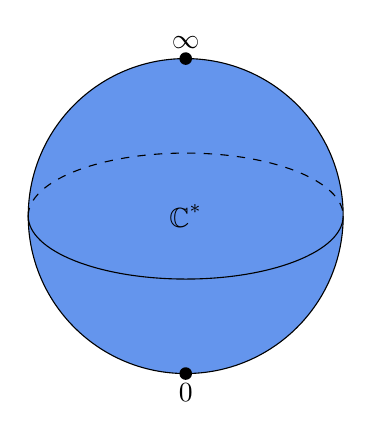
\begin{tikzpicture}[scale=2]

% Shade the open orbit C^*
\fill[CornflowerBlue] (0,0) circle (1);

% Draw sphere outline
\draw (0,0) circle (1);

% Draw equator
\draw (-1,0) arc (180:360:1 and 0.4);
\draw[dashed] (-1,0) arc (180:0:1 and 0.4);

% North pole (infinity)
\fill (0,1) circle (0.04);
\node[above] at (0,1) {$\infty$};

% South pole (0)
\fill (0,-1) circle (0.04);
\node[below] at (0,-1) {$0$};

% Label open orbit
\node at (0,0) {$\mathbb{C}^*$};

\end{tikzpicture}
\end{center}

For a $K$-equivariant perverse sheaf $\CF^{\bullet}$ on it, we calculate its characteristic cycle $\mathrm{CC}(\CF^{\bullet})$ use the formula

\[
\chi^{mic}_{S} = \sum_{S' > S} c(S,S') \chi^{loc}_{S'},
\]


only need to determine the coefficients $c(S,S') (= \sum_i (-1)^i H^i_c(J \cap S', K \cap S'; \BC))$ for $S' > S$, where $(J,K)$ is the normal Morse datum of S, which is well-defined up to homeomorphism.


\begin{itemize}
  \item For the open orbit $\BC^*$, we have $S' = \BC^*$ and $c(\BC^*,\BC^*) = -1$.
  \item For the closed orbit $\{0\}$, we have $S' = \{0\}, \BC^*$, and $c(\{0\},\{0\}) = 1$, for $c(\{0\},\BC^*)$, the pair $(J \cap S', K \cap S')$ is the following picture

\begin{center}
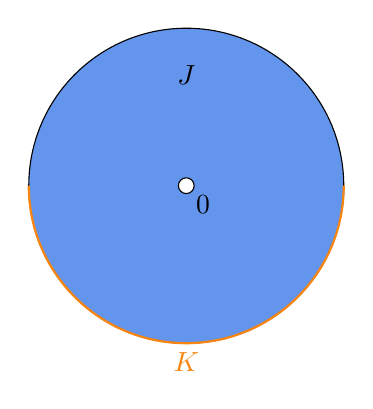
\begin{tikzpicture}[scale=2]

% Draw punctured disc (light fill)
\fill[CornflowerBlue] (0,0) circle (1);
\fill[white] (0,0) circle (0.05); % puncture at the origin

% Draw the boundary circle
\draw (0,0) circle (1);

% Draw the puncture as a hollow point
\draw (0,0) circle (0.05);
\node[below right] at (0,0) {$0$};

% Draw the lower half-cycle (closed subset K)
\draw[BurntOrange, thick] (1,0) arc (0:-180:1); % lower semicircle
\node[BurntOrange, below] at (0,-1) {$K$};

% Label the punctured disc
\node at (0,0.7) {$J$};

\end{tikzpicture}
\end{center}
therefore $c(\{0\},\BC^*) = \sum_i (-1)^i H^i_c(J \cap \BC^*, K \cap \BC^*; \BC) =^{?} -1$.
\end{itemize}


So we have

\begin{align*}
  \chi^{mic}_{0} &= \chi^{loc}_{0} - \chi^{loc}_{\BC^*}, \\ 
  \chi^{mic}_{\infty} &= \chi^{loc}_{\infty} - \chi^{loc}_{\BC^*}, \\
  \chi^{mic}_{\BC^*} &= -\chi^{loc}_{\BC^*}.
\end{align*}
 


\section{2026.3.22 Perverse sheaves on $\BC$}

Construuctible sheaves on $\BC = \BC^* \sqcup \{0\}$. Some calculations comes from the lecture notes by Geordie Williamson \cite{Wil15}.

Denote $j: \BC^* \hookrightarrow \BC$ the open inclusion, $i: \{0\} \hookrightarrow \BC$ the closed inclusion. Then we have the following six functors:
\[
\begin{tikzcd}[column sep=huge]
  D^b(\mathbb{C}^*) 
  \arrow[r, shift left=2.5ex, "j_!"]  
  \arrow[r, shift right=2.5ex, "j_*"'] 
  & D^b_c(\mathbb{C}) 
  \arrow[r, shift left=2.5ex, "i^*"] 
  \arrow[r, shift right=2.5ex, "i^!"']
  \arrow[l, "j^{*} = j^!" description] 
  & D^b(\{0\})
  \arrow[l, "i_* = i_!" description]
\end{tikzcd}
\]

$\CL$ is a local system on $\BC^*$. 

$j_!\CL$ has no quotient supported on $\{0\}$, $j_*$ has no subobject supported on $\{0\}$. $j_!\CL[1]$ and $j_*\CL[1]$ are perverse sheaves on $\BC$.


\begin{rk}
  Actually when $j: S \hookrightarrow  X$ is \colorbox{CornflowerBlue}{affine locally closed embedding} , $j_!$ and $j_*$ are $t$-exact for the perverse $t$-structure, so $j_!\CL[\dim S]$ and $j_*\CL[\dim S]$ are perverse sheaves on $X$.
\end{rk}
  



  



By easy calculation of group cohomology, we have:

\begin{align*}
  H^i(j_*\CL[1]_0) = \left\{
  \begin{array}{ll}
    0 & i \neq 0,-1 \\
    V_{\mu} & i = 0 \\
    V^{\mu} & i = -1
  \end{array}
  \right. 
\end{align*}

There is an exact sequence of perverse sheaves on $\BC$:
\[0 \to i_*V^{\mu} \to j_!\CL[1] \to j_*\CL[1] \to i_*V_{\mu} \to 0.\]






\section{2026.3.31 Enhanced flag variety and line bundles on $\CB$}
\noindent\textbf{\large I. The Enhanced Flag Variety and $G_0/N$ Isomorphism \cite{BB93}} 
\vspace{2mm}
\hrule 
\vspace{3mm}

$\fg$ be a complex semisimple Lie algebra, ${^{a}\fh} = \fb/[\fb,\fb]$ be the universal Cartan subalgebra, $G$ be the automorphism group of $\fg$, $G_0$ be the connected component of $G$, it is the adjoint group of $\fg$.

Attached to ${^{a}\fh}$ is a root system $\Delta$, and the Weyl group $W$. Although there isn't a well defined action of ${^{a}\fh} = \fb/[\fb,\fb]$ on $\fg/\fb = \fn^*$, the action of ${^{a}\fh}$ on $(\fn/[\fn,\fn])^*$ is well defined, and there is a canonical decomposition:
\[
  \left(\fn/[\fn,\fn]\right)^* = \bigoplus_{\alpha \in \Sigma} (\fn/[\fn,\fn])^*_{\alpha},
\]

Where $\Sigma$ is the set of simple roots. Note that this choice of positive root system is opposite to the one usually used in representation theory, but it is more natural in geometry since dominant implies positive line bundle in this way.

The enhanced flag variety $\tilde{\CB}$ is defined as the variety of pairs $(\fb, \{x_{\alpha}\}_{\alpha \in \Sigma})$ where $\fb$ is a Borel subalgebra of $\fg$, and $\xi$ is a nonzero element in $(\fn/[\fn,\fn])^*_{\alpha}$. There is a natural projection map $\pi : \tilde{\CB} \to \CB$ which forgets the second component, and is an $H$ principle bundle.

There is a $G$ action on $\tilde{\CB}$ defined by $g \cdot (\fb, \{x_{\alpha}\}_{\alpha \in \Sigma}) = (\Ad(g)\fb, \{\Ad^*(g)x_{\alpha}\}_{\alpha \in \Sigma})$. There is also an $H$ action on $\tilde{\CB}$ defined by $h \cdot (\fb, \{x_{\alpha}\}_{\alpha \in \Sigma}) = (\fb, \{\alpha(h)x_{\alpha}\}_{\alpha \in \Sigma})$. These two actions is compatible in the following way:
\[
  g \cdot h \cdot (\fb, \{x_{\alpha}\}_{\alpha \in \Sigma}) = \kappa_{g}(h) \cdot g \cdot (\fb, \{x_{\alpha}\}_{\alpha \in \Sigma}),
\]  

where $\kappa: G \to \mathrm{Aut}(H)$ is the action as outer automorphisms of $H$.

The adjoint group $G_0$ acts transitively on $\tilde{\CB}$, and the stabilizer of a base point $(\fb, \{x_{\alpha}\}_{\alpha \in \Sigma})$ is $N$. So we have an isomorphism $\tilde{\CB} \simeq G_0/N$. Under this identification, the $G$ action on $\tilde{\CB}$ is given by $g \cdot (g_0N) = gg_0(N)$, and the $H$ action on $\tilde{\CB}$ is given by $h \cdot (g_0N) = g_0 hN$.

\vspace{5mm}



\noindent\textbf{\large II. Line Bundles on $\CB$ and Very Ampleness}
\vspace{2mm}
\hrule 
\vspace{3mm}


Now $G$ is a connected reductive group.

\begin{lem}
  Let $G \to \GL(V)$ be a finite-dimensional representation of $G$, $k \cdot v \subseteq V$ be a one-dimensional subspace, $P = \mathrm{Stab}_G(k \cdot v)$. Suppose that $k_{\lambda}$ be the one-dimensional representation of $P$ defined by the action of $P$ on $k \cdot v$, then $i^*(\CO_{\BP(V)}(1)) = \CO_{G/P}(\lambda)$.
\end{lem}

\begin{proof}
  Note that $\CO_{\BP(V)}(-1)$ is the tautological line bundle, $P$ action on the fiber of $\CO_{\BP(V)}(-1)$ at $k \cdot v$ is given by $k_{\lambda}$. So $k_{-\lambda}$ for $\CO(1)$, also note that $\CO_{G/P}(\lambda) = G \times^{P} k_{-\lambda}$.
\end{proof}

\begin{lem}
  $\CO_{\CB}(\lambda)$ is very ample if and only if $\lambda$ is regular dominant ($\lambda \in X^+(H)$).
\end{lem}

\begin{proof}
  Consider the Verma module $V^{\lambda} = \CU(\fg) \otimes_{\CU(\fh)} k_{\lambda}$. By the transitive group action of $G$ on $\CB$, $\CO(\lambda)$ is generated by global sections $\Gamma(\CB,\CO(\lambda)) = V^{\lambda}$. Hence there is a surjection $\Gamma(\CB,\CO(\lambda)) \twoheadrightarrow \CO(\lambda) \otimes_k k_{eB} = k_{\lambda}$. Taking dual, we have $k_{-\lambda} \hookrightarrow (V^{\lambda})^*$.
  
  Since $\lambda$ is regular dominant, the stablizer of $k_{-\lambda}$ in $(V^{\lambda})^*$ is the Borel $B$, by the previous lemma, we have a $G$-equivariant morphism $\CB \hookrightarrow \BP((V^{\lambda})^*)$ such that $\CO(\lambda)$ is the pullback of $\CO(1)$, hence $\CO(\lambda)$ is very ample.
\end{proof}





\section{2026.4.5 Tangent map of the projection $G \times^P V \to V$}
$G$ is a compex algebraic group, $P$ is a closed subgroup of $G$ with a finite dimensional rational representation $V$. suppose that $\fg = \fu \oplus \fp$.

\[
  \begin{tikzcd}
    Y = G \times^P V \arrow[r, "\pi"] \arrow[d] & V \\
    G/P & 
  \end{tikzcd}
\]

There is an isomorphism:

\[
  \fu \oplus V \xrightarrow{\sim} T_{\bar{(1,\alpha)}}(G \times^P V)  ,
\]
which sends $(u,v)$ to $u^{\sharp} + v$, where $v \in V$ is regarded as a tangent vector of the fiber $V$ at $\alpha$, and $u^{\sharp}$ is the vector field on $Y$ generated by the action of $u \in \fu \subset \fg$.
 
The tangent map of $\pi$ at $\bar{(1,\alpha)}$ is:
\begin{align*}
  d \pi_{\bar{(1,\alpha)}} &: \fu \oplus V \to T_{\bar{(1,\alpha)}}(G \times^P V) \to V, \\
  d\pi_{\bar{(1,\alpha)}}(u,v) &= u \cdot \alpha + v,
\end{align*}
since $\pi(g,\alpha) = g \cdot \alpha$.

The above calculation is instrumental in extending the Kostant-Kirillov symplectic form of nilpotent orbits to the Jacobson-Morozov resolution of a nilpotent orbit:
\[
\begin{tikzcd}
  G \times^P \fg_{\geq 2} \arrow[r, "\pi"] & \bar{\BO} \\
  G \times^{P}  P \cdot e = G/Z_P(e) \arrow[r] \arrow[u,hookrightarrow ] & \BO \arrow[u,hookrightarrow ] 
\end{tikzcd}
\]

\[
  \pi^* \omega_{KK,\alpha}((u,v),(x,y)) = \kappa(\alpha, [u,x]) + \kappa(u,y) - \kappa(v,x).
\]
Where $(u,v), (x,y) \in \fg_{\leq -1} \oplus \fg_{\geq 2} = T_{\bar{(1,\alpha)}}(G \times^P \fg_{\geq 2})$.

This 2-form can be extended to a $G$-invariant 2-form $\omega_Y$ on $G \times^P \fg_{\geq 2}$. 

It is easy to check that $\mathrm{Rad}(\omega_{Y}) = \fg_{-1} \oplus 0$, so this form is symplectic if and only if $\fg_{-1} = 0$, which is equivalent to the nilpotent orbit $\BO$ is even.

\section{2026.4.22 Symplectic Form and Moment map}

\cite{Losev2022Topics}
\subsection{Examples of Symplectic Form and Moment map}

\begin{prop}
  The Kostant-Kirillov form $\omega_{KK}$ on a coadjoint orbit $\BO$ is closed and hence symplectic.
\end{prop}

\begin{proof}
  For $X \in \fg$ we have a vector field $X^{\sharp}$ on $\BO$ defined by 
  \[
    \boxed{\displaystyle X^{\sharp}_{\alpha} = \frac{\dd}{\dd t} \bigg|_{t=0} \Ad^*(\exp(tX))\alpha = [X,\alpha]}
  \]
  
  Define a smooth function $f_{X} = \kappa \bra{-,X}$ on $\BO$, then we have
  \[  \dd f_{X}(Y^{\sharp}) = \kappa([Y,\alpha],X) = \kappa(\alpha,[X,Y]) = \omega_{KK}(X^{\sharp},Y^{\sharp}). \]
  So $\iota_{X^{\sharp}} \omega_{KK} = df_{X}$.

  By Cartan's magic formula, we have
  \[  \CL_{X^{\sharp}} \omega_{KK} = \dd \iota_{X^{\sharp}} \omega_{KK} + \iota_{X^{\sharp}} \dd \omega_{KK} = \dd \dd f_{X} + \iota_{X^{\sharp}} \dd \omega_{KK} = \iota_{X^{\sharp}} \dd \omega_{KK}. \]
  Since $\omega_{KK}$ is $G$-invariant, $\CL_{X^{\sharp}} \omega_{KK} = 0$, hence $\iota_{X^{\sharp}} \dd \omega_{KK} = 0$ for all $X \in \fg$. Since the vector fields $X^{\sharp}$ span the tangent space of $\BO$ at each point, we have $\dd \omega_{KK} = 0$.
\end{proof}



Now, we cansider the simplest example of Hamiltonian $G$-space. 

Let $(V,\omega)$ be a complex symplectic space, and $G = \Sp(V,\omega)$

\begin{prop}
  The moment map $\mu : V \to \fg^*$ is given by $\bra{\mu(v),X} = \frac{1}{2}\omega(Xv,v)$ for $v \in V$ and $X \in \fg$.
\end{prop}

\begin{proof}
  Set $H_X(v) = \bra{\mu(v),X}$, we only need to check that $\iota_{X^{\sharp}} \omega = \dd H_X$:
  \begin{align*}
    (\dd H_X)_{v}(\delta v) &= \frac{1}{2} \omega(X \delta v, v) + \frac{1}{2} \omega(Xv, \delta v) \\
    &= \omega(Xv, \delta v) \\
    &= (\iota_{X^{\sharp}} \omega )_{v}(\delta v).
  \end{align*}
  Where $\delta v$ is a tangent vector of $V$ at $v$, which can be identified with an element in $V$ itself.
\end{proof}

\begin{rk}
  Note that $X^{\sharp}(v) = X \cdot v$ for $v \in V$.
\end{rk}

\begin{lem}
  The symplectic group $G$ acts transitively on $V \backslash \Bra{0}$.
\end{lem}

\begin{proof}
  Use induction on the dimension.
\end{proof}


\begin{prop}
  The moment map $\mu: V \backslash \Bra{0} \to \fg^*$ is a double cover onto the minimal nilpotent orbit $\BO_{min}$ in $\fg^*$.
\end{prop}

\begin{proof}
  Use trace form on $\fg$ to identify $\fg$ with $\fg^*$, then we can check that $\mu(v) = (u \mapsto \omega(v,u)v) \in \fg$.
  $\mu(v)$ is nilpotent since $\mu(v)^2 = 0$, and the image of $\mu$ is a nonzero nilpotent orbit. It is the minimal nilpotent orbit since $\mu(v)$ has rank $1$. $G$ acts transitively on $V \backslash \Bra{0}$, $\mu$ is a double cover onto $\BO_{min}$.
\end{proof}

\begin{rk}
  $\BO_{min} = \sqbra{2,1, \cdots,1}$ and $\pi_{1}^{G}(\BO_{\min}) = \BZ/2\BZ$, the cover above is the universial cover of $\BO_{min}$.
\end{rk}



\subsection{Classical and Quantum Fromal Darboux Theorems}

The classical Darboux theorem states that every point in a symplectic manifold has a neighborhood that is symplectomorphic to an open subset of the standard symplectic vector space. Here we investigate a formal algebraic analog of this theorem and its extension to quantization.

\begin{lem}
  Let $A$ be a Poisson algebra and $\fm$ be its maximal ideal with $A/\fm = \BC$. Then the Poisson bracket on $A$ induces a skew-symmetric form on $\fm/\fm^2$.
\end{lem}

\begin{proof}
  Define the skew-symmetric form as:
  \[
    \omega(a + \fm^2, b + \fm^2) = \{a,b\} \mod \fm.
  \]
\end{proof}

Now let $A = \mathbb{C}[[x_1, \dots, x_{2n}]]$ so that there is a unique maximal ideal $\fm = (x_1, \dots, x_{2n})$ and $\fm/\fm^2$ is spanned by $x_i + \fm^2$. Suppose that the Poisson bracket on $A$ induces a non-degenerate skew-symmetric form on $\fm/\fm^2$. So $\{x_i, x_j\} = \omega_{ij} \mod \fm$ for some $\omega_{ij} \in \BC$, then the matrix $(\omega_{ij})$ is non-degenerate skew symmetric.

\begin{thm}[Formal Darboux Theorem]
   There exists a formal change of coordinates $y_i = y_i(x_1, \dots, x_{2n}) \in \fm$ such that $\{y_i, y_j\} = \omega_{ij} \in \BC$.
\end{thm}

\begin{proof}
  Use induction, suppose that we have found $x_{i}^{\bra{n}} \in \fm$ such that $\Bra{x_{i}^{\bra{n}}, x_{j}^{\bra{n}}} \equiv \omega_{ij} \mod \fm^n$ (i.e. $\Bra{x_i^{(n)}, x_j^{(n)}} = \omega_{ij} + R_{ij}^{(n)} $ for some $R_{ij}^{(n)} \in \fm^n$). We want to find $\delta_i^{\bra{n}} \in \fm^{n+1}$ such that $\Bra{x_i^{\bra{n}} + \delta_i^{\bra{n}}, x_j^{\bra{n}} + \delta_j^{\bra{n}}} \equiv \omega_{ij} \mod \fm^{n+1}$.
  
  Since 
  \begin{align*}
    \Bra{x_i^{(n)} + \delta_i^{(n)}, x_j^{(n)} + \delta_j^{(n)}} &= \Bra{x_i^{(n)}, x_j^{(n)}} + \Bra{\delta_i^{(n)}, x_j^{(n)}} + \Bra{x_i^{(n)}, \delta_j^{(n)}} + \Bra{\delta_i^{(n)}, \delta_j^{(n)}} \\
    &\equiv \Bra{x_i^{(n)}, x_j^{(n)}} + \Bra{\delta_i^{(n)}, x_j^{(n)}} + \Bra{x_i^{(n)}, \delta_j^{(n)}} \mod \fm^{n+1}\\
    &\equiv \omega_{ij} + R_{ij}^{(n)} + \Bra{x_i^{(n)}, \delta_j^{(n)}} - \Bra{ x_j^{(n)}, \delta_i^{(n)}} \mod \fm^{n+1}.
  \end{align*}
  We need to solve the following equation for $\delta_i^{(n)}$:
  \[\Bra{x_i^{(n)}, \delta_j^{(n)}} - \Bra{ x_j^{(n)}, \delta_i^{(n)}} = -R_{ij}^{(n)} \mod \fm^{n+1}.\]
  
  Note that $\Bra{x_i^{(n)}, \delta_j^{(n)}} - \Bra{ x_j^{(n)}, \delta_i^{(n)}} = \omega_{ik}x_k^{(n)}\frac{\partial \delta_j^{(n)}}{\partial x_k} - \omega_{jk}x_k^{(n)}\frac{\partial \delta_i^{(n)}}{\partial x_k}$, we can solve the above equation by setting 
  $$\delta_i^{(n)} = -\frac{1}{n+1} \sum_{k,l} \omega^{kl} x_k^{(n)} R_{li}^{(n)}.$$
  
  Set $x_i^{(n+1)} = x_i^{(n)} + \delta_i^{(n)}$, then $y_i = \lim_{n \to \infty} x_i^{(n)}$ satisfies $\{y_i, y_j\} \in \BC$.
\end{proof}


\begin{thm}[Quantum Formal Darboux Theorem]
  Let $\CA_{\hbar}$ be a formal quantization of the Poisson algebra $A$. Then there are elements $\hat{y_i} \in \CA_{\hbar}$ such that
  \begin{itemize}
    \item $\hat{y_i} \equiv x_i \mod \hbar \CA_{\hbar}$;
    \item $\frac{1}{\hbar}\left[\hat{y_i}, \hat{y_j}\right] \in \BC$.
  \end{itemize}
\end{thm}

\begin{proof}
  Choose lift of $y_i$ in $\CA_{\hbar}$, denoted by $\hat{y_i}^{(1)}$. Then $\frac{1}{\hbar}\left[\hat{y_i}^{(1)}, \hat{y_j}^{(1)}\right] \equiv \{y_i, y_j\} = \omega_{ij} \mod \hbar$, so we can write $\frac{1}{\hbar}\left[\hat{y_i}^{(1)}, \hat{y_j}^{(1)}\right] = \omega_{ij} + \hbar R_{ij}^{(1)}$ for some $R_{ij}^{(1)} \in \CA_{\hbar}$ and $\omega_{ij} \in \BC$.

  Again, use induction, suppose that we have found $\hat{y}_i^{(n)}$ lift $y_i$ such that $\frac{1}{\hbar}\left[\hat{y}_i^{(n)}, \hat{y}_j^{(n)}\right] = \omega_{ij} + \hbar^{n} R_{ij}^{(n)}$ for some $R_{ij}^{(n)} \in \CA_{\hbar}$, we want to find $\delta_i^{(n)} \in \hbar^{n+1} \CA_{\hbar}$ such that $\frac{1}{\hbar}\left[\hat{y}_i^{(n)} + \delta_i^{(n)}, \hat{y}_j^{(n)} + \delta_j^{(n)}\right] = \omega_{ij} + \hbar^{n+1} R_{ij}^{(n+1)}$.

  This is equivalent to solving the following equation for $\delta_i^{(n)}$:
  \[\frac{1}{\hbar}\left[\hat{y}_i^{(n)}, \delta_j^{(n)}\right] - \frac{1}{\hbar}\left[\hat{y}_j^{(n)}, \delta_i^{(n)}\right] = -\hbar^{n} R_{ij}^{(n)} \mod \hbar^{n+1}.\]
  Note that $\frac{1}{\hbar}\left[\hat{y}_i^{(n)}, \delta_j^{(n)}\right] - \frac{1}{\hbar}\left[\hat{y}_j^{(n)}, \delta_i^{(n)}\right] = \omega_{ik} \hat{y}_k^{(n)}\frac{\partial \delta_j^{(n)}}{\partial \hat{y}_k} - \omega_{jk} \hat{y}_k^{(n)}\frac{\partial \delta_i^{(n)}}{\partial \hat{y}_k}$, we can solve the above equation by setting
$$\delta_i^{(n)} = -\frac{1}{n+1} \sum_{k,l} \omega^{kl} \hat{y}_k^{(n)} R_{li}^{(n)}.$$
  
  Set $\hat{y}_i^{(n+1)} = \hat{y}_i^{(n)} + \delta_i^{(n)}$, then $\hat{y}_i = \lim_{n \to \infty} \hat{y}_i^{(n)}$ satisfies $\frac{1}{\hbar}\left[\hat{y}_i, \hat{y}_j\right] = \omega_{ij} \in \BC$.
\end{proof}


\subsection{Localness of Differential Operators}

\aiblock{
  Any differential operator on $A$ can extend to localizations and completions.
  \begin{itemize}
    \item Extension to the Localization $S^{-1}A$. Let $A$ be a commutative algebra over a field $k$. A $k$-linear map $L: A \to A$ is a differential operator of order $\le k$ if for any $a_0, \dots, a_k \in A$, the iterated commutator vanishes:$$[\dots[[L, a_0], a_1], \dots, a_k] = 0$$where $[L, a](b) = L(ab) - aL(b)$. We denote the space of such operators as $\text{Diff}^k(A)$.The General Extension FormulaFor any $L \in \text{Diff}^k(A)$, the unique extension $\widetilde{L} \in \text{Diff}^k(S^{-1}A)$ is determined by its action on the reciprocal of an element $s \in S$. The formula uses the iterated adjoint action $\text{ad}_s(L) = [L, s]$:$$\widetilde{L}\left(\frac{1}{s}\right) = \sum_{j=0}^{k} (-1)^j s^{-(j+1)} \text{ad}_s^j(L)(1)$$Applying this to a general fraction $\frac{a}{s}$ via the Leibniz-like property for higher-order operators, we get:$$\widetilde{L}\left(\frac{a}{s}\right) = \sum_{j=0}^{k} (-1)^j s^{-(j+1)} \text{ad}_s^j(L)(a).$$
    \item Specific Cases for Low OrderOrder 0 (Multiplication by $f \in A$):$$\widetilde{L}\left(\frac{a}{s}\right) = s^{-1}(f \cdot a) = \frac{fa}{s}$$Order 1 (Derivations, where $L(1)=0$):Using the general formula for $j=0, 1$:$$\widetilde{L}\left(\frac{a}{s}\right) = s^{-1}L(a) - s^{-2}[L, s](a) = \frac{L(a)}{s} - \frac{L(sa) - sL(a)}{s^2} = \frac{sL(a) - aL(s)}{s^2}$$Order 2 (e.g., a Laplacian $\Delta$):$$\widetilde{L}\left(\frac{a}{s}\right) = \frac{\Delta(a)}{s} - \frac{\Delta(sa)-s\Delta(a)}{s^2} + \frac{\Delta(s^2 a) - 2s\Delta(sa) + s^2\Delta(a)}{s^3}.$$
    \item Extension to the Completion $\widehat{A}$. Let $I \subset A$ be an ideal. The completion is the inverse limit $\widehat{A} = \varprojlim A/I^n$.The Continuity PrecisionA differential operator $L$ of order $k$ is stricly continuous with respect to the $I$-adic topology because it satisfies:$$L(I^n) \subseteq I^{n-k} \quad \text{for all } n \ge k$$This filtration ensures that for any Cauchy sequence $(a_n)$ in $A$, the sequence $(L(a_n))$ is also Cauchy in the $I$-adic sense. The extension $\widehat{L}: \widehat{A} \to \widehat{A}$ is defined by taking the limit of the action on the truncated sequences:$$\widehat{L}\left( \lim_{n \to \infty} a_n \right) = \lim_{n \to \infty} L(a_n)$$Because $L$ is a polynomial-type operator (it "sees" only a finite neighborhood of any point algebraically), this limit is always well-defined and unique.
    \item The Poisson Bracket CaseA Poisson bracket $\{ \cdot, \cdot \}$ is a bilinear map that is a derivation (order 1 operator) in each slot.On $S^{-1}A$: Since $L_f = \{f, \cdot\}$ is a derivation, the extension is forced by the first-order formula derived above. For $a/s, b/t \in S^{-1}A$:$$\left\{ \frac{a}{s}, \frac{b}{t} \right\} = \frac{1}{s^2 t^2} \left( st\{a, b\} - at\{s, b\} - bs\{a, t\} + ab\{s, t\} \right)$$On $\widehat{A}$: Since the bracket is a derivation in each variable, it is continuous in each variable. By the universal property of completions of bilinear maps, it extends uniquely:$$\{ \hat{a}, \hat{b} \}_{\widehat{A}} = \lim_{n \to \infty} \{ a_n, b_n \}_A$$This ensures that $\widehat{A}$ inherits the Poisson algebra structure from $A$ without any ambiguity.
  \end{itemize}
  }





\section{2026.4.24 Normality of Nilpotent Orbits}

\textbf{Normality of Closure of Nilpotent Orbits}

\begin{thm}[Main theorem]
  For a nilpotent otbit $\BO$ in a complex semisimple Lie algebra $\fg$, its closure $\bar{\BO}$ is normal if and only if $\BC[\BO] = \BC[\bar{\BO}]$.
\end{thm}

\begin{lem}[Serre's criterion for normality]
  A is a commutative Noetherian ring. Then $A$ is normal if and only if it satisfies the following two conditions:
\begin{itemize}
  \item [($R_1$)] For any prime ideal $\fp$ of $A$ with $\mathrm{ht}(\fp) \leq 1$, the localization $A_{\fp}$ is a regular local ring.
  \item [($S_2$)] For any prime ideal $\fp$ of $A$, we have $\mathrm{depth}(A_{\fp}) \geq \min\{2, \mathrm{ht}(\fp)\}$.
\end{itemize}
\end{lem}

\begin{proof}[Proof of Main Theorem]
  ($\Rightarrow$) If $\bar{\BO}$ is normal, then by Serre's criterion, we get infromation about the depth inequality, and then we can apply the algebraic Hartogs theorem \cite[Chapter III, Exercise 3.5]{Har77} to conclude that $\BC[\BO] = \BC[\bar{\BO}]$.

  ($\Leftarrow$) If $\BC[\BO] = \BC[\bar{\BO}]$, then $\BC[\bar{\BO}]$ is a domain and integrally closed in its field of fractions, Since $\BC[\BO]$ is smooth. Hence $\BC[\bar{\BO}]$ is normal.
\end{proof}



\section{2026.4.25 Filtered Quantization of Nilcone}

\cite{Losev2022Topics}

\begin{lem}
  Let $A$ be a filtered algebra, $I \subseteq A$ an ideal, we have a short exact sequence:
  \[
    0 \to \gr I \to \gr A \to \gr (A/I) \to 0.
  \]
\end{lem}

\begin{proof}
  $I$ has an induced filtration $I_{\leq n} = I \cap A_{\leq n}$, and $\gr I = \bigoplus_{n} I_{\leq n}/I_{\leq n-1}$ is a graded ideal of $\gr A$. It is easy to see that the map $\gr A \to \gr (A/I)$ is surjective, and $\gr I \to \gr A$ is injective. For an element $a + A_{\leq i-1} \in \gr_{i} A$, then
  \begin{align*}
    &a + A_{\leq i-1} \mapsto 0 \in \gr_{i}(A/I) \\
    \Leftrightarrow \quad  &\bar{a} \in (A/I)_{\leq i-1} \\
    \Leftrightarrow \quad  &\exists \ a' \in A_{\leq i-1} \text{ such that } a - a' \in I \\
    \Leftrightarrow \quad  &a + A_{\leq i-1} \in I_{\leq i}/I_{\leq i-1}.
  \end{align*}
\end{proof}

\begin{rk}
  If $I = \langle f_1, \cdots , f_n\rangle$, then $\langle\sigma(f_1),\cdots,\sigma(f_n)\rangle \subseteq \gr I$.
\end{rk}  

\begin{prop}
  $A$ is a $\BZ_{\geq0}$ graded Noetherian Poisson algebra with $\deg \Bra{,} = -d < 0$, $\CA$ is its filtered quantization, and $\CI = \langle \hat{f_1}, \cdots, \hat{f_n}  \rangle$ ($\hat{f}_i \in \CA_{d_i}$), $f_i = \hat{F_i} + \CA_{\leq d_i -1}$, with the following conditions:
\begin{itemize} 
  \item $f_1, \cdots, f_n$ is a regular sequence in $A$;
  \item $\sqbra{\hat{f}_i, \hat{f}_j} = \sum_{i = 1}^{r} \hat{c}_{ij}^k \hat{f}_k$, with $\hat{c}_{ij}^k  \in \CA_{\leq d_i + d_j -d -d_k}$.
\end{itemize}
Then $\gr \CI = \langle f_1, \cdots, f_n\rangle$.
\end{prop}
  

\begin{proof}
  We only need to check that $\gr \CI \subseteq \langle f_1, \cdots, f_n\rangle$. Assume on the contrary that there exists a positive integer $e$ and $\hat{b}_i \in \CA_{\leq e-d_i}$ such that $\sigma(\sum_{i=1}^{n} \hat{b}_i \hat{f}_i) \notin \langle f_1, \cdots, f_n\rangle$. Also assume $e$ is the smallest integer with this property.
  
  Note that $\sum_{i=1}^{n} b_i f_i \in A_{e}$ must be zero, otherwise $\sigma(\sum_{i=1}^{n} \hat{b}_i \hat{f}_i) = \sum_{i=1}^{n} b_i f_i \in \langle f_1, \cdots, f_n\rangle$. So by the vanishing of the first Koszul homology, we can find $b_{ij} \in A$ such that $b_i = \sum_{j=1}^{n} b_{ij} f_j$ and $b_{ij} = -b_{ji}$ for $i \neq j$. By restriction to the degree $d_i$ we can assume that $b_{ij} \in A_{\leq e-d_i - d_j}$, take lifts $\hat{b}_{ij} \in \CA_{\leq e-d_i - d_j}$, such that $\hat{b}_{ij} = -\hat{b}_{ji}$. Then $\hat{b}'_i := \hat{b}_i - \sum_{j=1}^{n} \hat{b}_{ij} \hat{f}_j \in \CA_{< e - d_i}$.
  \begin{align*}
    \sum_{i=1}^{n} \hat{b}_i \hat{f}_i &= \sum_{i=1}^{n} \hat{b}'_i \hat{f}_i + \sum_{i,j=1}^{n} \hat{b}_{ij} \hat{f}_j \hat{f}_i \\
    &= \sum_{i=1}^{n} \hat{b}'_i \hat{f}_i +  \sum_{j < k} \hat{b}_{jk} [\hat{f}_j, \hat{f}_k] \\
    &= \sum_{i=1}^{n} \hat{b}'_i \hat{f}_i +  \sum_{j < k} \hat{b}_{jk} \sum_{i = 1}^{n} \hat{c}_{jk}^i \hat{f}_i \\
    &= \sum_{i=1}^{n} \left( \hat{b}'_i + \sum_{j < k} \hat{b}_{jk} \hat{c}_{jk}^i \right) \hat{f}_i.
  \end{align*}
  But $\hat{b}'_i + \sum_{j < k} \hat{b}_{jk} \hat{c}_{jk}^i \in \CA_{< e - d_i}$, which is a contradiction to the minimality of $e$.
\end{proof}


A discovery: Harish-Chandra's isomorphism can be viewed as a quantized version of the Chevalley restriction theorem.

\begin{thm}[Chevalley restriction theorem]
  Let $\fg$ be a complex reductive Lie algebra, $\fh$ be a Cartan subalgebra, $W$ be the Weyl group. Then the restriction map $\BC[\fg]^G \to \BC[\fh]^W$ is an isomorphism.
\end{thm}

\begin{thm}[Harish-Chandra isomorphism]
  Let $\fg$ be a complex reductive Lie algebra, $\fh$ be a Cartan subalgebra, $W$ be the Weyl group. Then there is an isomorphism $Z(\fg) = \CU(\fg)^{G} \to \BC[\fh]^W$.
\end{thm}

\begin{cor}
  $\fh/W$ parametrizes both the filtered Poisson deformations and the filtered quantizations of $\CN$.
\end{cor}



Some phenomena of separation of variables:
\begin{itemize}
  \item $\BC[\fg] = \BC[\fg]^G \otimes_{\BC} \CH$;
  \item $\BC[\fh] = \BC[\fh]^W \otimes_{\BC} \CH$;
  \item $\BC[V] = \BC[V]^{\SO(V)} \otimes_{\BC} \CH(V) = \BC[r^2] \otimes_{\BC} \CH(V)$. (Spherical harmonics)
\end{itemize}

\begin{proof}[Proof of the first separation of variables]
  There is an isomorphism $\BC[\fg] = \BC[\fg]^G_{+}\BC[\fg] \oplus \CH$.

  Choose a homogeneous vector space basis $\bar{b}_i$ of $\BC[\fg]/(\BC[\fg]^G_{+}\BC[\fg])$, and let $b_i$ be a homogeneous lift of $\bar{b}_i$ in $\CH$. Then $b_i$ is a vector space basis of $\CH$. By graded Nakayama's lemma, $b_i$ generates $\BC[\fg]$ as a $\BC[\fg]^G$-module, we claim that $b_i$ is a free basis of $\BC[\fg]$ as a $\BC[\fg]^G$-module, so that the following is an isomorphism
  \[
    \BC[\fg]^G \otimes_{\BC} \CH \to \BC[\fg], \quad f \otimes b \mapsto f b.
  \]

  If not, then there exists $r_i \in \BC[\fg]^G$ such that $\sum_{i} r_i b_i = 0$, and not all $r_i$ are zero. Projection to $\CH$ we have $\sum_{i} \bar{r}_i \bar{b}_i = 0$, since $\bar{b}_i$ is a vector space basis, so $\bar{r}_i = 0$ for all $i$ which means $r_i \in \BC[\fg]^G_{+}\BC[\fg] = \langle f_1, \cdots, f_n \rangle$, assume that $r_i = \sum_{j} r_{ij} f_j$ then
  \[
    0 = \sum_{i} r_i b_i = \sum_{i,j} r_{ij} f_j b_i = \sum_{j} f_j \underbrace{\left( \sum_{i} r_{ij} b_i \right)}_{a_j}.
  \]
  Since $f_i$ form a regular sequence, the first Koszul homology vanishes, which means that there exists $s_{jk}$ such that $a_j = \sum_{k} s_{jk} f_k $ and $s_{jk} = -s_{kj} \in \BC[\fg]$. So we have
  \[
    \sum_{k} s_{jk} f_k = a_j = \sum_{i} r_{ij} b_i.
  \]
  This implies that $r_{ij} \in \langle f_1, \cdots, f_n \rangle$, suppose $r_{ij} = \sum_{k} r_{ijk} f_k$, then
  \[
    0 = \sum_{i,j} r_{ij} f_j b_i = \sum_{i,j,k} r_{ijk} f_k f_j b_i = \sum_{j,k} f_j f_k \underbrace{\left( \sum_{i} r_{ijk} b_i \right)}_{a_{jk}}.
  \]
  Again by the vanishing of the second Koszul homology, there exists $s_{jkl}$ such that $a_{jk} = \sum_{l} s_{jkl} f_l$ and $s_{jkl} = -s_{jlk}$, so we have
  \[
    \sum_{l} s_{jkl} f_l = a_{jk} = \sum_{i} r_{ijk} b_i.
  \]
  This implies that $r_{ijk} \in \langle f_1, \cdots, f_n \rangle$, and we can continue this process to conclude that $r_i \in \langle f_1, \cdots, f_n \rangle^m$ for all $m$, which implies that $r_i = 0$.
\end{proof}








\section{2026.4.26 Divisors and Picard Groups}


Some relations between Picard groups, Cartier divisors, and Weil divisors.

$\mathrm{Pic}$ is the group of isomorphism classes of line bundles. $\mathrm{Cl}$ is the group of Weil divisors modulo linear equivalence. $\mathrm{CaCl}$ is the group of Cartier divisors modulo linear equivalence.

\begin{itemize}
  \item If $X$ is integral, then $\mathrm{Pic}(X) \cong \mathrm{CaCl}(X)$.
  \item If $X$ is integral and normal, then $\mathrm{Pic}(X) \hookrightarrow  \mathrm{Cl}(X)$.
  \item If $X$ is integral and locally factorial/Smooth, then $\mathrm{Pic}(X) \cong \mathrm{Cl}(X)$.
\end{itemize}

If $X$ is integral and normal, by Serre's criterion for normality, the singular locus of $X$ has codimension at least 2, hence $\mathrm{Cl}(X) \cong \mathrm{Cl}(X^{reg}) \cong \mathrm{Pic}(X^{reg})$. 

\section{2026.4.27 Symplectic Leaves of Nilpotent Orbits}

\cite{Losev2022Topics}

We prove that for a nilpotent orbit $\BO$ in a complex semisimple Lie algebra $\fg$,
\[
  \bar{\BO}^{reg} = \BO.
\]

\begin{lem}
  $\bar{\BO}^{reg}$ is symplectic.
\end{lem}

\begin{proof}
  Since $\bar{\BO}$ is Poisson, it has a Poisson bivector field $\pi \in \Gamma(\bar{\BO}, \wedge^2 T_{\bar{\BO}})$, and $\pi$ is non-degenerate on $\BO$, and we know that the zero locus of a section of a line bundle on the smooth variety $\bar{\BO}^{reg}$ has codimension at most 1, but $\mathrm{codim}_{\bar{\BO}^{reg}}(\{ \pi = 0 \}) \geq 2$, so $\pi$ is non-vanishing on $\bar{\BO}^{reg}$.
\end{proof}

Let $X$ be a Poisson variety, and $X_1 = X \backslash X^{reg}$, $X_{k+1} = X_k \backslash X_k^{reg}$. We say that $X$ has finitely many symplectic leaves if each $X_k^{reg}$ is symplectic. For a symplectic leaf, we mean an irreducible (connected) component of $X_k^{reg}$ for some $k$.

\begin{lem}
  Symplectic leaves are one one correspondence with prime Poisson ideals of $\BC[X]$.
\end{lem}

\begin{lem}
  $\bar{\BO}$ has finitely many symplectic leaves, and the symplectic leaves are exactly the nilpotent orbits contained in $\bar{\BO}$.
\end{lem}

\begin{proof}
  The second statement is due to the fact that Poisson bracket is generated by Lie bracket.
\end{proof}

\begin{lem}
  A smooth symplectic variety has no proper Poisson subvarieties, hence it is a symplectic leaf.
\end{lem}

\begin{proof}
  Suppose $X$ is a smooth symplectic variety, and let $x \in X$ be a point. 
  $$T_x X \xrightarrow{\pi_x} T_x^* X$$
  is an isomorphism.

  Under this isomorphism $H_f$ corresponds to $\dd f$, so we can see that $\mathrm{span}\set{H_f}{f \in \BC[X]} = T_x X$, but Poisson subvariety must tangent to all Hamiltonian vector fields, so it must be the whole $X$.
\end{proof}


\begin{proof}[Proof of $\bar{\BO}^{reg} = \BO$]
  Since $\bar{\BO}$ has finitely many symplectic leaves, $\bar{\BO}^{reg}$ is a symplectic leaf, hence it is a nilpotent orbit. Since $\BO \subseteq \bar{\BO}^{reg}$, we have $\bar{\BO}^{reg} = \BO$.
\end{proof}



\begin{rk}
  The argument above works for any coadjoint orbits in a complex Lie algebra, not necessarily semisimple.
\end{rk}



\begin{rk}
  For a nilpotent orbit cover $\tilde{\BO}$, we have a finite surjective morphism
  \[
    \pi: \mathrm{Spec}(\BC[\tilde{\BO}]) \to \bar{\BO},
  \]
  $\mathrm{Spec}(\BC[\tilde{\BO}])$ has finitely many symplectic leaves, and we also know that $\mathrm{Spec}(\BC[\tilde{\BO}])^{reg}$ is symplectic, it has no proper Poisson subvarieties, hence it is a symplectic leaf. By in this situation, symplectic leaves are not in one one correspondence with $G$-orbits any more, so $\tilde{\BO}$ may properly contained in $\mathrm{Spec}(\BC[\tilde{\BO}])^{reg}$.

  Actually in the case of exceptional Lie algebras, there exist some nilpotent orbits $\BO$ such that $\mathrm{codim}_{\bar{\BO}}(\bar{\BO} \backslash \BO) = 2$ but $\mathrm{codim}_{X}(X \backslash X^{reg}) \geq 4$, where $X = \mathrm{Spec}(\BC[\BO])$.
\end{rk}


\section{2026.4.27 Richardson Orbits and Symplectic Resolutions}

\subsection{A fundamental fact I often forget}

$G$ be a complex connected reductive algebraic, $\CB$ be the flag variety of $G$, then

\[
  T\CB = \set{(b,\xi)}{b \in \CB , \quad \xi \in \fg/b}.
\]

For any $X \in \fg$, the vector field $X^{\sharp}$ on $\CB$ generated by $X$-action is given by

\[
  X^{\sharp}(b) = (b, X + b).
\]

We also have the cotangent bundle
\[
  T^*\CB = \set{(b, \xi)}{b \in \CB, \quad \xi \in b^{\perp} \subseteq \fg^*}.
\]

For a symmetric subgroup $K$ of $G$, we have:

\[
  T^*_{K} \CB = \set{(b, \xi)}{b \in \CB, \quad \xi \in b^{\perp} \cap \fk^{\perp}}.
\]

We have the following Cartersian diagram:
\[
  \begin{tikzcd}
    T^*_{K} \CB \arrow[r, hook] \arrow[d] & T^* \CB \arrow[d] \\
    \fk^{\perp} \arrow[r, hook] & \fg^*
  \end{tikzcd}
\]


\subsection{Richardson orbits}

For a parabolic $P \subseteq G$, $T^*(G/P) = T^*\CP$ has a unique open $G$-orbit.

Since there is a bijection between $P$-orbits in $\fu$ and $G$-orbits in $T^*\CP$, the unique open $G$-orbit in $T^*\CP$ corresponds to the unique open $P$-orbit in $\fu$.

We also have the moment map $\mu: T^*\CP \to \fg^*$, the image of $\mu$ is the closure of a nilpotent orbit $\BO_{\CP}$, which is called the Richardson orbit associated to $\CP$.

We have the following Cartesian diagram:
\[
  \begin{tikzcd}
    \tilde{\BO}_{\CP} \arrow[r, hook] \arrow[d, "\mu"] & T^*\CP \arrow[d, "\mu"] \\
    \BO_{\CP} \arrow[r, hook] & \bar{\BO}_{\CP}
  \end{tikzcd}
\]

where $\tilde{\BO}_{\CP}$ is the unique open $G$-orbit in $T^*\CP$, it is also a finite cover of $\BO_{\CP}$.

When the orbit $\BO_{\CP}$ is even, the moment map $\mu$ is just the Jacobson-Morozov resolution of $\bar{\BO}_{\CP}$, and $\tilde{\BO}_{\CP} = \BO_{\CP}$. So all the even orbits are Richardson orbits, and they admit symplectic resolutions.



\section{2026.4.29 Equivariant structure on structure sheaf}

Let $\Gamma$ be a discrete group acting on a complex algebraic variety $X$, we want to classify the $\Gamma$-equivariant structures on the structure sheaf $\CO_X$. (Note that in the case of discrete group actions, the $\Gamma$-equivariant structure on a sheaf $\CF$ is just a collection of isomorphisms $\phi_{\gamma}: \CF \to {\gamma}^* \CF$ for each $\gamma \in \Gamma$, such that the cocycle condition holds.\cite{Achar21})

\begin{lem}
  There is a natural $\Gamma$-equivariant structure on $\CO_X$ given by the translation of functions, i.e. for $g \in \Gamma$, the isomorphism $T_{\gamma}:  \CO_X \to {\gamma}^* \CO_X$ is given by $T_{\gamma}(f) = f(\gamma^{-1}(\cdot)) $.
\end{lem}

\begin{thm}
  The isomorphism classes of $\Gamma$-equivariant structures on $\CO_X$ are in one one correspondence with $H^1(\Gamma, \CO^{*}_X(X))$.
\end{thm}

\begin{proof}
  Let $\phi_{\gamma}: \CO_X \to {\gamma}^* \CO_X$ be a $\Gamma$-equivariant structure on $\CO_X$, compose with the inverse translation isomorphism $T_{\gamma}^{-1}: {\gamma}^* \CO_X \to \CO_X$, we get an automorphism $\psi_{\gamma} = T_{\gamma}^{-1} \circ \phi_{\gamma}$ of $\CO_X$, which is given by multiplication by some invertible function $f_{\gamma} \in \CO^{*}_X(X)$. At this time, $\phi$ is given by the explicit formula
    \defmap{\phi_{\gamma}}{\CO_X(U)}{\CO_X(\gamma \cdot U)}{f}{f_{\gamma}(\gamma^{-1} (\cdot)) f(\gamma^{-1}(\cdot))}

  The compatibility condition explicitly says that the following two morphisms are equal:

\begin{center}
\begin{tikzcd}[column sep=large, row sep=small]
  \mathcal{O}_X(U) \arrow[r, "\phi_\gamma"] 
    & \mathcal{O}_X(\gamma \cdot U) \arrow[r, "\phi_\delta"] 
    & \mathcal{O}_X(\delta \gamma \cdot U) \\
  f \arrow[r, mapsto] 
    & f_\gamma(\gamma^{-1}(\cdot))f(\gamma^{-1}(\cdot)) \arrow[r, mapsto] 
    & f_\delta(\delta^{-1}(\cdot))f_\gamma(\gamma^{-1}\delta^{-1}(\cdot))f(\gamma^{-1}\delta^{-1}(\cdot))
\end{tikzcd}
\end{center}

\begin{center}
\begin{tikzcd}[column sep=large, row sep=small]
  \mathcal{O}_X(U) \arrow[r, "\phi_{\delta \gamma}"] 
    & \mathcal{O}_X(\delta \gamma \cdot U) \\
  f \arrow[r, mapsto] 
    & f_{\delta \gamma}((\delta \gamma)^{-1}(\cdot))f((\delta \gamma)^{-1}(\cdot))
\end{tikzcd}
\end{center}



This means that $f_{\delta \gamma} = f_{\delta} \cdot (\delta \cdot f_{\gamma})$, so $f_{\gamma}$ is a 1-cocycle of $\Gamma$ with coefficients in $\CO^{*}_X(X)$.

  Conversely, given a 1-cocycle $f_{\gamma}$, we can define a $\Gamma$-equivariant structure on $\CO_X$ by the explicit formula above, and the compatibility condition is automatically satisfied.

  Finally, two $\Gamma$-equivariant structures $\phi$ and $\phi'$ are isomorphic if and only if there exists an automorphism $\psi: \CO_X \to \CO_X$ such that the following diagram commutes for all $\gamma \in \Gamma$:
\begin{center}\begin{tikzcd}
  \CO_X \arrow[r, "\phi_{\gamma}"] \arrow[d, "\psi"] & {\gamma}^* \CO_X \arrow[d, "{\gamma}^* \psi"] \\
  \CO_X \arrow[r, "\phi'_{\gamma}"] & {\gamma}^* \CO_X
\end{tikzcd}\end{center}
Since the automorphism $\psi$ is given by multiplication by some invertible function $h \in \CO^{*}_X(X)$, the above diagram commutes if and only if $\frac{f'_{\gamma}}{f_{\gamma}} = \frac{h(\gamma^{-1}(\cdot))}{h(\cdot)}$, which means that $f_{\gamma}$ and $f'_{\gamma}$ are cohomologous.
\end{proof}

\begin{cor}
  If $\CO^{*}_X(X) = \BC^{*}$, then all the $\Gamma$-equivariant structures on $\CO_X$ is given by characters in $\mathfrak{X}(\Gamma)$: $\BC_{\chi} \mapsto \BC_{\chi} \otimes \CO_X$

\end{cor}



\begin{proof}
  \[
    \mathfrak{X}(\Gamma) = \mathrm{Hom}(\Gamma, \BC^{*}) \cong H^1(\Gamma, \CO^{*}_X(X)).
  \]
\end{proof}


\section{2026.4.30 A construction of principle nilpotent elements}

Let $\fg$ be a complex reductive Lie algebra, fix a Borel $\fb$ and a Cartan $\fh \subseteq \fb$, we have the root space decomposition $\fg = \fh \oplus \bigoplus_{\alpha \in \Phi} \fg_{\alpha}$, where $\Phi$ is the set of roots. $\Pi \subseteq \Phi^{+}$ be the set of simple roots, for each $\alpha \in \Pi$, we can choose a nonzero root vector $X_{\alpha} \in \fg_{\alpha}$, then
\[
  X = \sum_{\alpha \in \Pi} X_{\alpha}
\]
lies in the principle nilpotent orbits $\BO_{prin}$.

Let $h = \sum_{\alpha \in \Phi^+} \check{\alpha}$

\begin{lem}
  $[h, X] = 2X$
\end{lem}


\begin{proof}
  For each $\alpha \in \Pi$, we have $\alpha(h) = 2$, since $s_{\alpha}(h) = h - 2\check{\alpha}$.
\end{proof}


Suppose that $h = \sum_{\alpha \in \Pi} r_{\alpha} \check{\alpha}$. For each $\alpha \in \Pi$ we can find $Y_{\alpha} \in \fg_{-\alpha}$ such that $[X_{\alpha}, Y_{\alpha}] = r_{\alpha}\check{\alpha}$. Set 
\[
  Y = \sum_{\alpha \in \Pi} Y_{\alpha},
\] 
then we have $[h, Y] = -2Y$ and $[X, Y] = h$, so $\{X, h, Y\}$ is an $\mathfrak{sl}_2$-triple.

We have a weight decomposition $\fg = \bigoplus_{i \in \BZ} \fg_i$, where $\fg_i = \set{x \in \fg}{[h, x] = ix}$.

\begin{lem}
  $\fg_0 = \fh$, $\fg_{\geq 2} = \fn$.
\end{lem}

Suppose $\BO = G\cdot X$. Then the Jacobson-Morosov resolution of $\bar{\BO}$ is just the Springer resolution $T^*\CB \to \bar{\BO}_{prin} = \CN$, so $\BO$ is the principle nilpotent orbit.




\section{2026.5.15 Facts on Conical Symplectic Singularities}

We summarize some facts about conical symplectic singularities and their partial Poisson resolutions, with emphasis on the case of nilpotent covers of complex semisimple Lie algebras. The reference is \cite{Losev2022Topics}.

All the things are on the classical side, we will discuss the quantum side later.

\subsection{Conical symplectic singularity}

\begin{defn}
  For normal irreducible Poisson variety $X$, we say that $X$ has symplectic singularity if the following conditions are satisfied:
  \begin{itemize}
    \item The Poisson structure on $X^{reg}$ is nondegenerate denoted by $\omega^{reg}$;
    \item There is a resolution of singularity $\pi: Y \to X $ such that $\pi^{*}(\omega^{reg}) \in \Gamma(\pi^{-1}(X^{reg});\Omega_Y^2)$ extends to a 2-form $\tilde{\omega}$ in $\Gamma(Y;\Omega_Y^2)$. ($\tilde{\omega}$ is a closed $2$-form, but possibly degenerate) 
  \end{itemize}
\end{defn}

\begin{defn}
  A conical symplectic singularity is a normal irreducible Poisson variety with symplectic singularity which is also a conic variety.
\end{defn}

\aiblock{
\begin{prop}
  For a nilpotent orbit $\BO$, $\Spec(\BC[\BO])$ is a conic symplectic singularity.
\end{prop}

\begin{proof}
  $X^{reg}$ is symplectic since the boundry has codimsion at least $2$.
  Use the Jacobson-Morosov resolution, we can construct the extension of symplectic form explicitly.
\end{proof}

\begin{prop}
  For a nilpotent cover $\tilde{\BO}$, $\Spec(\BC[\tilde{\BO}])$ is a conic symplectic singularity.
\end{prop}

\begin{proof}
  For this, we need the previous proposition and some deep results by Namikawa on characterisation of symplectic singularity. 
\end{proof}



}


\subsection{Partial Poisson resolution, $\BQ$-factorial terminalization}


\begin{defn}
  Let $X$ be a normal Poisson variety. A morphism $\pi: Y \to X$ is called partial Poisson resolution if:
  \begin{itemize}
    \item It's proper and birational;
    \item It's Poisson.
  \end{itemize} 
\end{defn}

\begin{prop}
  If $X$ has simplectic singularity then so does $Y$.
\end{prop}

\begin{prop}
  Let $X$ be a conical symplectic singularity, $\pi: Y \to X$ is a partial Poisson resolution with $\mathrm{codim}_Y(Y^{sing}) \geq 4$. Then $\BC[Y^{reg}] \simeq \BC[Y] \simeq \BC[X]$ and $H^1(Y^{reg};\CO_Y) = H^2(Y^{reg};\CO_Y) = 0$.
\end{prop}

\begin{proof}
  The first assertion is due to symplectic singularities have rational singularities, and Hartogs theorem.

  The second assertion due to the short exact sequence:
  \[
     R\Gamma_{Y^{sing}} \to \id \to R\iota_{*}\iota^* \xrightarrow{+1} ,
  \]
  where $\iota: Y^{reg} \to Y$.
  And the fact that symplectic singularity is Cohen-Macaulay.
\end{proof}

\begin{thm}
  Let $X$ be a conical symplectic singularity. For a partial Poisson resolution $\pi: Y \to X$ the following are equivalent:
  \begin{itemize}
    \item $\pi$ is maxiaml Poisson resolution;
    \item $Y$ is $\BQ$-factorial and terminal.
  \end{itemize}
\end{thm}

In this case, $Y$ is called a $\BQ$-factorial terminalization of $X$.

\aiblock{

For a nilpotent cover $\tilde{\BO}$, suppose that there exists a nilpotent cover $\tilde{\BO}_L$ of a Levi subalgebra such that $\mathrm{Bind}_{L}^{G}(\tilde{\BO}_L) = \tilde{\BO}$. Set $X = \Spec(\BC[\BO])$, $X_L = \Spec(\BC[\tilde{\BO}_L])$, and $Y = G \times^{P} \set{(\alpha,x) \in \fn^{\perp} \times X_L }{\alpha|_{\fl} = \mu(x) }$.

\begin{prop}
  The moment map $\mu: Y \to \fg^*$ factor through $X \to \fg^*$, and $\mu: Y \to X$ is a partial Poisson resolution.
\end{prop}

\begin{prop}
  $Y$ is $\BQ$-factorial and terminal, if and only if $X_L$ is.
\end{prop}

\begin{thm}
  $X_L$ is $\BQ$-factorial and terminal if and only if $\tilde{\BO}_L$ is birationally rigid.
\end{thm}
}

\subsection{Poisson deformation}

\begin{defn}
  Let $X$ be a conical symplectic singularity and $B$ is a finitely generated positively graded algebra. A graded Poisson deformation of $X$ over $\Spec(B)$ is a Poisson scheme $X_{\Spec(B)}$ over $\Spec(B)$ and a Poisson isomorphism $X_0 \xrightarrow{\sim} X$ such that:
  \begin{itemize}
    \item $X_{\Spec(B)}$ is flat over $\Spec(B)$;
    \item $X_{\Spec(B)}$ is graded ($\exists \quad \BC^{\times} \circlearrowleft X_{\Spec(B)}$), such that $\{ , \}$ has degree $-d$ (which is the same as $X$).
  \end{itemize}
\end{defn}

\begin{rk}
  $B$ lies in the Poisson center of $X_{\Spec(B)}$, but I don't know if it is contained in the definition.
\end{rk}

\aiblock{

In the case of nilpotent cover, we can construct a graded Poisson deformation of $Y$:
\[
  Y_{\fz} := G \times^P \set{(\alpha,x) \in \fn^{\perp} \times X_L }{ \alpha|_{\fl} - \mu(x) \in \fz }.
\]
Here $\fz = (\fl/[\fl,\fl])^*$

\begin{prop}
  For any $\lambda \in \fz$, the image of $\mu: Y_{\lambda} \to \fg^*$ is the closure of a coadjoint orbit $\BO_{\lambda}$, and 
  \[
    \mu: Y_{\lambda} \to \Spec(\BC[\tilde{\BO_{\lambda}}])
  \] 
  is a partial Poisson resolution.
\end{prop}

}

\begin{thm}[Universal Poisson deformation][Namikawa's theorem]
  Set $\fh_X := H^2(Y^{reg};\BC)$ for a $\BQ$-factorial terminalization of $X$, then there exist a reflection group $W_X  \subseteq \GL(\fh_X)$ and a graded Poisson deformation $X_{\fh_X / W_X}$ with the following universal property:
  
  For any graded Poisson deformation $X_{\Spec(B)}$ of $X$ there exist a unique graded algebra homomorphism $\BC[\fh_X]^{W_X} \to B$ such that there is an isomorphism of graded Poisson deformations
  \[
    \Spec(B) \times_{\fh_X / W_X} X_{\fh_X / W_X} \xrightarrow{\sim} X_{\Spec(B)}.
  \] 
\end{thm}

\begin{center}
  \begin{tikzcd}
    \Spec(B) \times_{\fh_X / W_X} X_{\fh_X / W_X} \arrow[r, ] \arrow[d] & X_{\fh_X / W_X} \arrow[d] \\
    \Spec(B) \arrow[r, "\exists  !"] & \fh_X / W_X
  \end{tikzcd}
\end{center}

\aiblock{

In the case of nilpotent cover $X = \Spec(\BC[\tilde{\BO}])$, take birationally rigid nilpotent cover $\tilde{\BO}_L$ such that $\mathrm{Bind}_L^G(\tilde{\BO}_L) = \tilde{\BO}$, we have a Poisson deformation $Y_{\fz}$ of $Y = G \times^{P} \set{(\alpha,x) \in \fn^{\perp} \times X_L }{\alpha|_{\fl} = \mu(x) } $ then $X_{\fz} = \Spec(\BC[Y_{\fz}])$ is a graded deformation of $X$, by Namikawa's theorem, there is a unique morphism $\fz \to \fh_X/W_X$ 

the universal Poisson deformation of $X$ can be constructed as $\Spec(\BC[Y_{\fz}])/W_X = X_{\fz}/W_X$.

\begin{center}
  \begin{tikzcd}[ampersand replacement=\&, row sep=large, column sep=large]
    Y \arrow[r,hook] \arrow[dd] \& Y_{\fz} \arrow[d] \\
    ~ \& X_{\fz} \arrow[d] \\
    X \arrow[r,hook] \& X_{\fz}/W_X
  \end{tikzcd}
\end{center}

}

\subsection{Summarize}

\begin{table}[htbp]
  \centering
  \caption{Conical Symplectic Singularities: General Theory vs. Nilpotent Covers}
  \begin{tabularx}{\textwidth}{@{}l >{\raggedright\arraybackslash}X >{\raggedright\arraybackslash}X @{} }
    \toprule
     & \textbf{General Theory} & \textbf{Nilpotent Cover Example} \\
    \midrule
    \textbf{Singularity} & Normal irreducible Poisson variety $X$ with symplectic singularities & $X = \operatorname{Spec}(\mathbb{C}[\tilde{\mathbb{O}}])$ for a nilpotent cover $\tilde{\mathbb{O}}$. \\
    \cmidrule(lr){1-3}
    \textbf{Partial Resolution} & Proper birational Poisson morphism $\pi: Y \to X$. & Generalized Springer map $\mu: Y \to X$ with $Y = G \times^{P} (X_L \times \fp^{\perp})$. \\
    \cmidrule(lr){1-3}
    \textbf{Terminalization} & $\mathbb{Q}$-factorial terminalization $\iff$ maximal partial Poisson resolution. & $Y$ is $\BQ$-factorial and terminal $\iff$ $\tilde{\mathbb{O}}_L$ is birationally rigid. \\
    \cmidrule(lr){1-3}
    \textbf{Graded Deformation} & Poisson scheme $X_{\operatorname{Spec}(B)}$ flat over a graded algebra $B$. & Deformation $Y_{\mathfrak{z}}$ constructed via the center $\mathfrak{z} = (\mathfrak{l}/[\mathfrak{l}, \mathfrak{l}])^*$. \\
    \cmidrule(lr){1-3}
    \textbf{Universal Deformation} & Base space $\mathfrak{h}_X / W_X$ where $\mathfrak{h}_X := H^2(Y^{reg}; \mathbb{C})$. & Universal deformation constructed as $X_{\mathfrak{z}}/W_X = \operatorname{Spec}(\mathbb{C}[Y_{\mathfrak{z}}])/W_X$. \\
    \bottomrule
  \end{tabularx}
\end{table}

\newpage

\section{2026.5.16 Zariski's Main Theorem}

\begin{thm}[Zariski' Main Theorem]
  Let $f: X \to Y$ be a quasi-finite, separated morphism of schemes, where $Y$ is quasi-compact and quasi-separated. Then there exists a factorization:$$X \xrightarrow{\ j\ } X' \xrightarrow{\ g\ } Y$$where $j$ is an open immersion and $g$ is a finite morphism.
\end{thm}

\begin{proof}
  $f_*\CO_X$ is a quasi-coherent sheaf of $\CO_Y$-algebras. Let $\CA$ be the integral closure of $\CO_X$ in $f_*\CO_Y$, then take $X' = \underline{\Spec}_Y(\CA)$.
\end{proof}

The intuition is that quasi-finite morphisms have finite fibers, but the fibers can drop abruptly, the theorem tells us that we can appropriately extend the scheme $Y$ to avoid this bad phenomena.

\begin{examp}
  $\BC^{\times} \to \BC$ can extend to $\BC^{\times} \hookrightarrow \BC \xrightarrow{\sim} \BC$. 
\end{examp}

\begin{examp}
  For nilpotent cover, the morphism $\tilde{\BO} \to \bar{\BO}$ can extend to 
  $$\tilde{\BO} \hookrightarrow \Spec(\BC[\tilde{\BO}]) \to \bar{\BO}.$$
\end{examp}


\section{2026.5.17 Twisted Differential Operator}

$X$ be a smooth variety, $\CL$ be a line bundle on $X$. Choose a locally trivialization for $\CL$ by affine open sunsets: 
\[
  X = \bigcup_{i} X_i, \quad \phi_i: \CL|_{X_i} \xrightarrow{\sim} \CO_{X_i}. 
\] 
Suppose that $\phi_j \circ \phi_i^{-1} : \CO_{X_{ij}} \xrightarrow{\sim} \CO_{X_{ij}}$ is given by $f_{ji} \in \CO^{\times}(X_{ij})$.

We can define a sheaf of twisted differential operators $\mathcal{D}_{\CL}$ via the locally trivialization:
\[
  \psi_i: \mathcal{D}_{\CL} \xrightarrow{\sim} \mathcal{D}_X|_{X_i}, 
\]
such that $\psi_j \circ \psi_i^{-1}: \mathcal{D}_{X_{ij}} \xrightarrow{\sim} \mathcal{D}_{X_{ij}}$ is given by $f \mapsto f$ and $\xi \mapsto \xi - \frac{\xi(f_{ji})}{f_{ji}}$.

\begin{thm}
  $\mathcal{D}_{\CL}$ acts on $\CL$.
\end{thm}

\begin{proof}
  For each locally trivilization $X_i$ and $X \in \mathcal{D}_{\CL}(X_i)$, $s \in \CL(X_i)$,  define 
  \[X \cdot s = \phi_i^{-1}(\psi_i(X) \cdot \phi_i(s)).\] 

  We check it is well defined on the overlap of $X_i$ and $X_j$, i.e. 
  \[
    \phi_j \circ \phi_i^{-1} (\psi_i(X) \cdot \phi_i(s))  = \psi_j(X) \cdot \phi_j(s). 
  \]
  If $\psi_i(X) = f \in \CO(X_{ij})$, the verification is easy.
  
  If $\psi(X) = \xi \in \mathrm{Vect}(X_{ij})$ is a vector field, then left hand side is
  \[
    f_{ji} \xi \cdot \phi_i(s).
  \]
  Right hand side is
  \[
    (\xi - \frac{\xi(f_{ji})}{f_{ji}}) \cdot (f_{ji} \cdot \phi_i(s)) = \xi(f_{ji})\phi_i(s) + f_{ji} \xi(\phi_i(s)) - \xi(f_{ji})\phi_i(s) = f_{ji}\xi \cdot \phi_i(s).  
  \]
  
\end{proof}




\section{2026.5.18 Quantization of (nonaffine) Varieties}


\subsection{Deformattion and Quantization of nonaffine schemes}

Let $X$ be a graded normal quasi-projective Possion variety, the Poisson bracket has degree $-d$. According to Sumihiro's Theorem, any normal variety $X$ with a $\mathbb{G}_m$-action can be covered by $\mathbb{G}_m$-invariant affine open subvarieties $U_i$.

\begin{defn}
  A filtered quantization of $\CO_X$ is a pair $(\mathcal{D},\theta)$ where
  \begin{itemize}
    \item $\mathcal{D}$ is a filtered sheaf of algebra $\mathcal{D}$ in the conical topology of $X$ such that $[\mathcal{D}_{\leq i}, \mathcal{D}_{\leq j}] \subseteq \mathcal{D}_{\leq i+j - d}$;
    \item $\theta: \gr(\mathcal{D}) \xrightarrow{\sim} \CO_X$ is a graded Poisson isomorphism.
  \end{itemize}
\end{defn}


\begin{rk}[A very important situation]
  When $X = \underline{\Spec}_{Y}(\CA)$ for a variety $Y$ and a quasi-coherent graded ring of Poisson algebra $\CA$ on $Y$, we can focus on the variety $Y$: the filtered quantization of $\CO_X$ on $X$ is the same as filtered quantization of $\CA$ on $Y$.
\end{rk}

Similarly, we can define filtered Poisson deformation of $X$.

\subsection{A very important example of Hamiltonian reduction.}



$Y$ be an algebraic variety, $H$ is an algebraic group. $\pi: \tilde{Y} \to Y$ is a principle $H$-bundle. Then we have the following reduction:

\begin{thm}
  $T^*(\tilde{Y}) \mathbin{/\!/\!/}_0 H \xrightarrow{\sim} T^*Y$.
\end{thm}

\begin{proof}
  The moment map $\mu: T^*\tilde{Y} \to \fh^*$ is given by $\langle \mu(\alpha), X \rangle = X^{\sharp}_{\tilde{Y}}(\alpha)$, so $\mu^{-1}(0)$ consists of the cotangent vector fields which vanish on the vertical tangent spaces:
  \[
    \mu^{-1}(0) = \tilde{Y} \times_{Y} T^*Y.
  \]
\end{proof}

\begin{thm}
  $\mathcal{D}_{\tilde{Y}} \mathbin{/\!/\!/}_{\lambda} H \xrightarrow{\sim} \mathcal{D}^{\lambda}_{Y}$.

  Here $\mathcal{D}^{\lambda}_{Y}$ is the twisted differential operators on $\mathcal{L}^{\lambda} = \tilde{Y} \times^{H} \BC_{\lambda}$.
\end{thm}

These theorems verify the quantization commutes with reduction principle.


\subsection{Quantization of nilpotent covers}


\aiblock{
Suppose $\mathrm{Bind}_{L}^{G}(\tilde{\BO}_L) = \tilde{\BO}$, where $\tilde{\BO}_L$ is birationally rigid.

$Y = G \times^{P} \set{(\alpha,x) \in \fn^{\perp} \times X_L }{\alpha|_{\fl} = \mu(x) } $ is a $\BQ$-factorial terminalization of $X = \Spec(\BC[\tilde{\BO}])$.

$Y$ is affine over $G/P$ satisfies the situation of the previous remark.

$G/U \to G/P$ is an $L$-principle bundle, $T^*(G/U) \times X_L \to G/U$ is affine.

We can consider all of these quantizations, Hamiltonian reductions as sheaves over the smooth variety $G/P$.

There is a sheaf of $\fz$-algebra $\mathcal{D}_{\fz}$ over $G/P$ as the universal quantization of $Y$. This is also the quantization of $Y_{\fz} \to Y$.
}




\section{2026.6.8 Definition of Harish-Chandra bimodule}

$\fg$ be a Lie algebra, $\CB$ be a $U(\fg)$-bimodule. A good filtration on $\CB$ is a filtration:
\[
  0 = \CB_{-1} \subseteq \CB_{0} \subseteq \CB_{1} \subseteq \cdots \subseteq \CB_n \subseteq \cdots,
\]
such that 
\begin{itemize}
  \item $\bigcup_{i=0}^{\infty} \CB_i  = \CB$;
  \item $[U_{i}(\fg),\CB_j] \subseteq \CB_{i+j-1}$, $U_{i}(\fg) \cdot \CB_j \subseteq \CB_{i+j}$;
  \item $\gr(\CB)$ is finitely generated as $S(\fg)$-module.
\end{itemize}

\begin{thm}
  $\CB$ has a good filtration if and only if $\CB$ is finitely-generated (left or right $U(\fg)$-module) and adjoint action of $\fg$ on $\CB$ is locally finite. 
\end{thm}

\begin{proof}
  
\end{proof}


\begin{prop}
  If $\CB$ is locally finite under the adjoint action of $\fg$, then $\CB$ is left f.g.  $\Leftrightarrow$ bi-f.g. $\Leftrightarrow$ right f.g.
\end{prop}

\begin{proof}
  
\end{proof}



\section{2026.6.29 Connection on principle bundle}


$X$ be a smooth manifold, $\CV$ a vector bundle on $X$, it's associated frame bundle is the principle bundle $\CM$. Note that $\CV = \CM \times^{\GL_n} \BC^n$.

A connection on $\CV$ is a map $\nabla: \Gamma(X, TX) \to \Gamma(X, \mathfrak{gl}(\CV))$. While a connection on $\CM$ is a $\GL$-equivariant bundle map $\theta: \CE_M \to \mathfrak{gl}(V)_M$, split the Atiyah sequence:  
\[
  0 \to \mathfrak{gl}(V)_M \to \CE_M \to TX \to 0.
\]
Restriction of $\theta$ to $TX$ gives a connection on $\CV$, this is a bijection.


\vspace{2mm}
\hrule 
\vspace{3mm}

Here we compute some Picard groups of simplectic singularities, and their Poisson resolutions.

$\tilde{\BO}$ be a nilpotent cover of a complex semisimple Lie group $G$, $\tilde{\BO_L}$ be a nilpotent cover of a Levi subgroup $L$. And there is a Poisson resolution
\[
  \pi: Y = G \times^{P} (X_L \times \fp^{\perp}) \to X.
\] 

\begin{prop}
  \begin{itemize}
    \item $\mathrm{Pic}(X) = 0$;
    \item $\mathrm{Pic}(X^{reg}) = X^*(\tilde{H})$, where $\tilde{H}$ is the stabilizer in $\tilde{G}$ of a point in $\tilde{\BO}$. 
  \end{itemize}
\end{prop}

\begin{proof}
  First assertion is due to $X$ is conical.

  For the second assertion, since $\tilde{\BO} \subseteq X^{reg} \subseteq X$ and $\codim_{X}(X \backslash \tilde{\BO}) \geq 2$, we have 
  $$\mathrm{Pic}(X^{reg}) = \mathrm{Pic}(\tilde{\BO}).$$ 
  Since $\tilde{\BO}$ is a homogeneous space of $\tilde{G}$, $\tilde{\BO} \simeq \tilde{G} / \tilde{H}$ ($\tilde{G}$ is the simply-connected cover of $G$), 
  \[
    \mathrm{Pic}(\tilde{\BO}) = \mathrm{Pic}(\tilde{G}/\tilde{H}) = \mathrm{Pic}^{\tilde{G}}(\tilde{G}/\tilde{H}) = X^*(\tilde{H}).
  \]
  The second equility is due to the fact that $\tilde{G}$ is simply-connected, so any line bundle on $\tilde{G}/\tilde{H}$ admits a $\tilde{G}$-equivariant structure. And $\CO_X$ has only one $\tilde{G}$-equivariant structure, since $H^1(G;\CO^*_X(X)) = 0$.
\end{proof}

\begin{prop}
  There is a short exact sequence
  \[
     0 \to \mathrm{Pic}(Y) \to \mathrm{Pic}(Y^{reg}) \to \mathrm{Pic}(X_L^{reg}) \to 0.
  \] 
\end{prop}

\begin{proof}
  Take the open Bruhat cell $U^- \subseteq G/P$. 

  Then
  \[
      \pi^{-1}(U^-) \simeq U^- \times (X_L \times \fp^{\perp}).
  \]

  $U^-$ and $\fp^{\perp}$ are affine spaces, so $\mathrm{Cl}(\pi^{-1}(U^-)) = \mathrm{Cl}(X_L) = \mathrm{Pic}(X_L^{reg})$.

  The map $\mathrm{Pic}(Y^{reg}) \to \mathrm{Pic}(X_L^{reg})$ is just the restriction map $\mathrm{Cl}(Y) \to \mathrm{Cl}(\pi^{-1}(U^-))$, and the kernel is $\mathrm{Cl}(Y \backslash \pi^{-1}(U^-))$.
  \[
    \mathrm{Pic}(Y) \xrightarrow{div} \mathrm{Cl}(Y) \xrightarrow{res} \mathrm{Cl}(\pi^{-1}(U^-)),  
  \]
  the composition can also realized as
  \[
    \mathrm{Pic}(Y) \xrightarrow{res} \mathrm{Pic}(\pi^{-1}(U^-)) \xrightarrow{div} \mathrm{Cl}(\pi^{-1}(U^-)),
  \]
  while $\mathrm{Pic}(\pi^{-1}(U^-)) = 0$ the composition is zero.

  On the other hand, if a divisor $D$ on $Y$ is mapped to zero in $\mathrm{Cl}(\pi^{-1}(U^-))$, then $D$ is linearly equivalent to a divisor supported on $Y \backslash \pi^{-1}(U^-)$, it is linearly equivalent to $\sum_i n_i \pi^{-1}(D_i)$ (suppose that $(G/P) \backslash U^- = \cup_i D_i$, where $D_i$ are divisors.), and $\pi^{-1}(D_i) = \mathrm{div}(\pi^*(\CO(D_i)))$ they are Cartier divisors, so $D$ is Cartier. This shows that the kernel of $\mathrm{Cl}(Y) \to \mathrm{Cl}(\pi^{-1}(U^-))$ is $\mathrm{Pic}(Y)$. 
\end{proof}

\begin{prop}
  $\mathrm{Pic}(Y) = \mathrm{Pic}(G/P) = X^*(\tilde{L})$.
\end{prop}

\begin{proof}
  Then $\pi^*: \mathrm{Pic}(G/P) \to \mathrm{Pic}(Y)$ is injective, since $\pi$ has a section $G/P \hookrightarrow Y$.
  For any line bundle $\CL$ on $Y$ the proof of previous proposition shows that $\CL$ is isomorphic to some $\CO(\sum_i \pi^{-1}(D_i)) = \pi^*(\CO(\sum_i D_i))$.
\end{proof}

\begin{thm}
  If $\tilde{\BO_L}$ is birationally rigid, then $H^2(Y^{reg},\BC) = \mathrm{Pic}(Y) \otimes_{\BZ} \BC = \fz(\fl)$.
\end{thm}


\newpage
\printbibliography
\end{document}
